\input{../../preamble.tex}
% \bibliographystyle{plain} % Style BST file (bmc-mathphys, vancouver, spbasic).
% \bibliographystyle{unsrt} % Style BST file (bmc-mathphys, vancouver, spbasic).
% \bibliography{pubs.bib}      % Bibliography
\usepackage{enumitem}
\usepackage[nottoc,notlot,notlof]{tocbibind}
\usepackage{lastpage}
\usepackage{amsmath}
\usepackage{newpxtext,newpxmath}
\usepackage{courier}
\usepackage[margin=1in]{geometry}

% \renewcommand{\footrulewidth}{0.4pt}

\setlength{\footskip}{17pt}
\makeatletter

% \renewcommand\footnoterule{%
%   \kern23\p@
%   \hrule\@width\linewidth
%   \kern2.6\p@}
% \makeatother


\linespread{1.2}
\bibliography{pubs.bib}
% \pagestyle{headings}
\pagestyle{fancy}
 
\renewcommand{\headrulewidth}{2pt}
\renewcommand{\footrulewidth}{1pt}
\pagenumbering{roman} 
\title{Projekt 4 - rapport}
\author{Team 2}
\newcommand{\myparagraph}[1]{\paragraph{#1}\mbox{}\\}
\begin{document}

\lstset{language=C,%
  % basicstyle=\color{red},
  breaklines=true,%
  morekeywords={matlab2tikz},
  keywordstyle=\color{blue},%
  morekeywords=[2]{1}, keywordstyle=[2]{\color{black}},
  identifierstyle=\color{black},%
  stringstyle=\color{mylilas},
  commentstyle=\color{mygreen},%
  showstringspaces=false,%without this there will be a symbol in the places where there is a space
  % numbers=left,%
  % numberstyle={\tiny \color{black}},% size of the numbers
  % numbersep=9pt, % this defines how far the numbers are from the text
  emph=[1]{for,end,break},emphstyle=[1]\color{red}, %some words to emphasise
  % emph=[2]{word1,word2}, emphstyle=[2]{style},    
}


\maketitle

% \thispagestyle{empty}

% \setcounter{page}{1}
\textbf{Deltagere:}
\begin{figure}[h]
  \centering
  % BEGIN RECEIVE ORGTBL delt
  \begin{tabular}{p{5cm}p{10cm}}
    &\\
    Stud. nr: & Navn: \\
    \hline
    &\\
    201602094 & Søren Holm Korsgaard \\
    &\\
    201607563 & Jacob Gustafsson \\
    &\\
    % Stud.nr.: 201704859 & Navn: Jonas Buus \\
    % \hline
    % &\\
    20084327 & Simon Rasmussen \\
    &\\
    201704483 & Thomas Dueholm Jensen \\
    &\\
    \hline
  \end{tabular}
  % END RECEIVE ORGTBL delt

\end{figure}
\addcontentsline{toc}{chapter}{\protect\numberline{}\hspace{-0.5cm}Formelle informationer}
\vspace{-5mm}
% \clearpage
\setcounter{tocdepth}{3}
\setcounter{secnumdepth}{4}
\clearpage
\renewcommand{\contentsname}{Table of Contents}
\tableofcontents
% \thispagestyle{empty}
\newpage
% \pagenumbering{arabic}
\setcounter{page}{1}

% \chapter{Introduktion}
% \label{sec:introduktion}
\fancyhf{}
\fancyhead[LE,RO]{\leftmark}
% \fancyhead[LE,RO]{Kapitel \thechapter}
\fancyhead[RE,LO]{\rightmark}
% \fancyfoot[CE,CO]{\leftmark}
\fancyfoot[LE,RO]{Projekt 4}
% \fancyfoot[RE,LO]{Side \thepage\ af $\the\numexpr\value{LastPage}-1$}%\pageref{LastPage}}
\fancyfoot[RE,LO]{Side \thepage\ af \pageref{LastPage}}

\pagenumbering{arabic}
\chapter{Introduktion (Jacob)}
\label{sec:introduktion-1}

Denne projektrapport sammenfatter vores arbejde, igennem PRO3 og PRO4, med at bygge en Hybrid Drone Power Pack - herefter benævnt HPP.

Projektet har været at bygge et system, som kan kobles på en drone for at forlænge flyvetiden. Problemstillingen består i, at de fleste moderne droner, har en meget kort flyveradius, da batterierne er meget tunge i forhold til energikapacitet. Den begrænsede flyvetid gør dronerne uegnede til opgaver som pakkelevering, flyvning med blodprøver og andet leveringsarbejde, som man ellers har spået, kunne automatiseres med dronerne.

Da energitætheden i benzin er væsentlig højere, end i et lithiumbatteri, bruges en HPP der er baseret på en brændselsmotor med tilhørende generator. På denne måde er der  mulighed for at lade batterierne under flyvning.

Rapporten er opbygget, så den først introducerer projektet og udviklingsmetoden. Heriblandt er der inddraget enkelte elementer fra preprojektet. Der er kun udvalgt få elementer, som giver det bedste indblik i, hvad ideen for projektet er, og hvorfor produktet har en eksistensberettigelse, samt et generelt overblik over det færdige system. 

Hernæst er der en gennemgang af de tre vigtigste subsystemer. Først gennemgås baggrundsviden for alle produkter under afsnittet ’Baggrund’, hernæst følger udviklingsmetoderne - herunder analyse, simulering og implementering - i afsnittet ’Metoder’. Efterfølgende resultater, og argumentation for endeligt valg af subsystem, i afsnittet ’Resultater’, som altså primært beskriver resultaterne om det endeligt udfærdigede subsystem. 

Rapporten afsluttes med en evaluering af såvel produktet som processen, samt en endelig konklusion på arbejdet. 

Alle figurer er kontinuert nummererede i rapporten, og der skelnes ikke mellem billeder, figurer og grafer. Alle fodnoter er placeret i sidefoden, hvor der også findes referencer til relevant læsestof.% En samlet bibliografi findes efter rapportens bilag.

Hele rapportens layout og opsætning, herunder figurnumre og -tekster, bibliografi, indholdsfortegnelse des lige, er udfærdiget af Simon Mylius Rasmussen.

\subsection{Om udviklingsprocessen}
\label{sec:om-udvikl}

Hele udviklingsprocessen har fulgt strukturen af EUDP. EUDP er en udviklingsmetode til udvikling af produkter, der kombinerer mekanik, elektronik og programmering. En af ideerne i EUDP er, at man skal have et meget tæt samarbejde med kunden, hele processen igennem. Derfor har vi arbejdet i timeboxes af 2 ugers varighed. I enden af hver timebox blev der afholdt et møde med kunden, for at få godkendt det arbejde, som hidtil er udfærdiget. 

En af de store fordele ved EUDP er, at effektiviteten bliver målbar, da der er opsat nogle meget specifikke stadier igennem processen. EUDP adskiller sig fra mange andre strukturerede udviklingsprocesser ved at være meget simpel at følge. 

Igennem teamets ugentlige møder, har vi kunnet følge op på, hvor langt vi var i udviklingsprocessen, ofte ved brug af vores Development Plan. 

EUDP er inddelt i fire faser, hvor det største arbejde ligger i realiseringsfasen. Denne fase er cirkulær, og ofte kan der diskuteres flere løsninger med kunden, førend systemet endeligt godkendes. 

\begin{figure}[h]
  \centering
  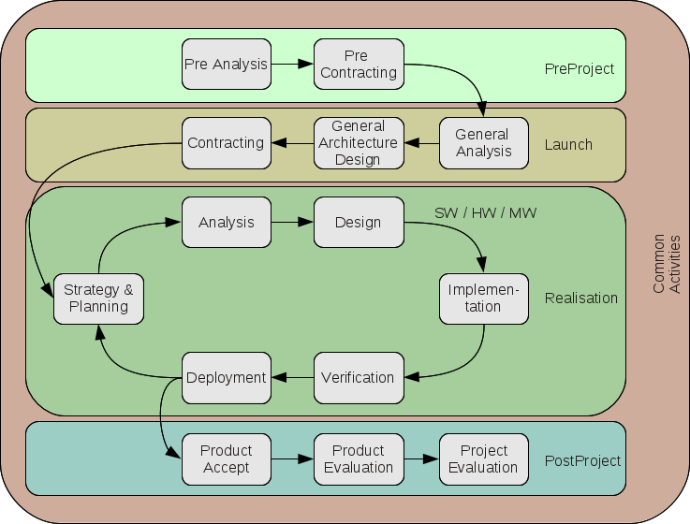
\includegraphics[width=0.5\textwidth]{./figurer/ij1.png}
  \caption{Udviklingsprocessen}
  \label{fig:ij1}
\end{figure}

\section{Kundens (undervisers) krav}
\label{sec:kravsspecifikation-1}
Nedenfor følger de krav, som er sat op af kunden, henholdsvis de krav som vi har specificeret for det færdige produkt.


\subsection{Funktionelle}
\label{sec:funktionelle}

\begin{itemize}
\item Udgangsspændingen fra HPP skal være kompatibel med spændingen på standardbatteripakken.
\item HPP skal startes enten elektrisk eller mekanisk med håndkraft.
\item Kapaciteten på HPP’en skal være tilstrækkelig til at lande dronen sikkert, hvis forbrændingsmotoren svigter.
\item HPP’en skal besidde en basal logning, så man kan udlæse performance.
\end{itemize}

\subsection{Designspecifikke }
\label{sec:designspecifikke-}

\begin{itemize}
\item Komponenter skal udvælges så de på bedste vis er et kompromis mellem lav vægt, pris og performance.
\item Brug så vidt muligt tilgængelige mekaniske dele - herunder forbrændingsmotor. 
\item En microcontroller skal sikre kontrol over systemet.
\end{itemize}

\section{Preprojekt}
\label{sec:preprojekt-}

For at synliggøre produktets formåen og berettigelse, har vi valgt at gengive vores storytelling og Rich Picture fra vore preprojekt. Begge har de til formål at give et meget generelt og råt overblik over systemet, på et niveau som alle kan forstå.

\subsection{Storytelling}
\label{sec:storytelling-}

Endelig er det lørdag! Du vågner alt for tidligt i bare spænding, for endelig er det lørdag, og du skal ud og flyve med drone. Dronecertifikatet er endelig i hus, og din store DJI S1000 drone er klar. Med batteriet på 100\%, smider du det hele i bilen og kører mod stranden. Der skal tages billeder af morgensolen fra helt nye vinkler. Med det påmonterede kamera, er det ingen sag.

Du ankommer til stranden, kaffen er drukket og du kan mærke hjerterytmen stige - nu skal det være. Du får, let og elegant, dronen i luften og taget nogle gode billeder. Pludselig, og uden varsel, vender dronen tilbage til dig. Du undrer dig meget, og først idet den lander foran dig, kommer du i tanke om den, mildest talt, elendige flyvetid dronen har på batteripakken. Kun omkring 15 minutter! Som du står der og ærgre dig, går de sidste skyer fra solen, og du kunne have fået de perfekte billeder du drømte om. 
Ovenstående scenarie har vi sat os for at undgå. Dette gøres ved at etablere en forbrændingsmotor og koble til dronens batterisystem gennem en generator. På denne måde lader dronen mens du flyver, og flyvetiden bliver forlænget markant!

\subsection{Rich Picture}
\label{sec:rich-picture-}

Herunder ses vores Rich Picture, som en konstrueret lige efter opgaven er blevet stillet.

\begin{figure}[h]
  \centering
  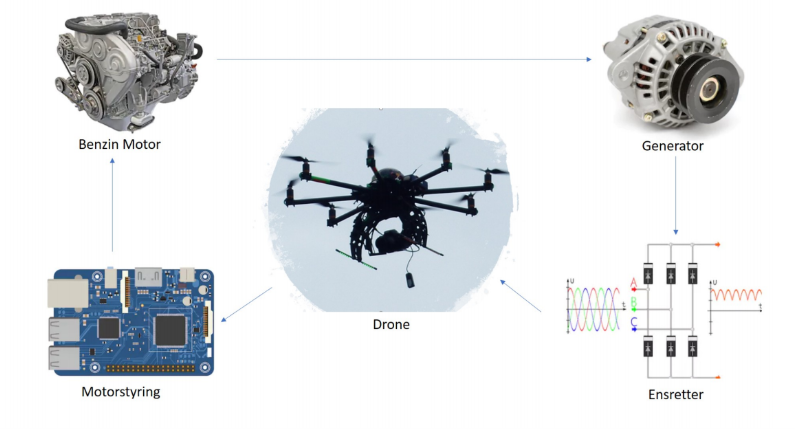
\includegraphics[width=0.5\textwidth]{./figurer/int1.png}
  \caption{Rich Picture}
  \label{fig:int1}
\end{figure}

\subsection{Kravspecifikation}
\label{sec:kravspecifikation}

På baggrund af ovenstående begyndte vi at opstille specifikke, tekniske krav til produktet - blandt andet på baggrund af de af underviserne stillede krav. I en kravsanalyse specificeres de krav, der er til det færdige produkt eller produktets enkelte komponenter. En udbytterig kravsanalyse indebærer at kunden inddrages. Kravene er nedenfor opstillet efter EARS-princippet (EARS:Easy to Approach Requirements Syntax).

Kravene er inddelt udfra ufravigelige (ubiquitous), begivenhedsorienterede (event-driven), driftsorienterede (state-driven) og fejlorienterede krav (unwanted behaviour). EARS-princippet muliggør således en prioritering af kravene.

\subsubsection{Ubiquitous}
\label{sec:kravspecifikation-1}

\begin{enumerate}[label=2.1.1.\arabic*]
\item Motoren skal kunne startes vha. BLDC-generator.
\item Udstødning skal monteres sådan at varmen ikke påvirker dronen.
\item Generatoren skal levere en middeleffekt på 2450 W ved 22,2 V (110,3 A)
\item Generatoren skal være 3-faset jf. projektbeskrivelsen.
\item HPP må maksimalt veje 5 kg.
\item Ensretteren skal kunne klare at håndtere en effekt af 2,45 kW.
\item Ensretteren skal modtage 3-faset vekselstrøm og levere en jævnstrøm.
\item HPP skal inddæmmes, så den kan modstå vejrforhold, jf. IP56 standard.
\item Ensretteren må maksimalt have ripple på 1V output.
\end{enumerate}

\subsubsection{Event Driven}
\label{sec:kravspecifikation-2}

\begin{enumerate}[label=2.1.2.\arabic*]
\item I tilfælde af nødlanding skal motoren deaktivere. 
\end{enumerate}

\subsubsection{State Driven}
\label{sec:kravspecifikation-3}

\begin{enumerate}[label=2.1.3.\arabic*]
\item HPP skal fungere korrekt før dronecopterens motorer igangsættes ved take-off.
\item Når motoren er aktiv, skal omdrejninger reguleres efter belastning af ladestrømmen.
\item Når generatoren ikke er i fulde omdrejninger, skal dronen ikke kunne lette.
\item Der skal defineres et effekt setpunkt til kontrol af opstart.
\item Når generatoren genererer strøm, skal input og output til/fra ensretteren overvåges og logges.
\end{enumerate}

\subsubsection{Unwanted}
\label{sec:kravspecifikation-4}

\begin{enumerate}[label=2.1.4.\arabic*]
\item Dronecopterens motorer vil tillade nødlanding ved fejl i moteren.
\item Hvis der opstår fejl i motoren, vil dronen lande når spændingen falder på batteriet.
\item Hvis generatoren ikke opnår fulde omdrejninger inden 10 sek. efter motorstart, afbrydes motoren.
\item Hvis udgangsstrømmen ikke når setpunktet (PID-regulering), skal dronen nødlande.
\end{enumerate}

\subsection{Blokdiagram}
\label{sec:blokdiagram-}

På baggrund af alt det ovenstående, samt flere andre overvejelser, som der kan læses mere om i den vedlagte preprojekt rapport, endte vi op med følgende blokdiagram over de forskellige subsystemer.

\begin{figure}[h]
  \centering
  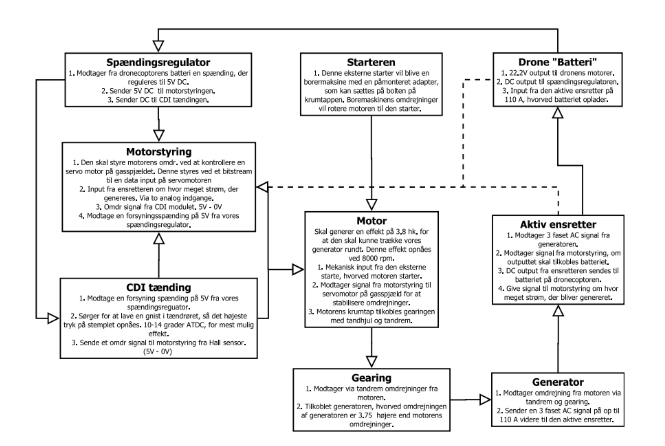
\includegraphics[width=0.5\textwidth]{./figurer/int2.png}
  \caption{Blokdiagram}
  \label{fig:int2}
\end{figure}
% \section{Hypotese}
% \label{sec:hypotese}

Da projektet er en videreførelse af et projekt fra tidligere BDE-studerende, der aldrig blev funktionelt, er der visse elementer der allerede foreligger. Forbrændingsmotoren, gearing og generatoren er allerede indkøbt. For at mindske omkostningerne ved projektet, har det været vores overbevisning, at vi ville bygge resten af projektet op om disse elementer. 

Da det ikke har været teknisk muligt at frakoble dronens allerede eksisterende batteri, har vi også været nødsaget til at bygge systemet op omkring dette. 

De vigtigste hovedelementer af systemet bliver således spændingsregulatoren, motorstyringen, og den aktive ensretter, hvilket også er de elementer der er beskrevet herunder.

\chapter{Baggrund}
\label{sec:baggrund}

\section{Aktive ensretter (Søren og Thomas)}
\label{sec:aktive-ensretter}

Ét af HPP’s primære subsystemer er blokken, der skal stå for ensretningen af den tre-fasede strøm/spænding, som genereres fra forbrændingsmotoren og generatoren. Der har været arbejdet med  mange essentielle dilemmaer og prioriteter, der skulle afklares for at få den mest optimale løsning. Da der foreligger et grundlæggende ønske om at holde den samlede vægt på HPP nede på et acceptabelt niveau, var det nærliggende at forsøge at realisere ensretningen aktivt. Hvad dette vil sige, berøres i det efterfølgende afsnit.

\subsection{Passiv vs. aktiv ensretning}
\label{sec:passiv-vs.-aktiv}

I en typisk ensretter (en passiv ensretter) anvendes en diodekonstruktion, som tillader et AC-signals positive cyklus at passere til outputtet, for derefter at invertere den negative del af cyklussen. Resultatet er et udelukkende positivt signal, med en variabel spændingsamplitude. Da vi forventer at lede ca. op til max. 100 A\footnote{Se bilag, Timebox 1 og 2, for yderligere information.} (peak) gennem systemet, er dioder ikke anvendelige. Spændingsfaldet over dioder ligger typisk i omegnen af 0.3-0.7 V, og det vil betyde et effektab, som motoren skal kompensere for via flere omdrejninger.

I stedet kan der anvendes IDC (\textit{Ideal Diode Controller}), som har til formål at levere spænding til gate-terminalen på MOSFET transistorer. En MOSFET har i \textit{cut-off} tilstand en diodelignende opførsel, men når de leder optimalt, er modstanden i transistoren meget lav (helt ned til få m$\Omega$). Parallelkobles transistorerne kan modstand sænkes yderligere. IDC’en styrer, hvornår transistorerne åbner og lukker, og kontrollerer dermed AC-signalets passage gennem ensretteren, så output-signalet er positivt, ligesom ved en almindelig diode-ensretter. Denne styring gør, at ensretteren defineres som en aktiv ensretter.
\clearpage
\begin{figure}[h]
  \centering
  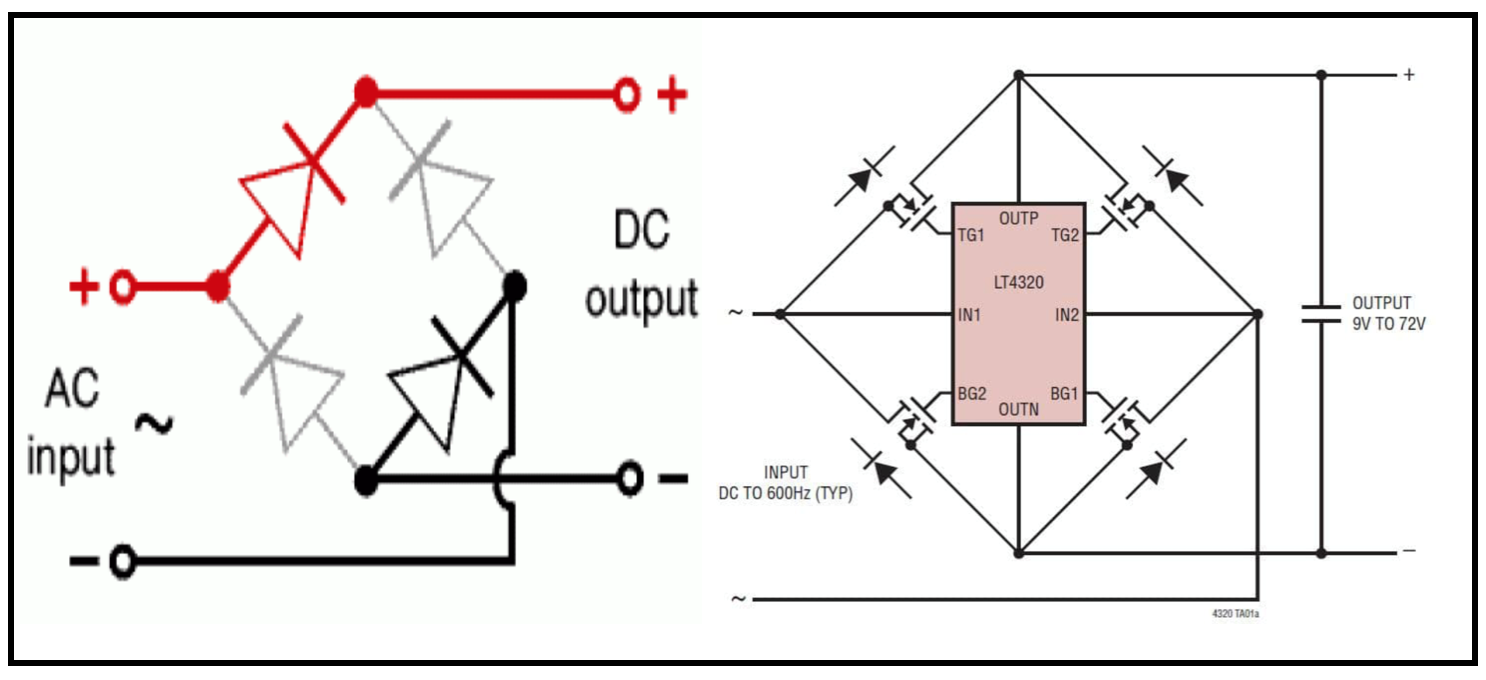
\includegraphics[width=0.6\textwidth]{./figurer/prens1.png}
  \caption{Passiv vs. aktiv ensretning}
  \label{fig:prens1}
\end{figure}

Den store fordel ved aktiv ensretning kontra passiv er reduceringen af effekttabet gennem kredsløbet. Denne reduktion påvirker direkte, at forbrændingsmotoren skal køre med mindre RPM for at producere behovet til dronen, end hvis ensretningen var passiv. Derudover vil dimensioneringen af heatzinks til kredsløbet ligeledes være væsentlig mindre, da mindre effekttab betyder mindre varmeafledning.  
  
En generel udfordring ved AC/DC konvertering er \textit{ripples} på output signalet. Ensrettes en enkelt AC-fase, får man et udgangssignal, med stor variation i spænding leveret. Kombineres tre faser med en faseforskydning på 120$^\circ$ mellem sig. I vores tilfælde, vil summationen af de tre sinuskurver generere et output signal med mindre \textit{ripple}.

\begin{figure}[h]
  \centering
  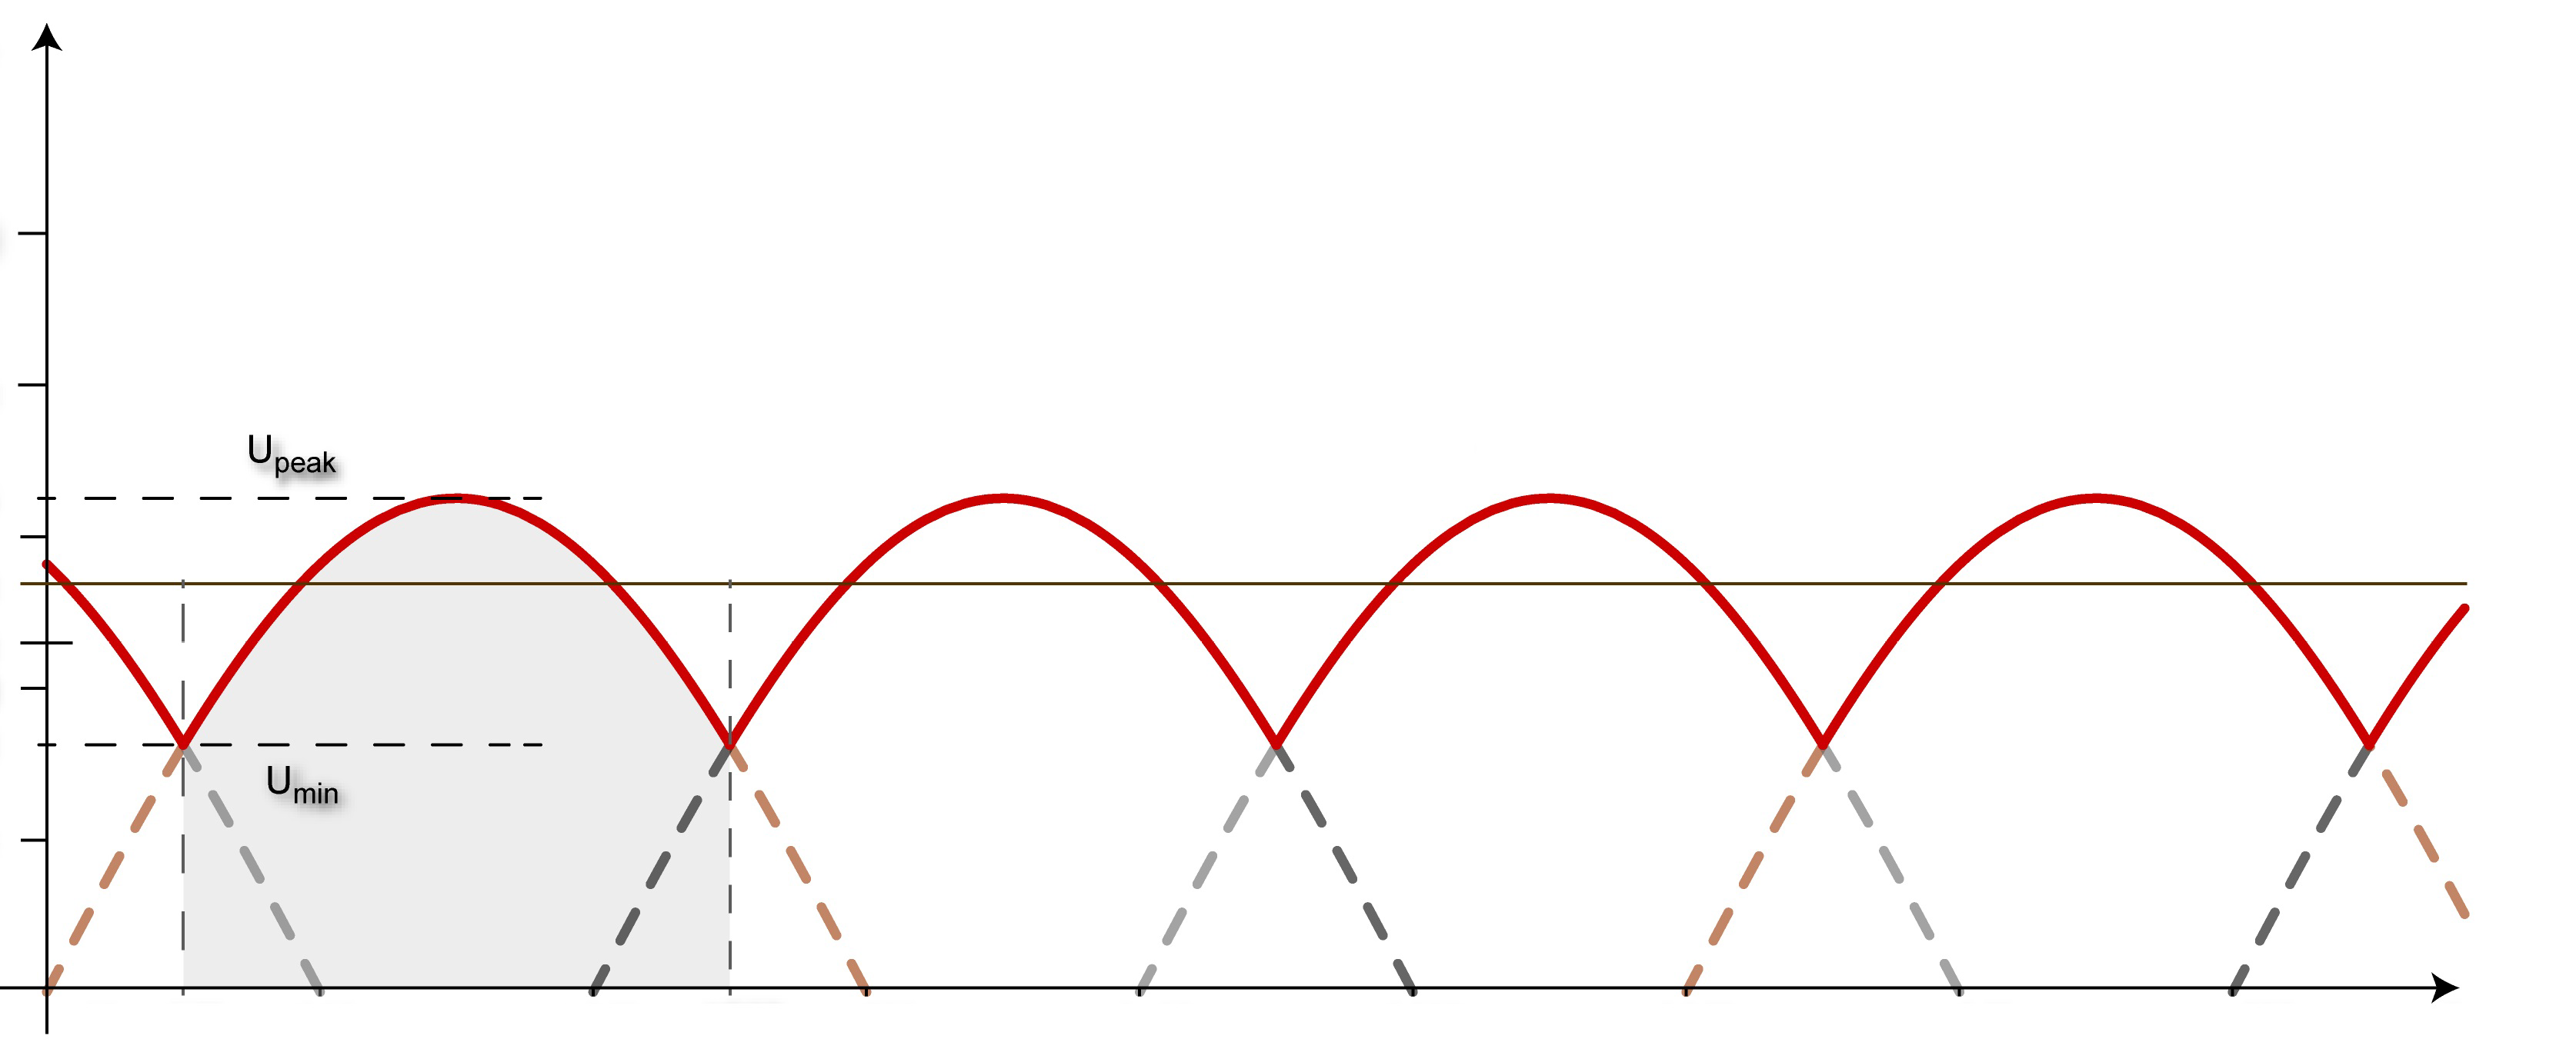
\includegraphics[width=0.5\textwidth]{./figurer/prens2.png}
  \caption{Graf over ripple spænding på output signal som funktion af tid. Stiplet linje = ensrettet enkeltfase
AC-signal. Rød linje = ripple på kredsløb med kondensator parallelt på load. Kilde: Wikimedia Commons}
  \label{fig:prens2}
\end{figure}

Der vil stadig være \textit{ripple} til stede i signalet, og denne udjævnes til et acceptabelt niveau (for batteriet på dronen) vha. kondensatorer. Kondensatoren lader, når $\frac{\mathrm{d}v}{\mathrm{d}t}$ på udgangssignalet er positivt og aflader, når spændingen igen falder. Den strøm kondensatoren afgiver adderes til udgangssignalet, hvorfor $\frac{\mathrm{d}v}{\mathrm{d}t}$ øges.

\subsection{Valg af IC }
\label{sec:valg-af-ic}

I timebox 2 analyserede vi os frem til følgende valg af IDC til realiseringen af kredsløbet til den aktive ensretter:
\begin{itemize}
\item Linear Technology, LT4320-1, Ideal Diode Bridge Controller
\end{itemize}

Dette skyldes bl.a., at den er designet specifikt til luftbårne strømforsyningssystemer, som kan håndtere frekvenser op til 600 Hz, 9-72V, og opfylder tidligere defineret krav om optimal effektivitet, og minimalt effekttab.

\afterpage{
\begin{figure}[h]
  % \begin{minipage}{\textwidth}
    \centering
    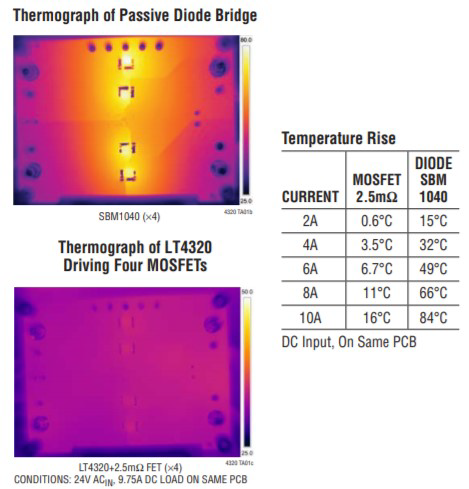
\includegraphics[width=0.3\textwidth]{./figurer/prens3.png}
    \caption[Varmeudvikling. Passiv vs. LT4320]{Varmeudvikling. Passiv vs. LT4320\protect\footnotemark}
    \label{fig:prens3}
  % \end{minipage}
\end{figure}
\footnotetext{Fra databladet til LT4320-1. \url{https://www.analog.com/media/en/technical-documentation/data-sheets/4320fb.pdf}}
}
\clearpage
\subsection{Kredsløbet}
\label{sec:kredslobet}

Leverandøren af LT-4320-1, foreslår kredsløbet\footnote{\url{https://www.analog.com/en/products/lt4320.html}} set på figur \ref{fig:prens2}, som en yderst energieffektiv tre-faset aktiv ensretter.

\begin{figure}[h]
  \centering
  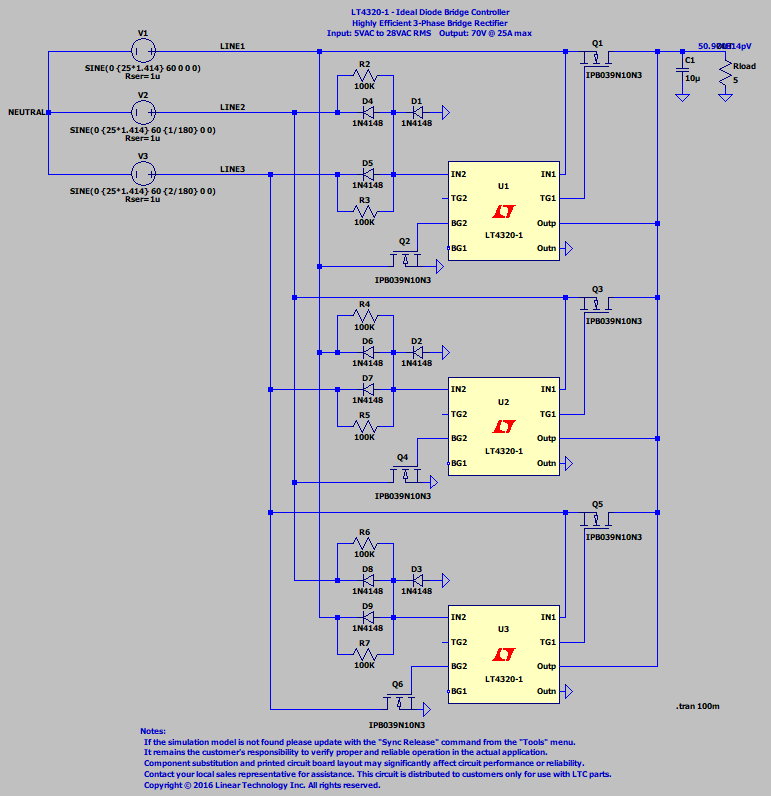
\includegraphics[width=0.5\textwidth]{./figurer/prens4.png}
  \caption{Kredsløb til realiseringen af ensretteren}
  \label{fig:prens2}
\end{figure}

Vi valgte at arbejde videre med den opstilling. De næste afsnit indeholder en opsummering af simulering, realiseringen og test af kredsløbet.

\section{Spændingsregulator (Jacob)}
\label{sec:spandingsforstarker}

Som en del af det samlede produkt har vi behov for en spændingsregulator. Dette skyldes, at batteriet har en spændings på 22 V, som skal konvereteres til 5 V for at kunne forsyne microcontroller, servomotor samt tændspole. %, hvilket også er udgangsspændingen fra generatoren. Men da vores motorstyring skal forsynes med 5 V DC, skal vi have spændingen reguleret ned. 
% Den kommende del omfatter kravspecifikation, analyse, design, implementering og verifikation af vores spændingsregulator. 

\subsection{Kravsspecifikation}
\label{sec:kravsspecifikation-2}

\subsubsection{Uniquitous Requirements}
\label{sec:kravsspecifikation-3}

\begin{itemize}
\item Spændingsregulatoren skal kunne regulere en spænding fra 22 V ned til 5 V, med en pålydende strøm af 1 A. 
\item Spændingsregulatoren skal være vejrbestandig.
\end{itemize}

Efter research af forskellige muligheder for spændingsregulering, kom vi frem til tre reelle muligheder. Én baserer sig på LM78xx-serien, én baseret på LM317 og én baseret på en BUCK-converter.

\subsection{Generel analyse}
\label{sec:generel-analyse-}

Den generelle analyse omhandler udelukkende den sammenhæng, som spændingsregulatoren skal sidde i.

\subsubsection{Interface Analysis and Design}
\label{sec:generel-analyse}

Spændingsregulatoren vil være koblet til batteripakken i den ene ende og de logiske kredsløb i den anden ende. Som både indgang og udgang til spændingsregulatoren, vil der være forbundet almindelige ledere - 1 kvadrat som indgang og 0,5 kvadrat som udgang.

\begin{figure}[h]
  \centering
  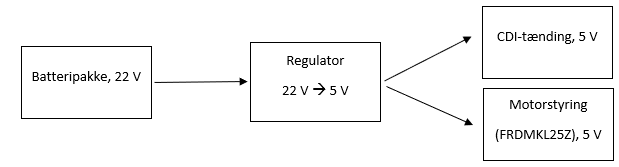
\includegraphics[width=0.5\textwidth]{./figurer/j1.png}
  \caption{Interface analysis}
  \label{fig:j1}
\end{figure}

Figur \ref{fig:j1} viser interface analysis.

\subsubsection{Dimensionering}
\label{sec:generel-analyse-1}

Da spændingsregulatoren er en blivende del af systemet, er vi afhængige af, at holdbarheden er god, og som minimum lever op til kvaliteten af de resterende dele af produktet.

Ét af de problemer vi kan støde på under spændingsregulering af temperaturforøgelse, der kan brænde komponenten af.

\subsubsection{Structural Analysis}
\label{sec:generel-analyse-2}

Spændingsregulatoren skal være vejrbestandig, da dronen skal kunne være udendørs i alle slags vejr. For at spændingsregulatoren kan blive det, skal den pakkes ind i en boks, der sikres efter IP66 standard. Problemet med dette er, at regulatoren udvikler en hel del varme. Derfor skal spændingsregulatoren være i en kasse for sig, hvor heatsink monteres udvendigt på kassen.

\section{Motorstyring (Simon)}
\label{sec:motorstyring}

Motorstyringen for systemet vil bestå i præcis justering af forbrændingsmotorens omdrejninger i forhold til dronecopterens strømforbrug. Det valgtes at arbejde med et simplere system for at fokuserer på principperne i motorstyring. Det betød at motorstyringen skulle bestå i udvikling af PID-regulering af forbrændingsmotoren sådan at der skulle foregå korrektion af motorens spjældvinkel i forhold til motorens omdrejninger.

% Målet med dette afsnit er at opstille en kravsspecifikation for motorstyringen samt at færdiggøre analysen af motorstyringen og lægge op til hvordan en test af motorstyring kan udformes for at præcisere PID-algoritme samt at opfylde krav.

% \lstdefinestyle{customc}{
%   belowcaptionskip=1\baselineskip,
%   breaklines=true,
%   frame=L,
%   xleftmargin=\parindent,
%   language=C,
%   showstringspaces=false,
%   basicstyle=\footnotesize\ttfamily,
%   keywordstyle=\bfseries\color{green!40!black},
%   commentstyle=\itshape\color{purple!40!black},
%   identifierstyle=\color{blue},
%   stringstyle=\color{orange},
% }

% \lstdefinestyle{customasm}{
%   belowcaptionskip=1\baselineskip,
%   frame=L,
%   xleftmargin=\parindent,
%   language=[x86masm]Assembler,
%   basicstyle=\footnotesize\ttfamily,
%   commentstyle=\itshape\color{purple!40!black},
% }

% \lstset{escapechar=@,style=customc}

\subsection{Kravsspecifikation}
\label{sec:kravsspecifikation}
For at fremstille en kravsspecifikation til motorstyring søges i litteraturen efter beskrivelsen af løsning på lignende problemstilling. Fjare\autocite{pid1} er en artikel, der beskriver PID-regulering af en forbrændingsmotor som skal drive en aerocopter. Med baggrund i Fjare\autocite{pid1} sættes følgende krav, som forsættelse svarende til afsnit 2.1.3 (State-Driven requirements) i launch-fase rapporten (se bilag):
\begin{enumerate}[label=2.1.3.\arabic*]
\item Overshoot skal ikke være mere en 197 rpm.
\item Justeringstiden må max være 8,8 sekunder.
\item Ifm. et step respons skal 90 \% af steady-state være opnået i mindre end 3 sekunder.
\item Strømforsyningen til dronecopterens propelmoterer skal justeres sådan at dronecopterens hastighed kan holdes konstant.%Det skal være muligt at vedligeholde en konstant hastighed over længere tid (dvs. mere end 5 minutter).
\item Servomotoren skal kunne reguleres.
\item Motoren skal kunne startes.
\item Omdrejningerne skal kunne måles.
\end{enumerate}

\subsection{Motorstart}
\label{sec:esc}

En ``electronic speed control'' (ESC) anvendes som fartstyring i fartøjer. En ESC tager et input signal, fx fra en pedal eller et joystick, og genererer et signal udfra et netværk af transistorer (FETs). Signalet kan varieres ved at varierer transistorernes switching.

Alt efter om en motor er brushed eller brushless kræves forskellige ESC'er. I projektets tilfælde er der tale om en brushless motor. 

ESC'er kan i nogen tilfælde programmeres. Ved programmering kan følgende typisk redigeres:
\begin{itemize}
\item Timing
\item Acceleration
\item Deccelaration
\item Rotationsretning
\end{itemize}

ESC'en skal genererer et trefaset signal. Fasen varierer med motor rotation og en Hall sensor bruges til at registrerer omdrejningerne. Brugerens interaktion med starteren er basal og jf. launch fase rapport, er brugerinteraktion med hele HPP minimal.

Når der vælges en ESC er der flere ting at tage højde for. For det første brushed vs. brushless motor. Herefter er der spændings- og strømstyrke begrænsninger for ESC for hvor meget den kan håndtere. Spændingsbegrænsningen er oftest udtrykt i antal battericeller. NiMH batterier har 1,2 V pr. celle og Lithium batterier har 3,7 V pr. celle. En markering i datablad kan indeholde grænser for begge batterityper. ESC'en vil skulle kunne håndterer 22 V da dronens batteri leverer denne spænding. Det planlægges at anvende  en ``Turnigy Plush 60a'' (TP60a). TP60a er ratet til 2-6 Li-ion batterier (optil 22,2 V) eller 5-18 (optil 21,6 V) NiMH batterier. Altså en grænse omkring 22 V. Grænsen for kontinuerlig strømstyrke ligger på 60 A.

Dronebatteriet, et Lithium Poly batteri med 6 celler, vil ved opkobling til ESC'en kunne generere et trefaset signal som sendes til generatoren.

\subsection{Regulering af hastighed}
\label{sec:regul-af-hast}

Ved regulering af forbrændingsmotorens hastigheder reguleres motorens gasspjæld. Der anvendes en servomotor påsat gasspjældet.

For at kunne udvælge en passende servomotor til system-to-be, opstilles herunder følgende krav:
\vspace{1em}
\begin{tabular}[h]{ll}
2.1.1.13&Servomotoren skal have en forsyningsspænding på 5 volt.\vspace{0.5em}\\
2.1.1.14&Servomotoren skal veje under 15 g.\vspace{0.5em}\\
2.1.3.6 &Reaktionshastighed på minimum 0,15 s/60$^\circ$.\vspace{0.5em}\\
2.1.3.7& Servomotorens skal have et moment (torque) på minimum 1,5 kg/cm.\vspace{0.5em}\\
2.1.3.8& Servomotoren skal kunne styres via et PWM signal.\vspace{0.5em}\\ 
\end{tabular}
\vspace{1em}\\
\noindent \textbf{Ad 2.1.1.13}

\noindent Siden der skal anvendes en spændingsregulator, der konverterer dronecoptorens batterispænding fra 22,2 volt ned til 5 volt, ville det være fordelagtigt at vælge en servomotor, der skal forsynes med 5 volt.

Der anvendes en servomotor, TowerPro SG-90, som ses i \ref{fig:anath2}

\begin{figure}[h]
  \centering
  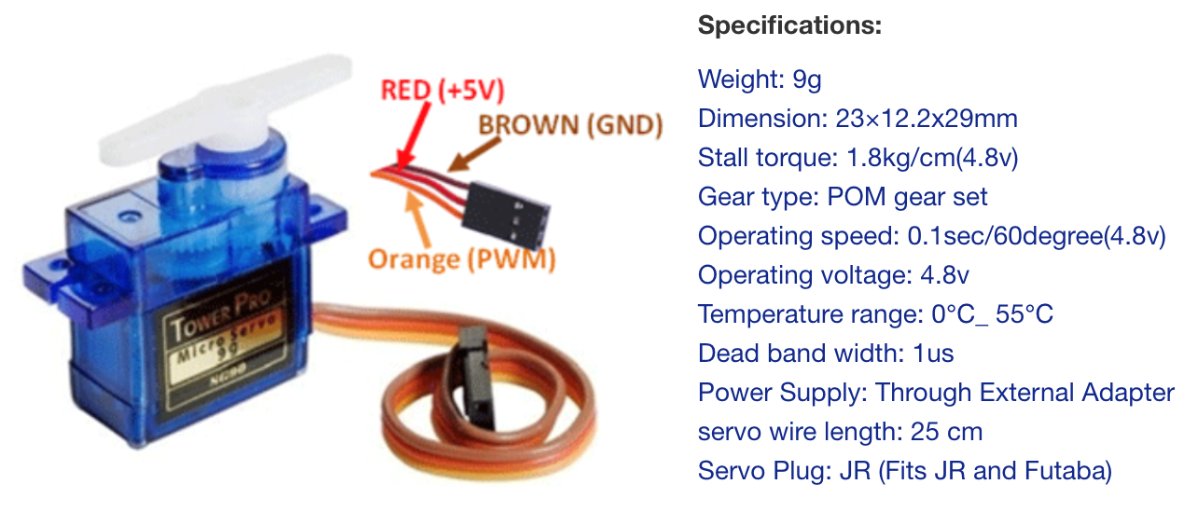
\includegraphics[width=0.7\textwidth]{anath2.png}
  \caption{TowerPro SG-90. Kilde: \url{http://www.towerpro.com.tw/product/sg90-7/}}
  \label{fig:anath2}
\end{figure}

Som des ses ud fra servoens specifikationer lever denne op til de opstillede krav. Derudover er dimensionerne på servoen meget små, hvilket er at foretrække til HPP.

I figur~\ref{fig:anath3} ses opsætningen af duty-cycle for servomotoren. Signalet skal have en frekvens på 50 Hz, og on-time for en periode skal være mellem 1 og 2 ms. Det vil sige, at servoens styrearm står med en vinkel på $0^\circ$, når on-time er 1,0 ms, $90^\circ$ med en on-time på 1,5 ms, og $180^\circ$ med on-time på 2,0 ms. 

\begin{figure}[h]
  \centering
  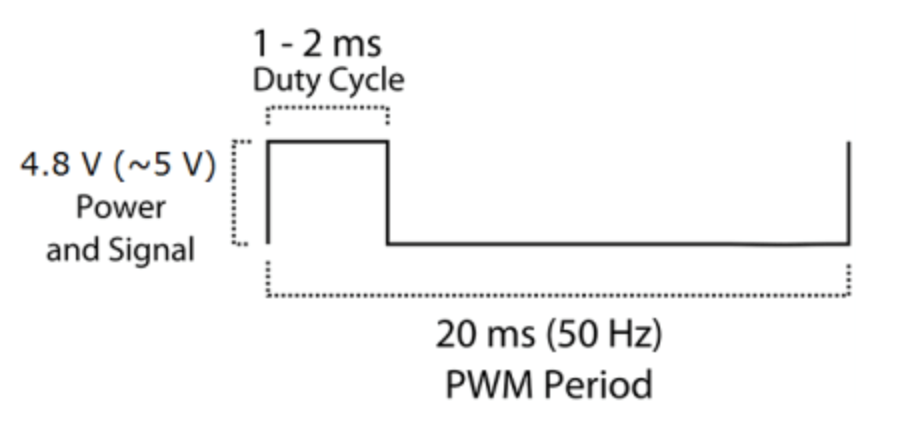
\includegraphics[width=0.5\textwidth]{anath3.png}
  \caption{PWM signal til servomotoren}
  \label{fig:anath3}
\end{figure}

\subsection{PID regulering}
\label{sec:overordnet-mal}

PID-regulering består i regulering af et output på baggrund af forskellen mellem det tilstræbte og det faktiske - dette kan kaldes fejlen. PID regulering kan beskrives med
\begin{equation}
  \label{eq:1}
  u(t)=k_Pe(t)+k_I \int_0^t e(\tau)\mathrm{d}\tau + k_D\frac{\mathrm{d}e(t)}{\mathrm{d}t}
\end{equation}

hvor $e(t)$ er fejl som funktion af tiden, $e(\tau)$ er fejl som funktion af den akkumulerede tid og $k_P$, $k_I$ og $k_D$ er koefficienter svarende til henholdsvis det proportionale, integrede og deriverede forhold. Det proportionale vil sige forholdet mellem tilstræbte og det faktiske for et givent tidspunkt. Det integrede vil sige forskellen mellem det tilstræbte og det faktisk akkummulerede over tid. Det betyder at den integrerede koefficient viser en trend for fejlen. Det deriverede er et mål for hvor hurtigt fejlen ændrer sig over tid.

Formålet ved udarbejdelse af PID-regulering er at finde de optimale værdier af $k_P$, $k_i$ og $k_d$.

% For et givent sæt af K-værdier, udvælges en række forskellige typer af trinvise ændringer i hastigheden. Der måles på hvor lang tid det tager for ændringen at indfinde sig, samt hvor store udsving dette gør sig ud i.

Som udgangspunkt er det tidligere vist(\autocite{pid1}) at $K_p=0,065$ og $K_i=0,000005$ har været optimale, samt at $K_d$ helt blev droppet eftersom det ikke var en gavnlig parameter.

\subsection{Software}
\label{sec:software}

Fra Fjare\autocite{pid1} kunne et eksempel på et program være skrevet i pseudo C-kode:
\begin{lstlisting}[language=C,basicstyle=\ttfamily]
  void velPID ( ) {
    lowpassSpeed = alpha * lastLowpassSpeed + (1-alpha) * measuredSpeed;
    K1 = kp * setpointWeight * (setpointSpeed - lastSetpointSpeed) + kp * (lastMeasuredSpeed - lowpassSpeed);
    K2 = ki * (setpointSpeed - lowpassSpeed);
    K3 = kd * (2 * lastMeasuredSpeed - lowpassSpeed - lastLastMeasuredSpeed);
    output = lastOutput - K1 - K2 - K3;
    throttlePos = floor(output + 0.5);
    if(throttlePos<throttleopen){
      output = (double) throttleopen;
      throttlePos=throttleopen;
    }
    if(throttlePos>throttlesafe){
      output = ( double )throttlesafe;
      throttlePos=throttlesafe;
    }
    lastLowpassSpeed = lowpassSpeed;
    lastLastMeasuredSpeed = lastMeasuredSpeed;
    lastMeasuredSpeed = lowpassSpeed;
    lastSetpointSpeed = setpointSpeed;
    lastOutput = output;
    throttle.writeMicroseconds(throttlePos);
  }
\end{lstlisting}

I koden anvendes et lavpasfilter (\lstinline{lowpassSpeed}) for at mindske ændringen (beregningen af \lstinline{K1}, \lstinline{K2} og \lstinline{K3}) for hver regulering. \lstinline{alpha} sætter størrelsen af filteres (0 er ingen filter). \lstinline{setpointSpeed} sættes til den ønskede hastighed. Koden kontrollerer output ved på baggrund af sidste output at fra trække \lstinline{K1}, \lstinline{K2} og \lstinline{K3}.


\chapter[Metoder]{Metoder og analyser}
\label{sec:metode}

\section{Aktive ensretter (Søren og Thomas)}
\label{sec:aktive-ensr-soren}

\subsection{Test af generators output spænding}
\label{sec:test-af-generators}

Inden vi anskaffede os IC’erne til kredsløbet, skulle det sikres, at forbrændingsmotor og generator i tomgangsdrift, som minimum producerede 9 V (peak). Dette var nødvendigt for, at IC’erne var funktionsdygtige. \textcolor{black}{Der opstilles som følge af ovenstående konstatering et krav til den aktive ensretter.}

\begin{tabular}{p{1cm}l}
  \textcolor{black}{2.1.3.9}&\textcolor{black}{Der skal som minimum være 9 Volt (peak) på udgangen af generatoren,}\\
  & \textcolor{black}{inden denne tilkobles den aktive ensretter}
\end{tabular}

For at verificere dette blev der konstrueret et testsetup, hvor det var muligt at måle output spændingen på én af generatorens tre faser. Et blokdiagram over testsetuppet kan ses i figur \ref{fig:prens5}.

\begin{figure}[h]
  \centering
  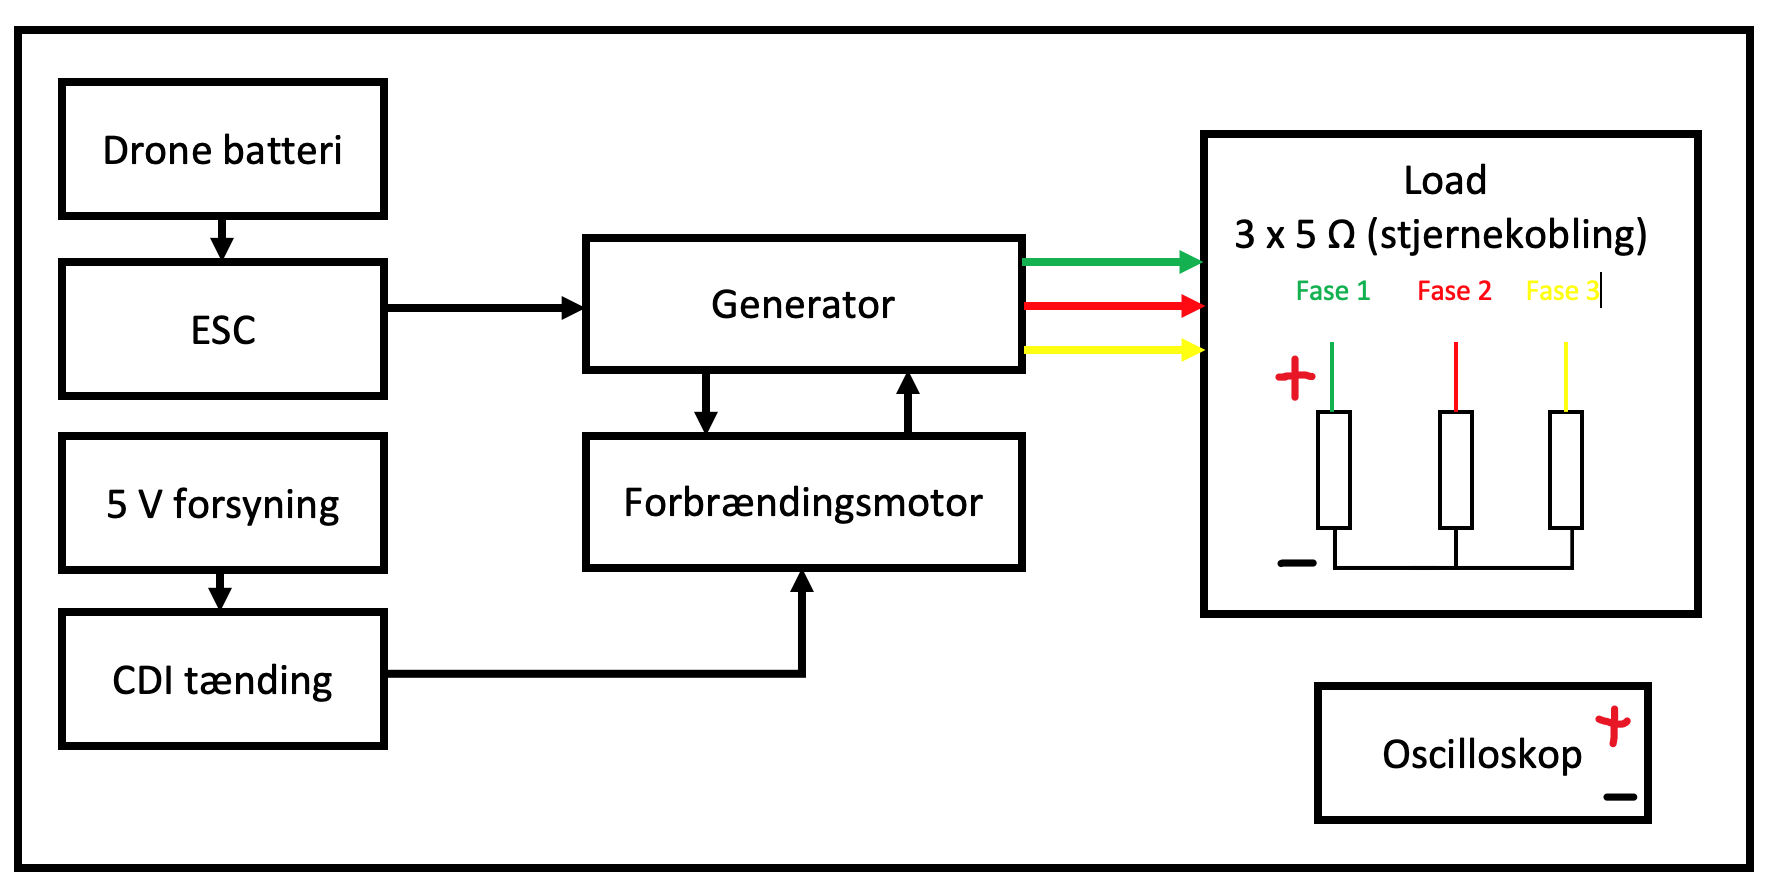
\includegraphics[width=0.5\textwidth]{./figurer/prens5.png}
  \caption{Blokdiagram til test af outout spænding på en fase af generator}
  \label{fig:prens5}
\end{figure}

Testen viste, at der var en spænding på 11.4 V (peak)\footnote{Se bilag, Timebox 6, for yderligere information.} på én af generatorens faser med forbrændingsmotoren kørende i tomgang. Ud fra resultatet af denne test var det bekræftet, at der altid ville være et tilstrækkeligt spændingsniveau som input til ensretteren. Derfor indkøbte vi IC’erne med henblik på videre konstruktion af kredsløb.

\subsection{Simulering}
\label{sec:simulering}

Inden vi påbegyndte opbygningen af den aktive ensretter, blev funktionaliteten simuleret vha. programmet, LT-spice, som er leveret af IC’ens producent, \textit{Linear Technology}.

Figur\ref{fig:prens6} viser et skærmbillede af simuleringen. Det fremgår tydeligt, at outputtet (\textit{lyseblå}) er ensrettet i forhold til faserne (\textit{grøn, rød og blå}) til et tilnærmelsesvist DC niveau. 

\begin{figure}[h]
  \centering
  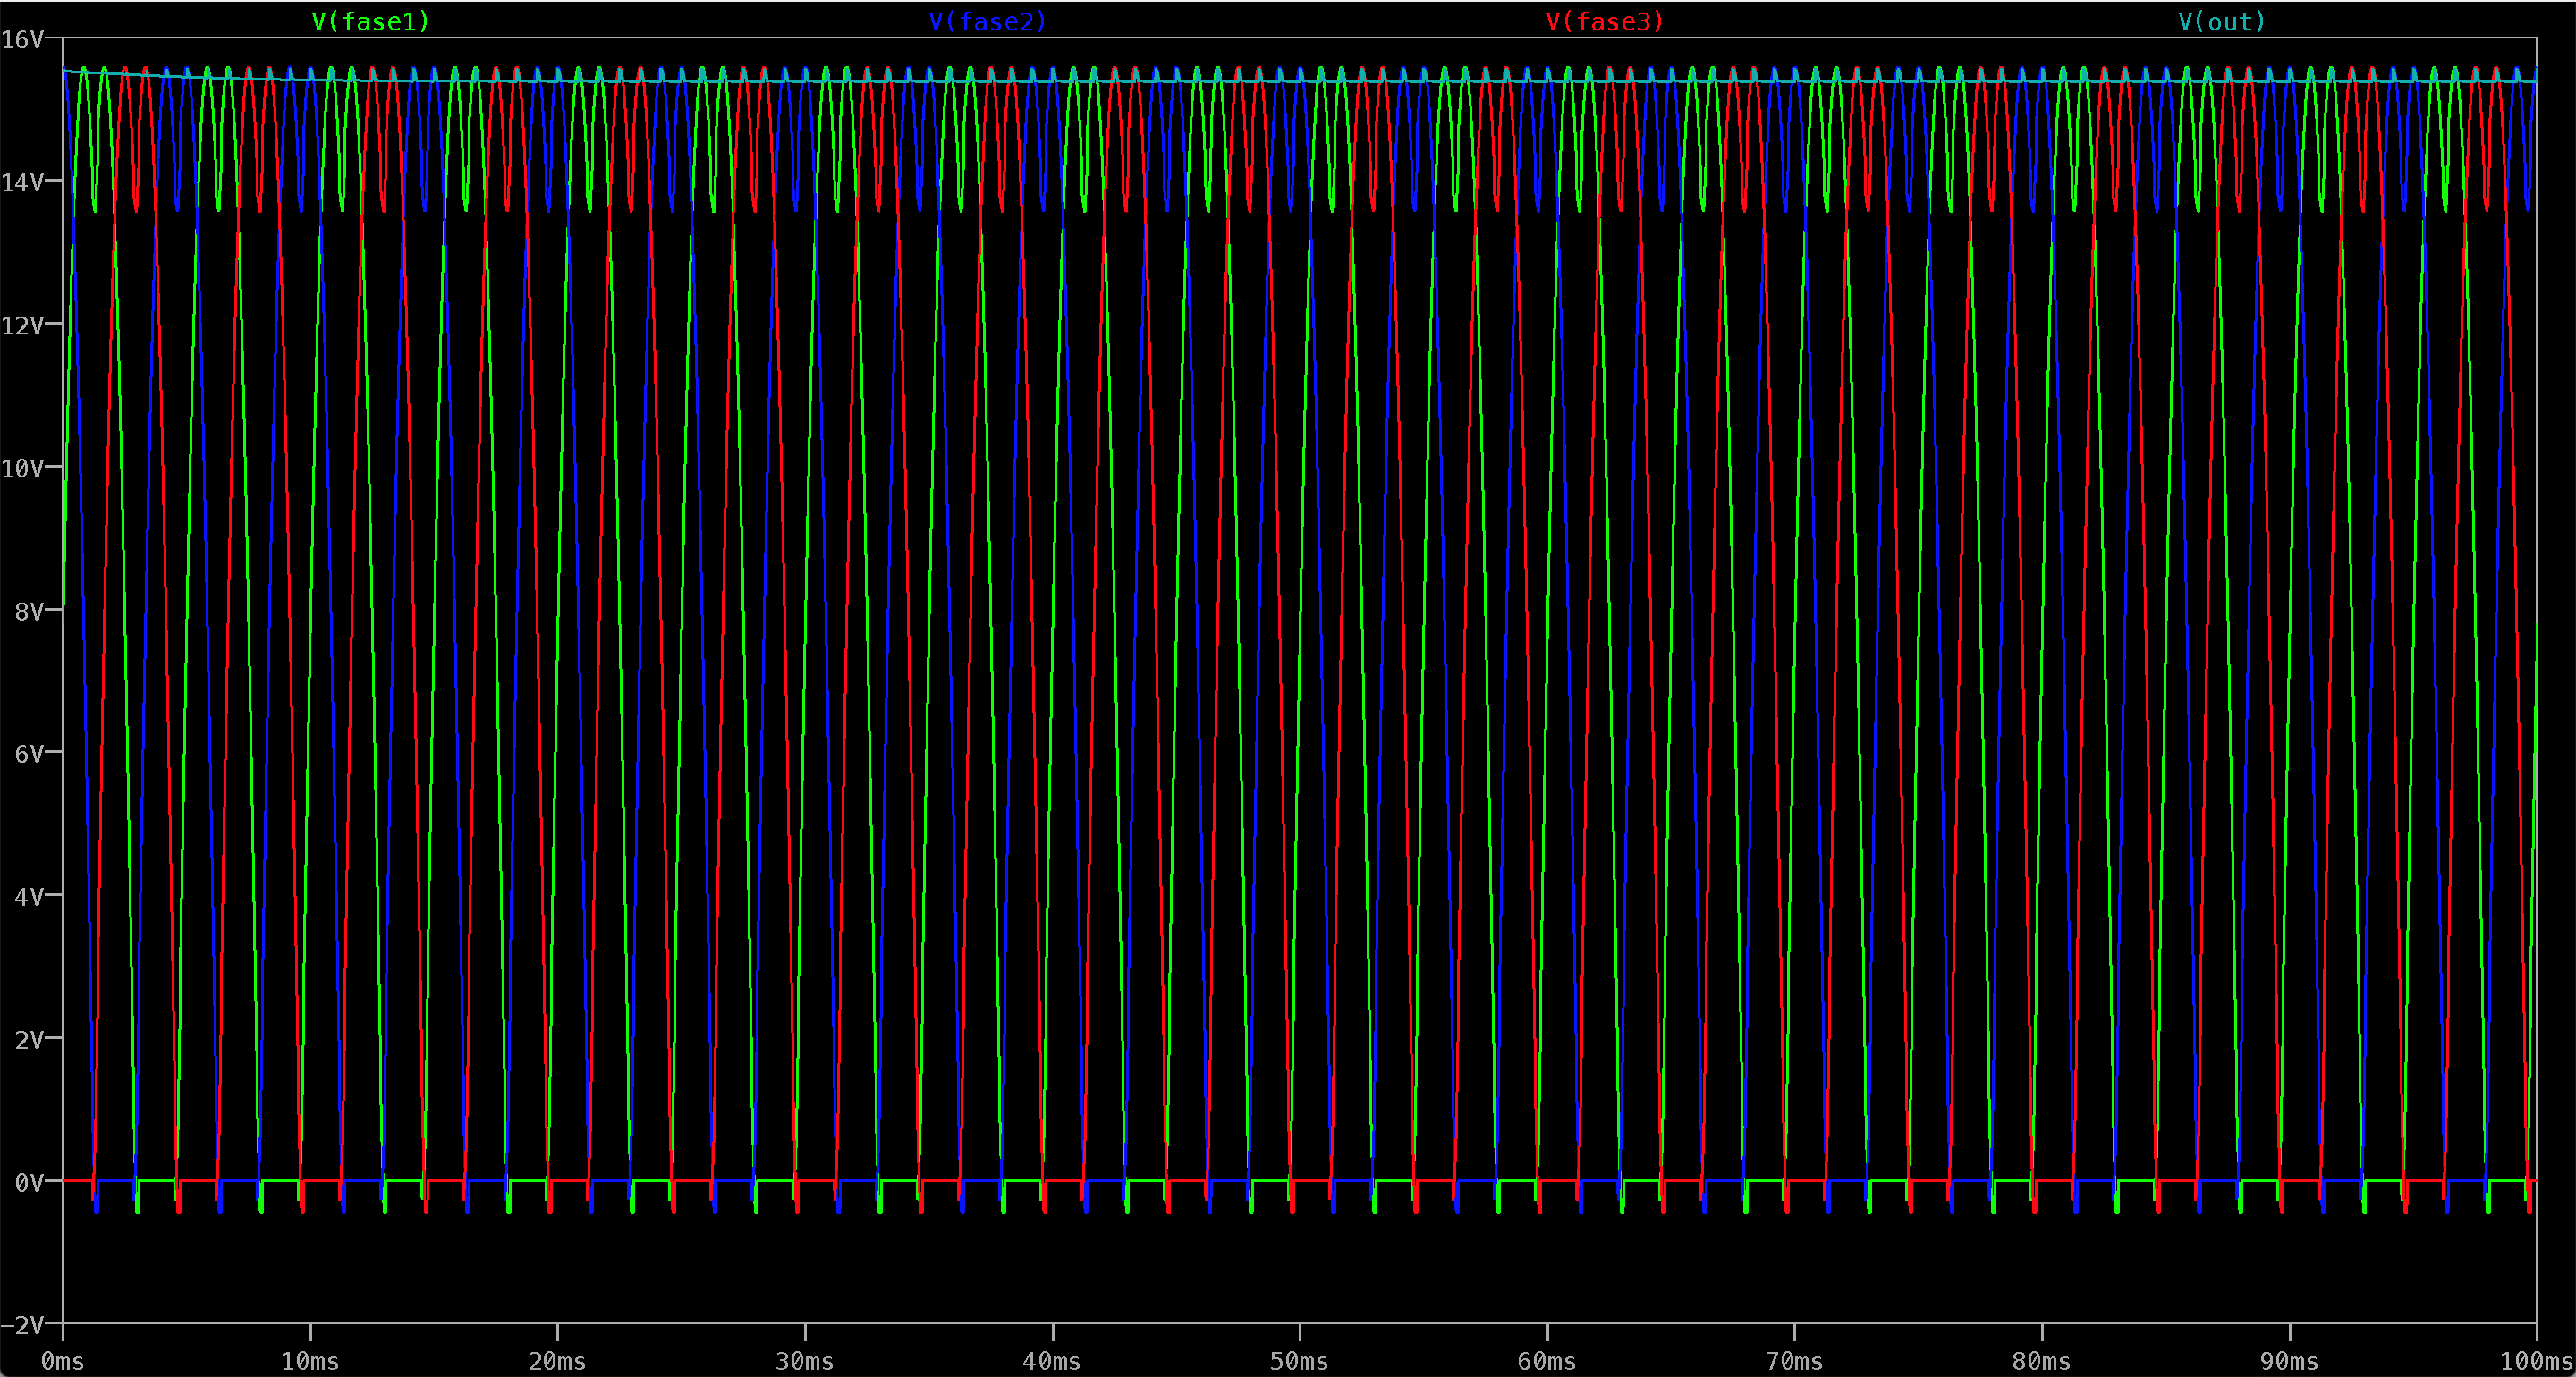
\includegraphics[width=0.9\textwidth]{./figurer/prens6.png}
  \caption{Resultat af simuleringen. \textcolor{cyan}{$V_{out}$: Målingen over load modstanden}, \textcolor{green}{$V_{fase1}$: Målingen af fase 1}, \textcolor{blue}{$V_{fase2}$: Målingen af fase 2}, \textcolor{red}{$V_{fase1}$: Målingen af fase 1}}
  \label{fig:prens6}
\end{figure}

Det skal nævnes, at skaleringen af komponenter i det simulerede kredsløb ikke er identisk med det tiltænkte. Simuleringen er udført for at konstatere kredsløbets teoretiske funktionalitet.

Ud fra resultatet\footnote{Se bilag, Timebox 7, for yderligere information.} i simuleringen var vi overbevist om, at kredsløbet i teorien kunne leve op til den ønskede funktionalitet. Næste del af processen var derfor at opbygge kredsløbet på et breadboard i en nedskaleret version.

\subsection{Teststand}
\label{sec:teststand}

Da der var behov for at have et setup, hvor der problemløst kunne genereres en trefaset spænding til at teste den aktive ensretter, besluttede vi, at det ikke var sikkerhedsmæssigt forsvarligt indtil videre at benytte forbrændingsmotoren til at drive generatoren. Vi har fra start af været i besiddelse af en ekstra BLDC motor, og hvis denne forbindes med den oprindelige generator, vil det derved være muligt at generere en trefaset spænding.

Den oprindelig stand med påmonteret forbrændingsmotor og generator benyttes til den nye teststand. Tandremmen mellem forbrændingsmotor og generatoren afmonteres, hvorefter standen boltes fast til en træ reglar med dimensionerne, 5x10x45 cm. Den ekstra BLDC motor boltes fast til en jernplade med to stålklemmer, hvorefter jernpladen påmonteres træ reglaren i passende afstand til den oprindelige BLDC motor. Herefter forbindes akslen på de to motorer med en ny tandrem. I figur \ref{fig:nt1} og \ref{fig:nt2} ses billeder af den færdige teststand.
\clearpage
\begin{figure}[h]
  \centering
  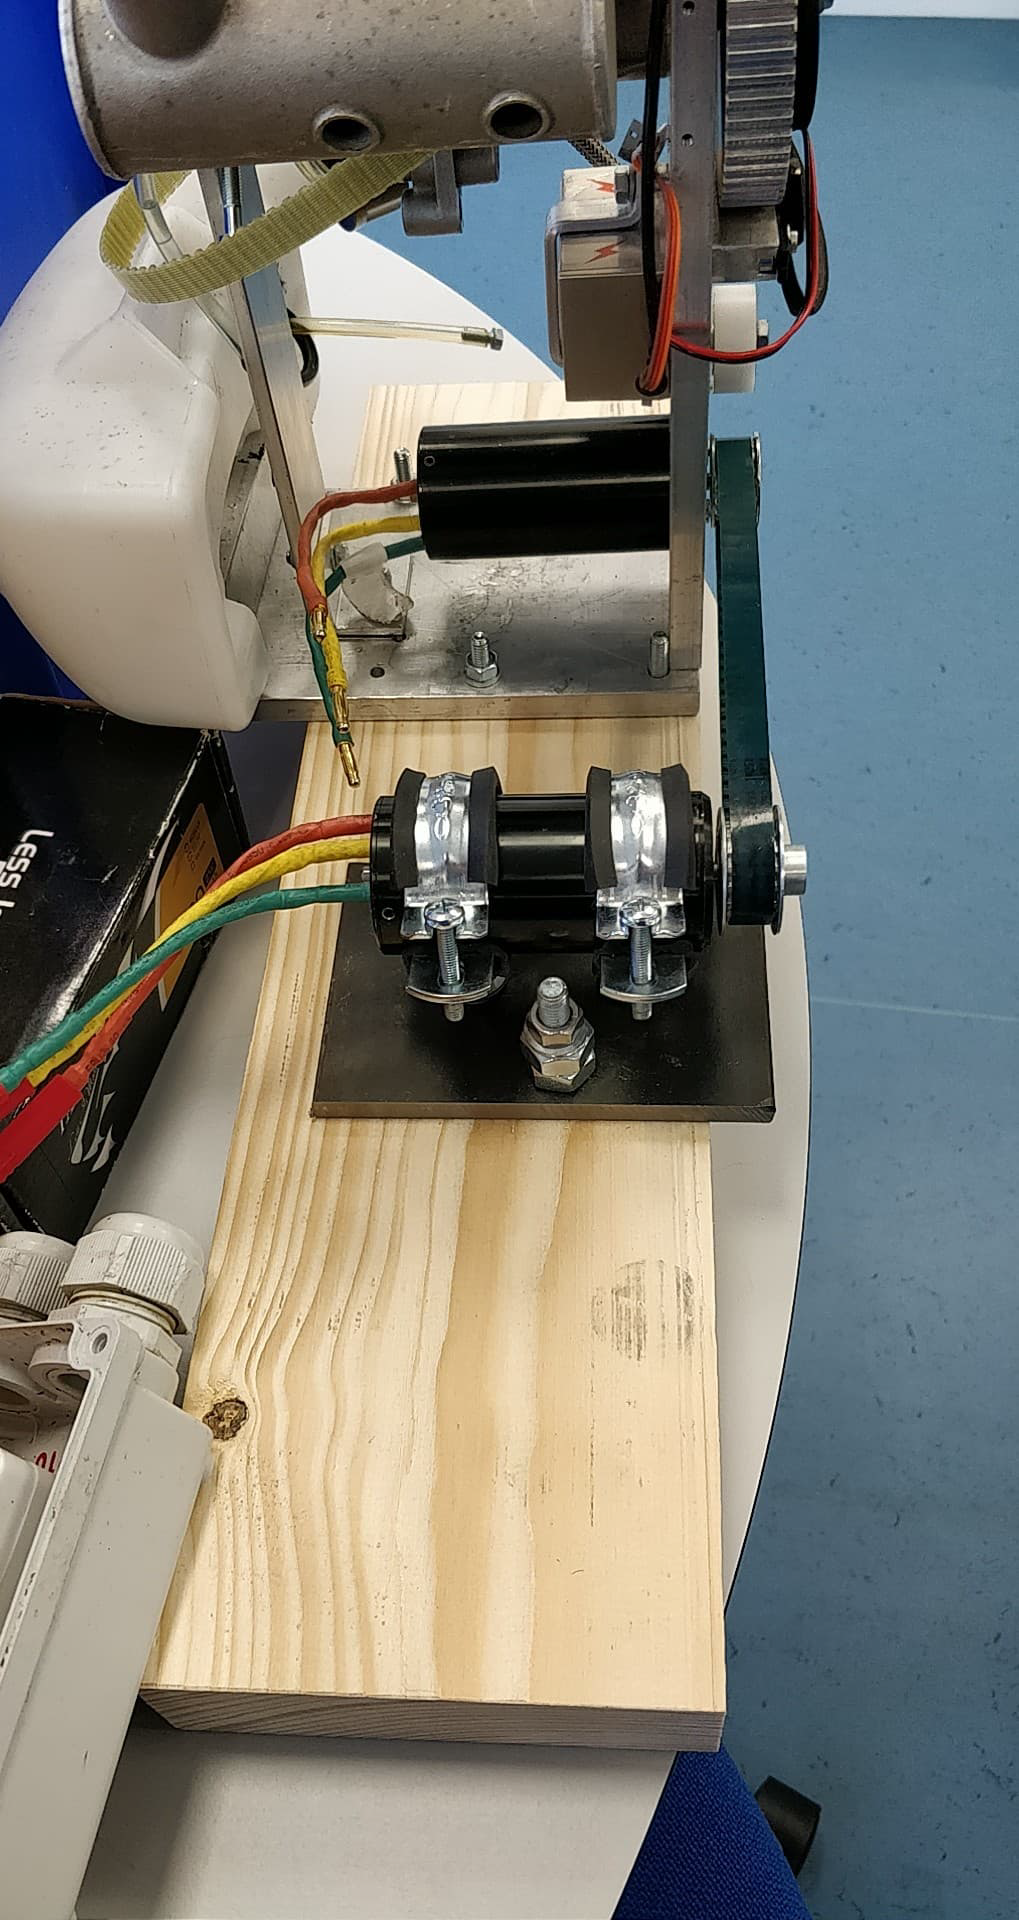
\includegraphics[width=0.3\textwidth]{./figurer/nt1.png}
  \caption{Foto af teststand til produktion af tre-faset spænding.}
  \label{fig:nt1}
\end{figure}

\begin{figure}[h]
  \centering
  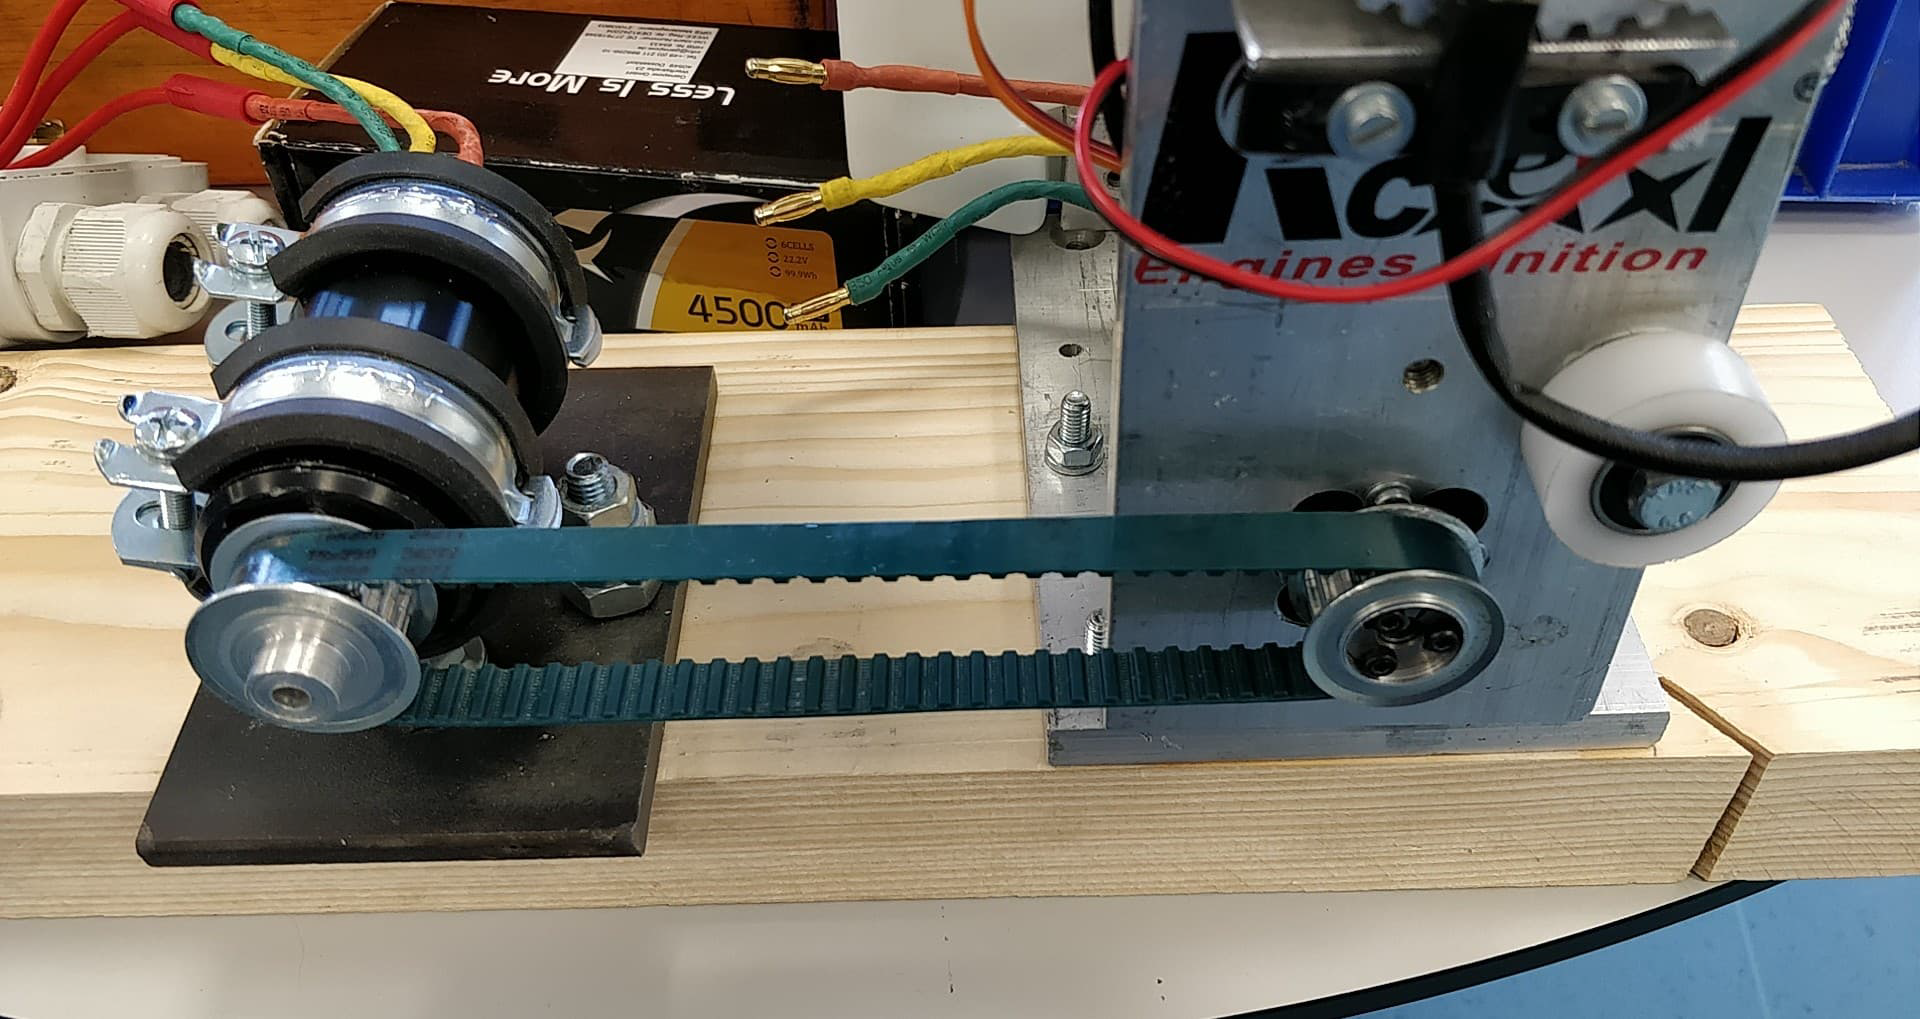
\includegraphics[width=0.6\textwidth]{./figurer/nt2.png}
  \caption{Foto af teststand til produktion af tre-faset spænding.}
  \label{fig:nt2}
\end{figure}

Ved hjælp af den tidligere benyttede ESC, vil det nu være muligt at starte den drivende motor med forskellige frekvenser, hvilket vil give et tilsvarende output på den nye generator. Dette output kan tilkobles den aktive ensretter, således at det er muligt at teste dens funktionalitet uden forbrændingsmotoren. 

Denne teststand blev benyttet til at producere en tre-faset spænding under samtlige test af den aktive ensretter.

\subsection{Realisering på breadboard (nedskaleret)}
\label{sec:real-pa-breadb}

Kredsløbet blev opbygget på et breadboard i en nedskaleret version for at teste funktionaliteten. Med nedskaleret menes der, at vi benyttede en 1 k$\Omega$’s modstand som load, således at der ikke blev trukket en stor strøm gennem kredsløbet. Der blev ligeledes påsat en tilpasset kondensator parallelt med load-modstanden for at udjævne eventuelt \textit{ripple} på outputtet. 

Figur \ref{fig:prens7} viser et skærmbillede fra målingen med oscilloskop af den nedskalerede realisering.

\begin{figure}[h]
  \centering
  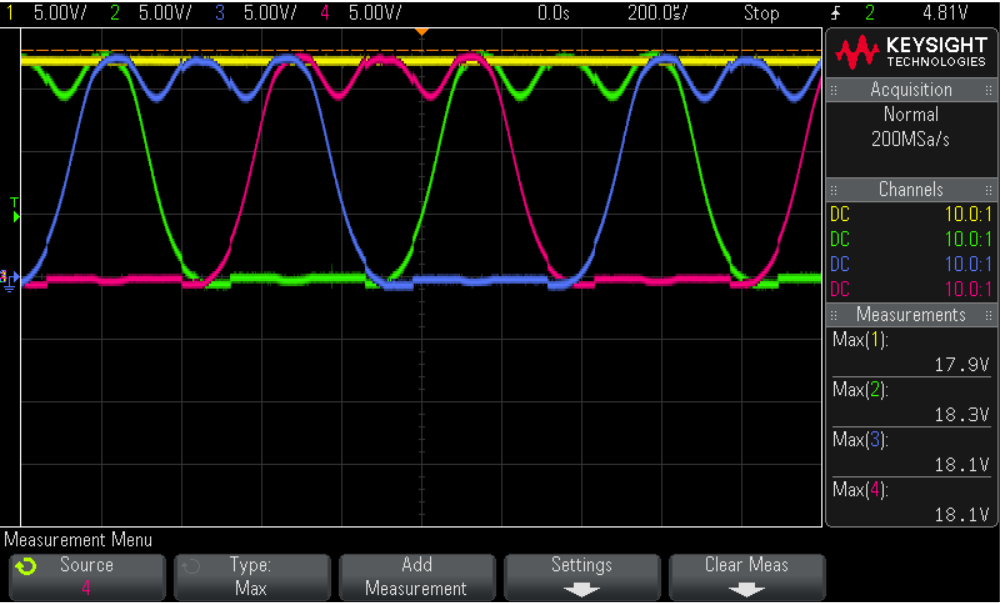
\includegraphics[width=0.5\textwidth]{./figurer/prens7.png}
  \caption{Nedskaleret realisering på breadboard. Gul: $V_{out}$. Grøn, blå og rød: $V_{in}$ (3 faser)}
  \label{fig:prens7}
\end{figure}

Her ses det, at outputtet er jævnt ensrettet i forhold til de tre faser, hvorved vi kunne konstatere, at det nedskalerede kredsløb fungerede efter hensigten.

Der er dog et spændingstab fra input til output på maks. 400 mV, hvilket er en tydelig forbedring ift. en passiv diodebro. Spændingstabet er forårsaget af MOSFET transistorens \textit{on resistance}, $R_{DS(on)}$, som under denne test var 4$\Omega$. Når kredsløbet skal realiseres uden nedskalering, vil der blive valgt en MOSFET med en langt mindre $R_{DS(on)}$, hvilket teoretisk vil forbedre kredsløbet yderligere\footnote{Se bilag, Timebox 7, for yderligere information.}.  



% For yderligere at bevise, at den aktive ensretter var væsentlig mere effektiv end en standard diodebro, foretog vi en måling af spændingen på én af MOSFET transistorernes gate pin i forhold til fasen på transistorens \textit{source} pin.

% Figur \ref{fig:prens8} viser et skærmbillede af resultatet af målingen. 

% \begin{figure}[h]
%   \centering
%   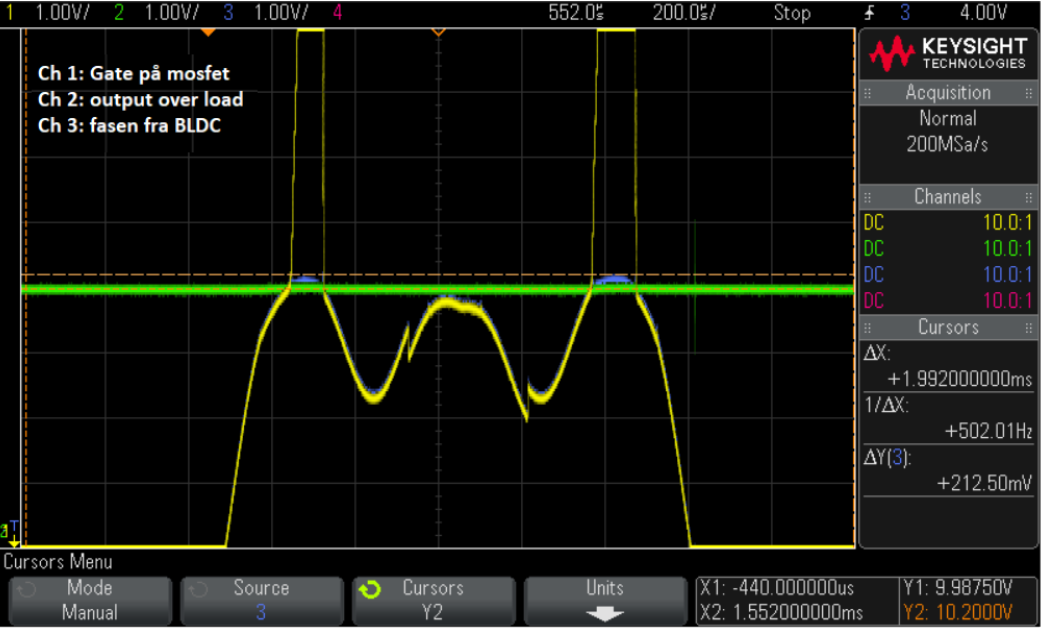
\includegraphics[width=0.5\textwidth]{./figurer/prens8.png}
%   \caption{Måling af gate- vs. source spænding}
%   \label{fig:prens8}
% \end{figure}

% Her ses det, at der er et spændingsfald på 212.5 mV fra gate til source, hvilket er en klar forbedring i forhold til en diodes forward spænding på 700 mV.

% Spændingstabet er forårsaget af MOSFET transistorens on resistance, RDS(on), som under denne test var 4$\Omega$. Når kredsløbet skal realiseres uden nedskalering, vil der blive valgt en MOSFET med en langt mindre RDS(on), hvilket teoretisk vil forbedre kredsløbet yderligere.\footnote{Se bilag, Timebox 7, for yderligere information}

\subsection[PDB print]{PCB print\protect\footnote{Se bilag, Timebox 8, for yderligere information.}}
\label{sec:pcb-printf-bilag}

Under realiseringen af den nedskalerede version af kredsløbet, fik vi konstateret, at kredsløbet havde den ønskede funktionalitet, hvorfor vi designede et PCB print med programmet, Eagle. Da printet var færdigt, blev følgende komponenter loddet på:

\begin{itemize}
\item 6 stk. MOSFET transistorer.
  \begin{itemize}
  \item Fairchild, FDP61N20, N-channel\footnote{Datasheet: http://213.114.131.21/_pdf/FD/FDP61N20.pdf}.
  \item Max drain strøm: 61 A.
  \item Max drain-source spænding: 200 V.
  \item $R_{DS(on)}$: 41 m$\Omega$.
  \item $R_{thJA}$: 62.5 $^\circ$C/W
\end{itemize}
\item 6 stk. 100 k$\Omega$’s modstande (1\% tolerance).
\item 9 stk. dioder, 1N4148.
\item 3 stk. IC, LT4320-1 
\end{itemize}

Figur \ref{fig:nt3} og \ref{fig:nt4} viser et skærmbillede af det færdige PCB print.

\begin{figure}[h]
  \centering
  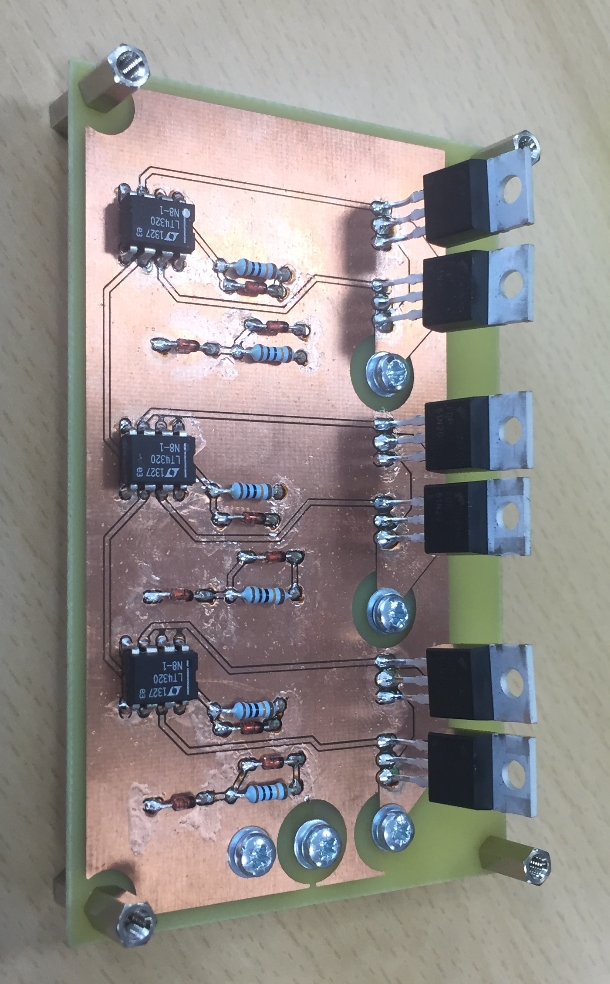
\includegraphics[angle=90,width=0.5\textwidth]{./figurer/nt3.png}
  \caption{PCB print. Top lag}
  \label{fig:nt3}
\end{figure}

\begin{figure}[h]
  \centering
  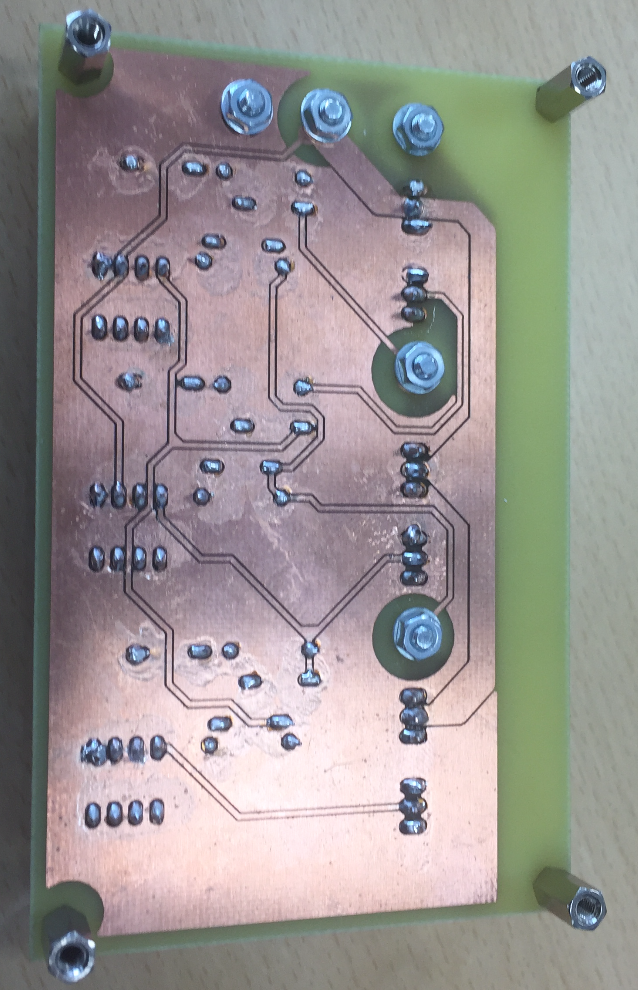
\includegraphics[angle=90,width=0.5\textwidth]{./figurer/nt4.png}
  \caption{PCB print. Bund lag}
  \label{fig:nt4}
\end{figure}


\subsection[Implementering]{Implementering\footnote{Se bilag, Timebox 9-10, for yderligere information.}}
\label{sec:result-bilag-timeb}

Efter konstruktionen af PCB printet til den aktive ensretter, var det tid til at teste kredsløbet \textit{full scale}. Indledningsvist besluttede vi os dog for at lave en nedskaleret test på samme måde som på breadboardet. Altså med en load-modstand på 1 k$\Omega$.

\subsubsection{Nedskaleret test af PCB}
\label{sec:nedskaleret-test-af}

Figur \ref{fig:nt5} og \ref{fig:nt6} viser resultatet af den nedskalerede test af PCB printet.
\clearpage
\begin{figure}[h]
  \centering
  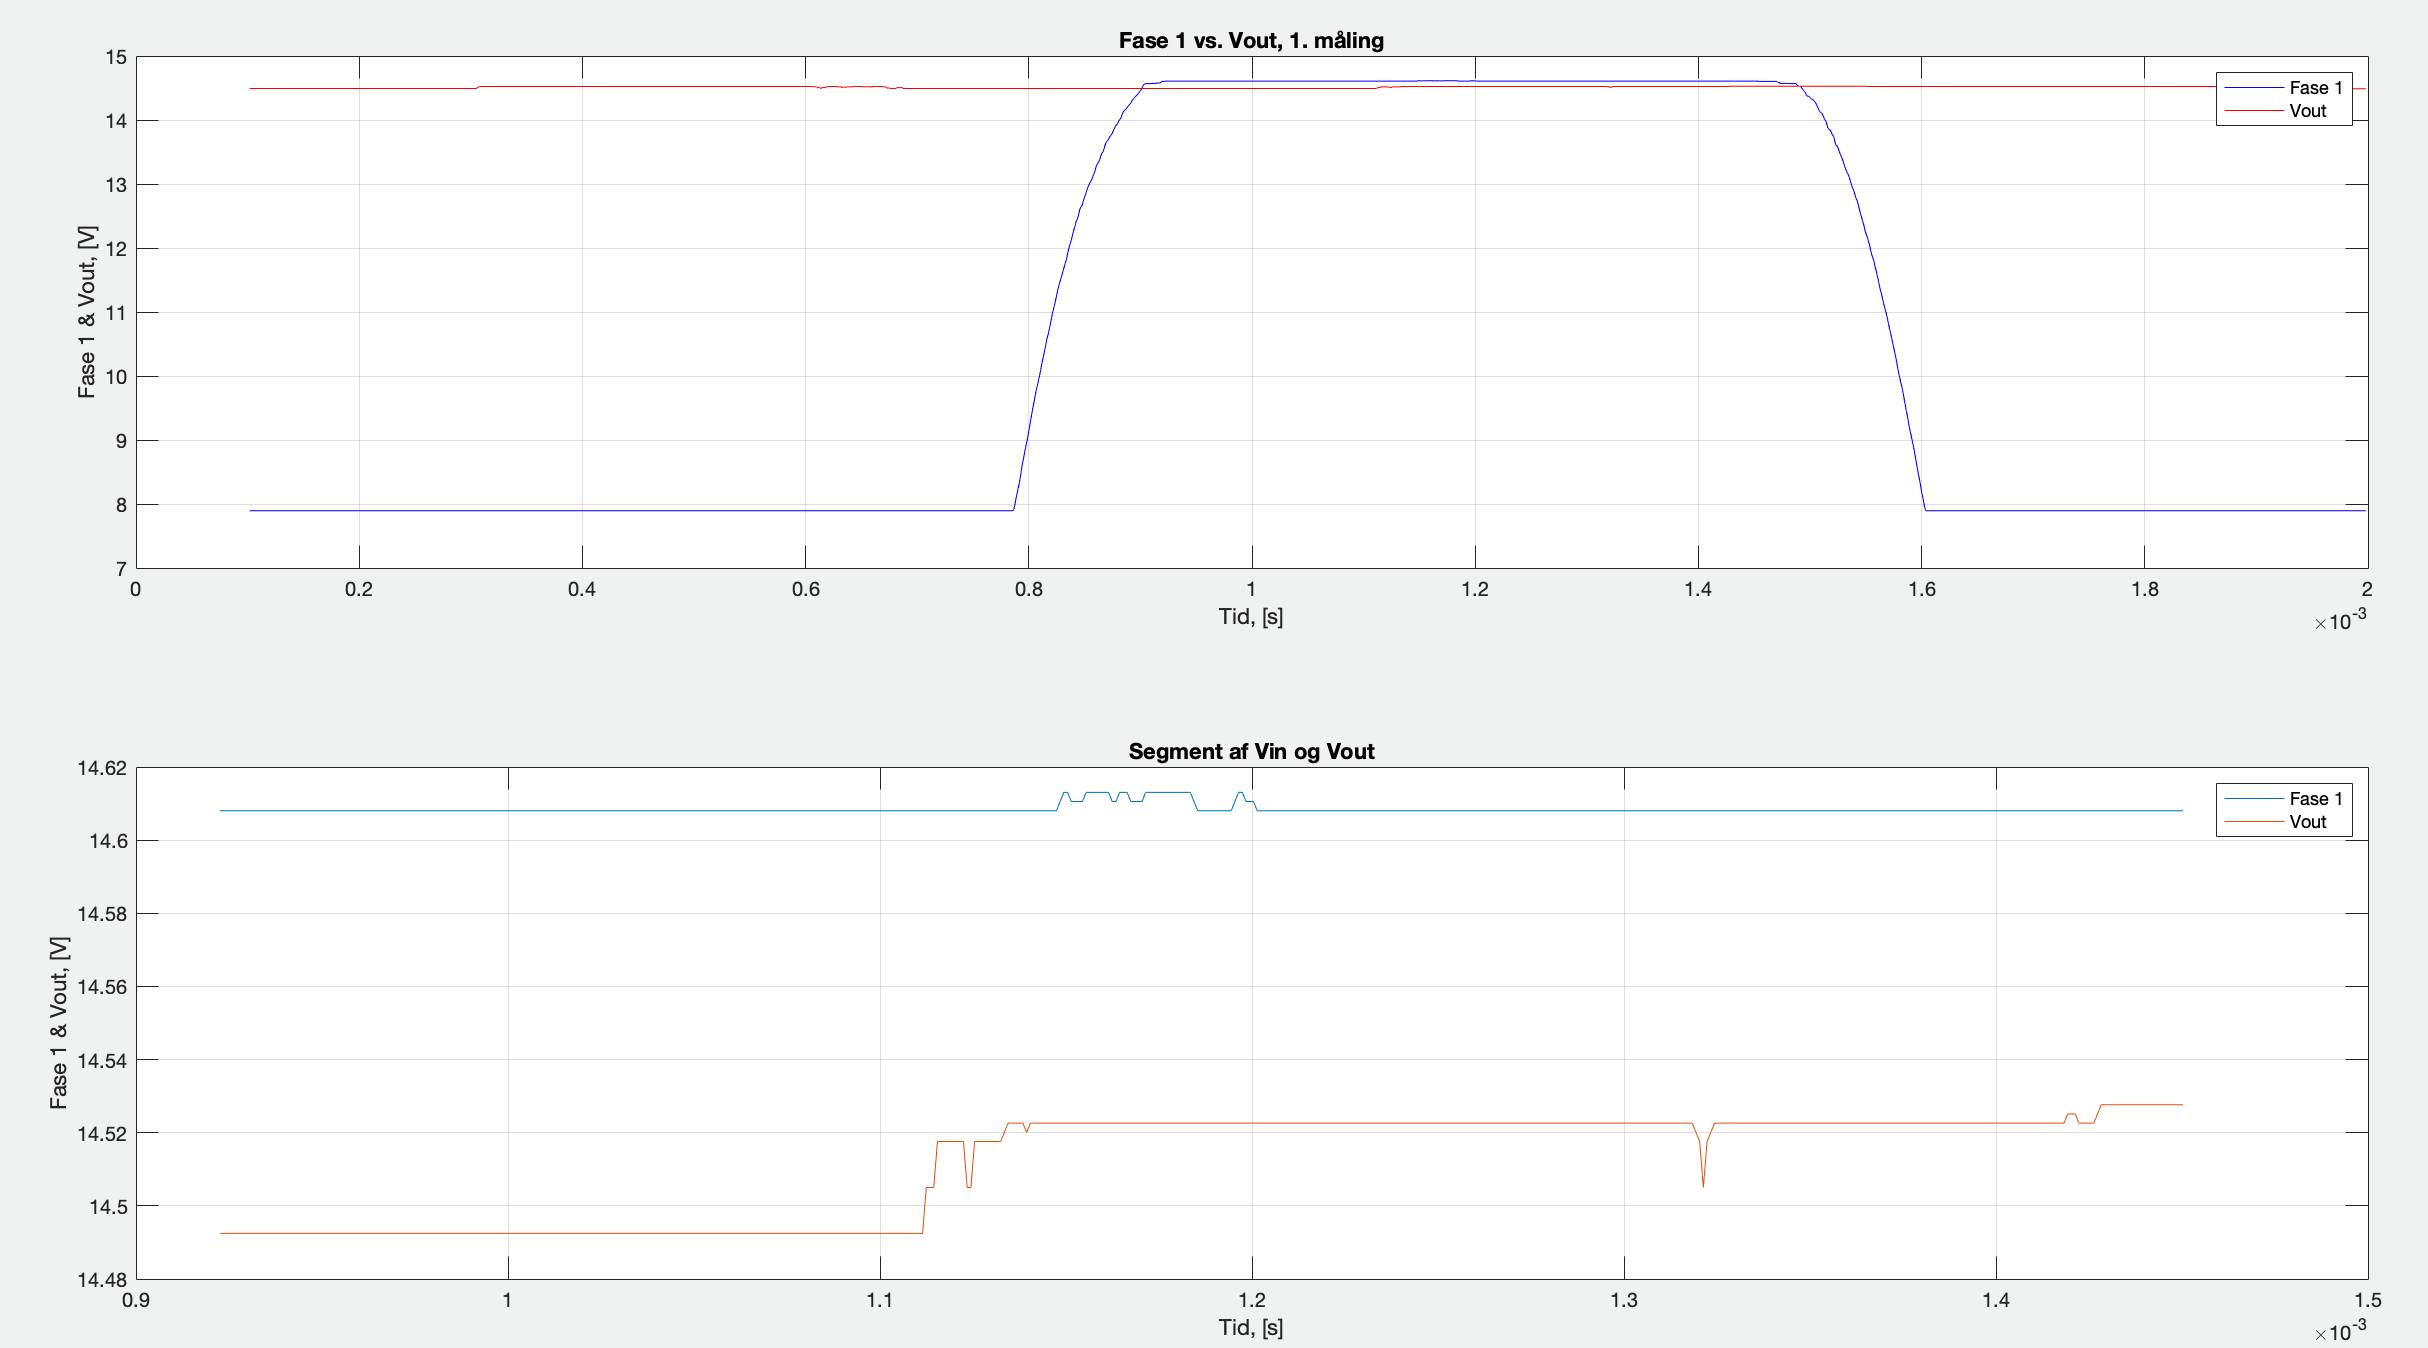
\includegraphics[width=0.5\textwidth]{./figurer/nt5.png}
  \caption{Første måling ($V_{in}$ = 14.613 V, $V_{out}$ = 14.528 V)}
  \label{fig:nt5}
\end{figure}

\begin{figure}[h]
  \centering
  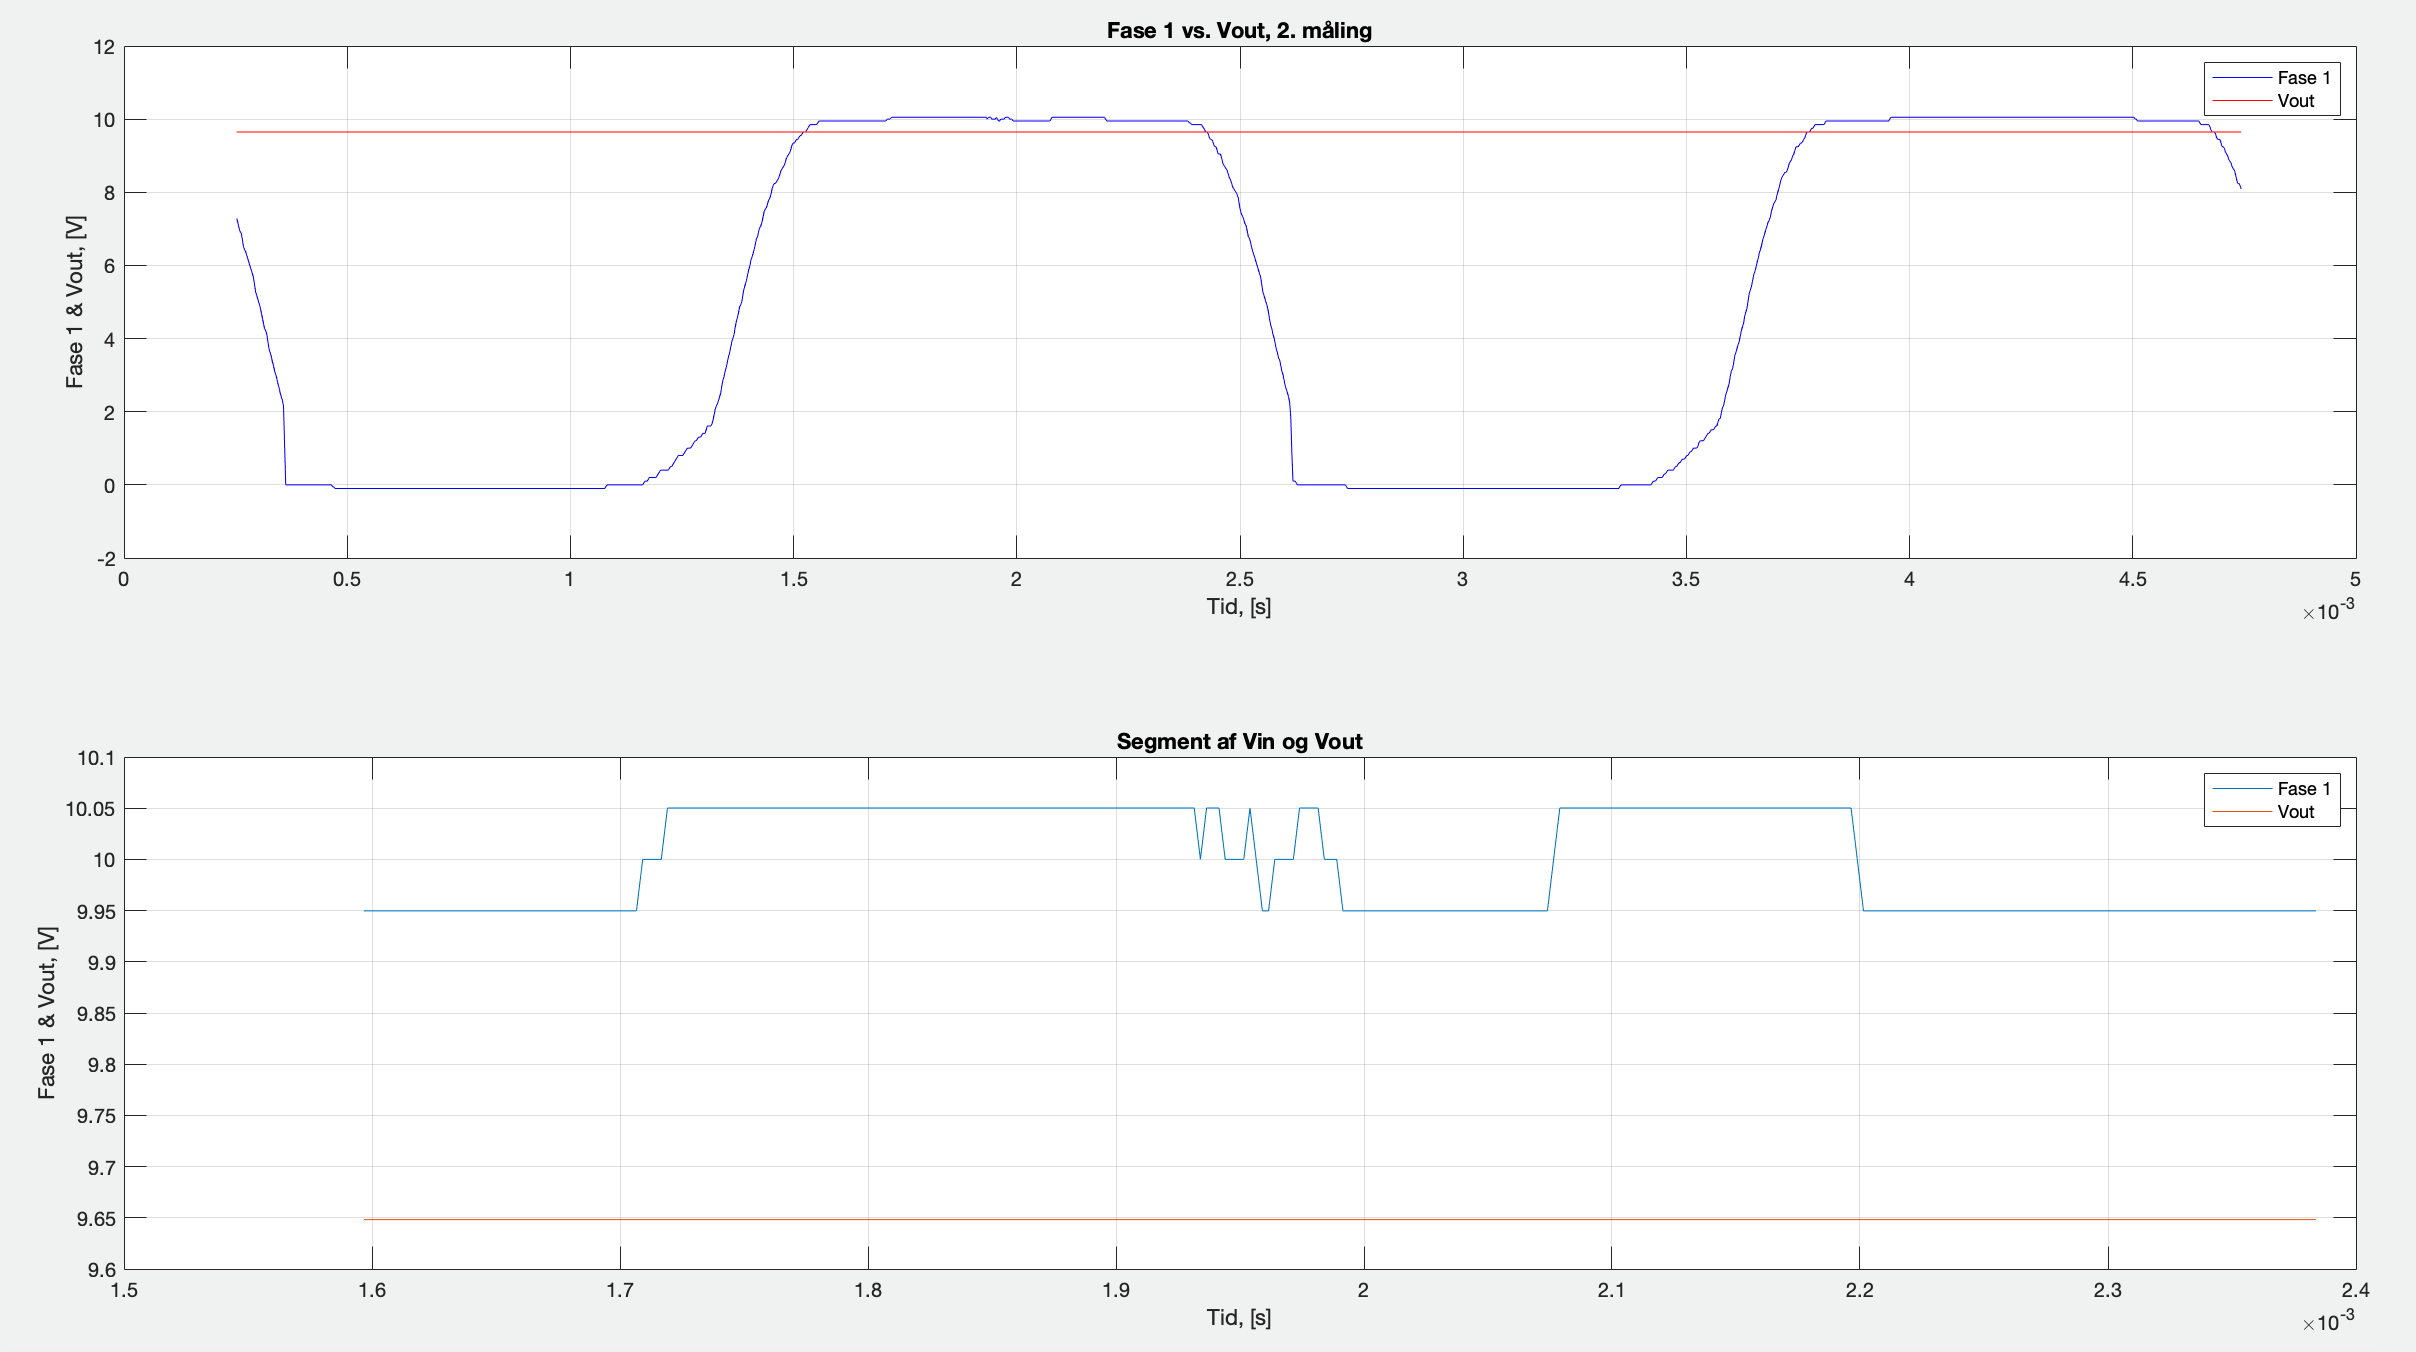
\includegraphics[width=0.5\textwidth]{./figurer/nt6.png}
  \caption{Anden måling ($V_{in}$ = 10.050 V, $V_{out}$ = 9.648 V)}
  \label{fig:nt6}
\end{figure}

Som det ses ud fra begge plots i figur \ref{fig:nt5} og \ref{fig:nt6}, er der et spændingstab på udgangen af ensretteren i forhold til indgangen. Spændingstabene for målingerne er i Matlab udregnet til:

\begin{tabular}{p{2cm}l}
  1. måling: &$V_{delta1}$ = 0.0967 volt.\\
  2. måling: &$V_{delta2}$ = 0.3497 volt.\\
\end{tabular}

Printet ser ud til at have den ønskede funktionalitet. Der ses dog en ujævnhed i spændingstabet gennem kredsløbet i de to målinger, hvilket vi ikke umiddelbart kan forklare.


\subsubsection{Større load}
\label{sec:storre-load}

For at teste om kredsløbet kunne leve op til de store strømme (ca. 80 A peak), som det færdige HPP system teoretisk set kan komme til at trække, blev der anskaffet en effektmodstand på ca. 12 m$\Omega$, se figur \ref{fig:nt7}. Denne effektmodstand kan håndtere op til 25 A. Kredsløbet kan ikke testes fuldt ud med denne modstand, men det vil give en indikation af, hvordan kredsløbet reagerer ved en større belastning.
\clearpage
\begin{figure}[h]
  \centering
  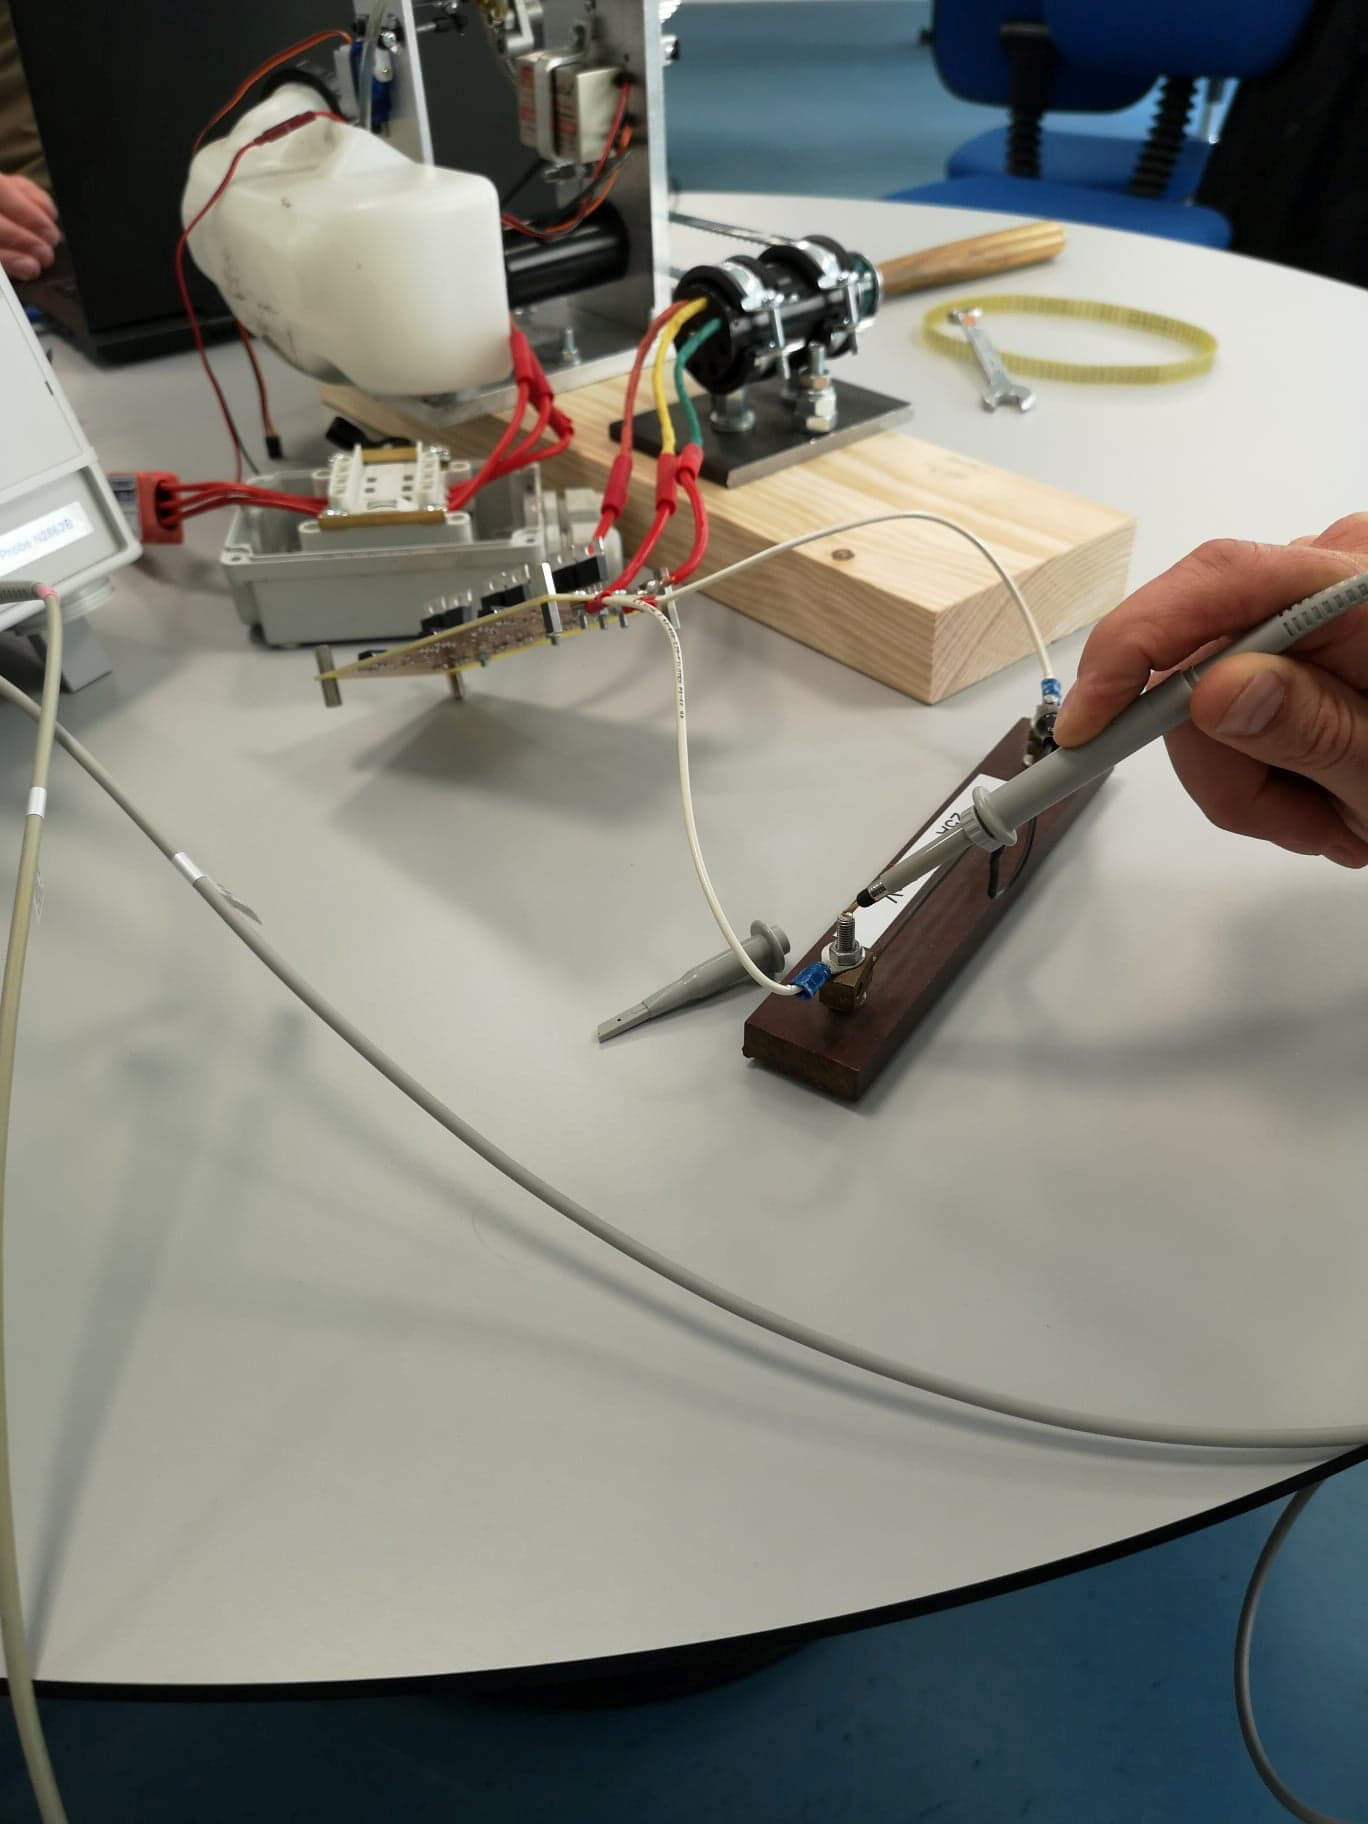
\includegraphics[width=0.5\textwidth]{./figurer/nt7.png}
  \caption{Foto af testopstilling med load modstand på 12 m$\Omega$.}
  \label{fig:nt7}
\end{figure}

Effektmodstanden er designet således, at der løber 25 A gennem den, hvis der er et spændingsfald på 300 mV over modstanden.

\begin{tabular}{p{2cm}l}
  1. måling: &Generatoren blev drevet således, der løb ca. 25 A gennem load modstanden.\\
\end{tabular}

Efter få sekunder kunne vi konstatere, at de seks MOSFET transistorer på printet blev meget varme, hvorfor testen blev stoppet.

Hvis det antages, at der i værste fald er et spændingsfald på de tidligere beregnede 0.3497 V fra source til drain på hver af de 6 transistorer, vil dette resultere i et effekttab på:

\begin{equation}
  \label{eq:2}
  P = \frac{0.3497^2V}{0.041 \Omega}=2.87 W
\end{equation}

Og dette vil aflede en stigning i temperaturen i transistorerne på:

\begin{equation}
  \label{eq:3}
  T=P\cdot R_{thJA} = 2.87 W \cdot 62.5 \frac{^\circ C}{W}=179.2 ^\circ C
\end{equation}

Ud fra datasheet’et til FDP61N20 ses det, at de maksimalt kan håndtere 150 $^\circ C$. Vi var derfor nødt til enten at finde nye transistorer med en lavere intern modstand og/eller påmontere en \textit{heatzink}. Vi blev efter denne test ligeledes bekymret for, at kredsløbet ikke fungerede optimalt, da vi begyndte at se en del uregelmæssigheder.

\subsubsection{Fejlsøgning}
\label{sec:fejlsogning}

Indledningsvist blev der indkøbt følgende MOSFET transistorer med en lavere intern modstand:

\begin{itemize}
\item $OptiMOS^{TM}5$ Power-transistor
  \begin{itemize}
  \item Max drain strøm: 100 A.
  \item Max drain-source spænding: 100 V.
  \item $R_{DS(on)}$: 3.9 m$\Omega$.
  \item $R_{thJA}$: 62 $^\circ$C/W
  \end{itemize}
\end{itemize}

Disse MOSFET transistorer blev monteret på PCB printet, hvorefter samme testprocedure som tidligere blev gennemført.  

Testen resulterede dog i en defekt transistor.

\begin{figure}[h]
  \centering
  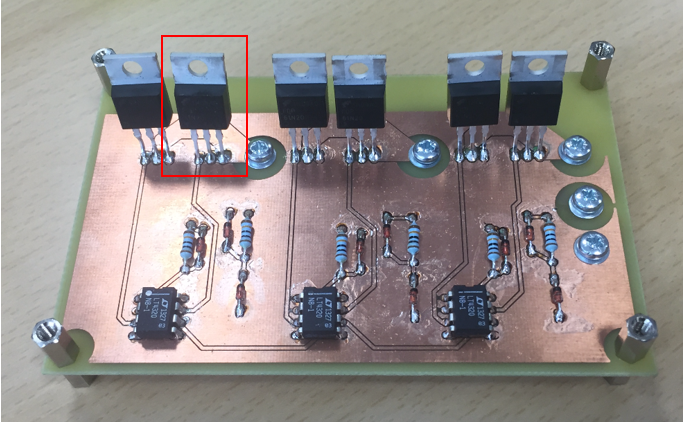
\includegraphics[width=0.5\textwidth]{./figurer/nt8.png}
  \caption{Defekt transistor. Markeret med rød firkant.}
  \label{fig:nt8}
\end{figure}

Årsagen til defekten var på daværende tidpunkt uafklaret, hvorfor det blev besluttet at måle gate spændingerne på samtlige transistorer i forhold til stel, da vi havde en mistanke om, at der var ubalance i kredsløbet. Ubalance kunne muligvis være årsagen til defekten af den ene transistor. 

Figur \ref{fig:nt9} viser målingen af gate spændingen på de tre transistorer, der håndterer den positive del af inputtet. Hvis kredsløbet fungerede korrekt, skulle der gerne være samme spændingsniveau på samtlige \textit{gates}. 

\begin{figure}[h]
  \centering
  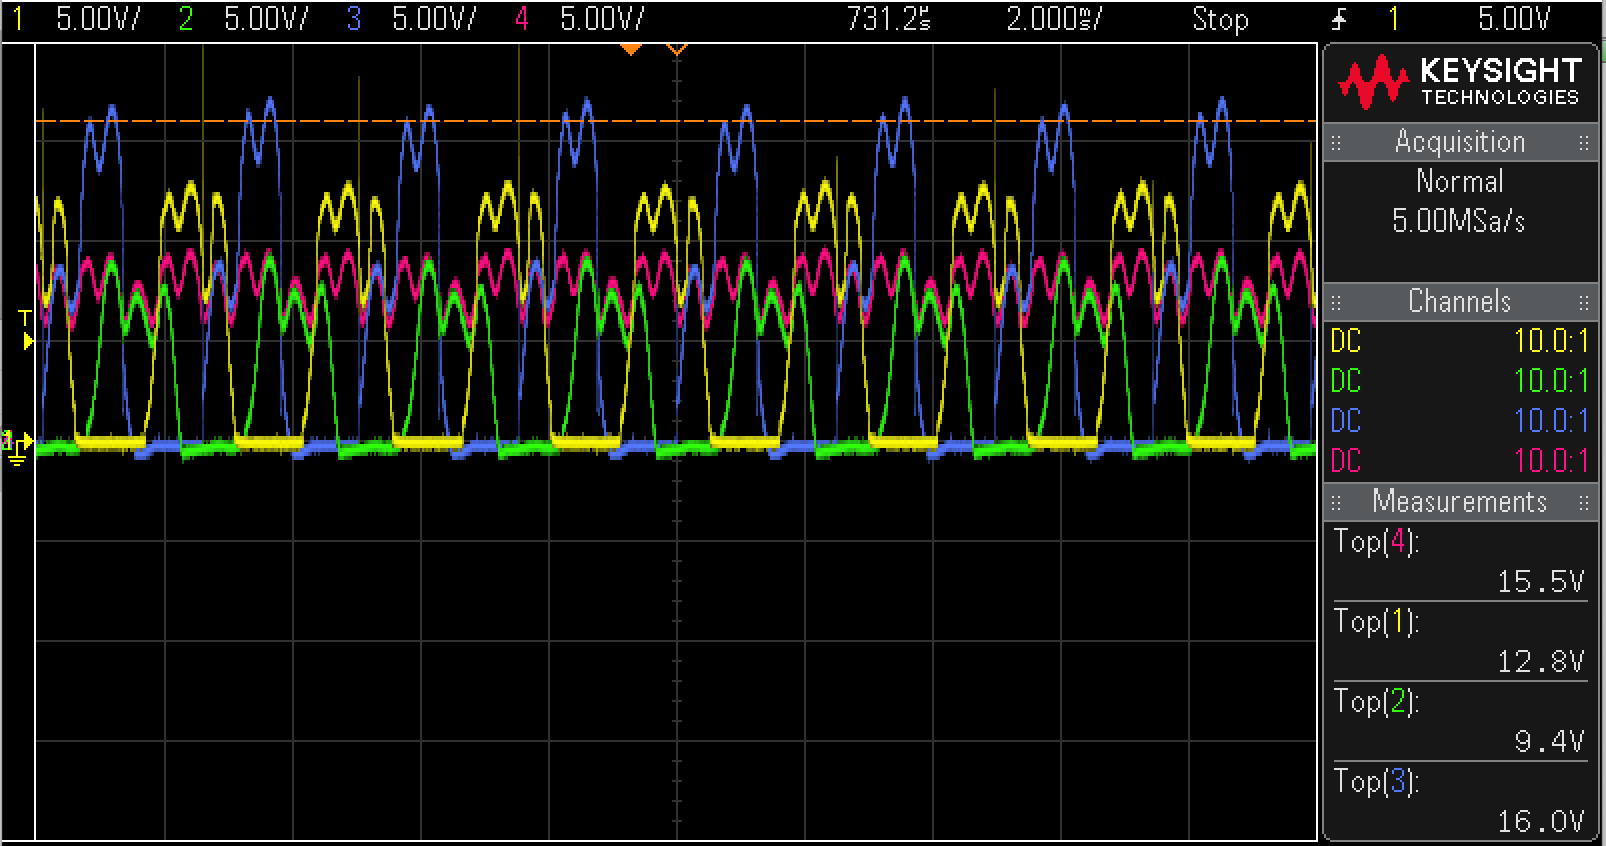
\includegraphics[width=0.5\textwidth]{./figurer/nt9.png}
  \caption{Gatespænding. Grøn: fase 1+, blå: fase 2+, gul: fase 3+, rød: $V_{out}$}
  \label{fig:nt9}
\end{figure}

Her ses, at gate spændingerne ikke har samme niveau. Peak værdier varierer mellem 9.4 V (fase 1), 12.8 V (fase 2) og 16.0 V (fase 3). På baggrund af denne måling, og da vi ikke havde mere tid til rådighed, var vi desværre nødsaget til at stoppe udviklingen af den aktive ensretter. 


\section{Spændingsregulator (Jacob)}
\label{sec:spand-jacob}

\subsection{Analyse af LM78xx-serien}
\label{sec:analyse-af-lm78xx}

Én af mulighederne for at lave en spændingsregulator er, at bruge en LM7805 IC til opgaven. Fordelen ved en implementering af denne type er, at spændingsregulatoren er simpel, billig og kan laves på meget lidt plads. Ét af de problemer man kan støde på under spændingsreguleringen, er temperaturforøgelse, der kan brænde komponenten af. Bruges der blot en LM7805 til at regulere fra 22 V til 5 V, med en strøm på 1 A, vil der være et effekttab på 17 W.\footnote{Effekten fås ved $P=V\cdot A$}

Af dataarket for LM7805\footnote{(FAIRCHILD, 2006)} opgives det, at temperaturforøgelsen i IC’en er 65 $^\circ C/W$ der forbruges i IC’en. Altså vil vi, udregnet i grader, få en temperaturforøgelse på:

\begin{equation}
  \label{eq:3}
  \Delta T = I \cdot \Delta V \cdot R_{\theta (JA)}=1 A \cdot (22V-5V)\cdot 65 \frac{^\circ C}{W} = 1105^\circ C
\end{equation}

En sådan temperaturstigning er selvfølgelig langt fra acceptabel.

Monteres der en heatsink i de passende dimensioner, falder $R_{\theta J}$ til 5 $\frac{^\circ C}{W}$. Dermed ser beregningen således ud: 

\begin{equation}
  \label{eq:3}
  \Delta T = I \cdot \Delta V \cdot R_{\theta (JA)}=1 A \cdot (22V-5V)\cdot 5 \frac{^\circ C}{W} = 85^\circ C
\end{equation}

Dette er indenfor et acceptabelt område, da $T_{OPR} \in  [-40 ^\circ C;125 ^\circ C]$. Dog skal det nævnes, at temperatursvingningerne er den største udfordring for holdbarheden på en IC. Endvidere vil det forøge størrelsen og vægten af systemet meget væsentligt.

Hvad angår strømmen kan LM78xx serien klare op til 2,2 A peak og levere en outputstrøm på op til 1 A. Da vores krav var 1 A på udgangen, går serien lige an, hvad angår strømstyrke. Denne type af system er altså yderst ineffektivt, da der afsættes en stor mængde energi til termisk energi. Problemerne med holdbarheden på IC’erne kan løses ved at sætte to forskellige IC’er i serie. Eksempelvis kunne der laves et system som det, der vises i figur \ref{fig:j2}. Det løser dog ikke problemerne med ineffektivitet, hvorfor denne mulighed afskrives allerede efter analysefasen.

\begin{figure}[h]
  \centering
  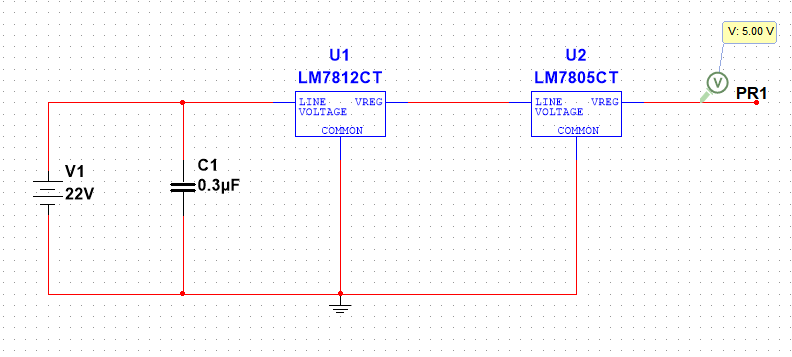
\includegraphics[width=0.7\textwidth]{./figurer/j2.png}
  \caption{Eksempel på system}
  \label{fig:j2}
\end{figure}

\subsection{Analyse af LM317 }
\label{sec:analyse-af-lm317}

I figur \ref{fig:j3} ses en simulering af opsætningen af en spændingsregulator på baggrund af en LM117. Opstillingen er lavet på baggrund af en af standardopstillingerne i datasheetet for LM117/LM317T.\footnote{(TI, 2018)}

\begin{figure}[h]
  \centering
  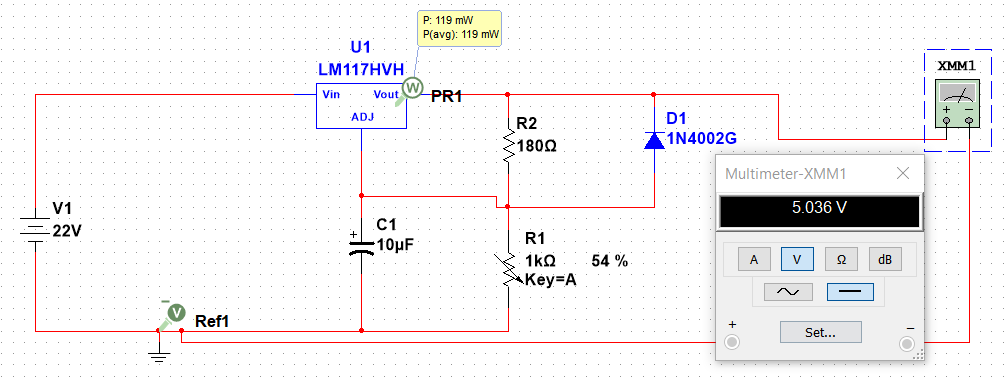
\includegraphics[width=0.7\textwidth]{./figurer/j3.png}
  \caption{Diagram til simulering}
  \label{fig:j3}
\end{figure}

Som det ses af simuleringen, opnås den ønskede spænding, og den effekt der afsættes i LM117 er meget acceptabel. Dette effekttab vil give en temperaturstigning i LM117 på 22,1 grader, hvilket følger af de temperaturkarakteristika der gælder for LM117 iflg. dataarket. Ulempen ved denne løsning er, at den er væsentligt dyrere end en løsning der bygger på LM78xx-serien.

\subsection{Analyse af BUCK-konverter}
\label{sec:analyse-af-buck}

En anden mulighed for konvertering af spændingen er med en BUCK converter. Opstillingen i figur \ref{fig:j4} kommer fra et designværktøj udviklet af Texas Instruments, kaldet WEBENCH.\footnote{(Instruments, 2019)}

I nævnte værktøj indtastes blot den ønskede input og outputstrøm og spænding, hvorefter der tegnes forskellige mulige kredsløb, som man kan vælge imellem. På baggrund af effektivitet og kostpris, valgtes følgende. 

\begin{figure}[h]
  \centering
  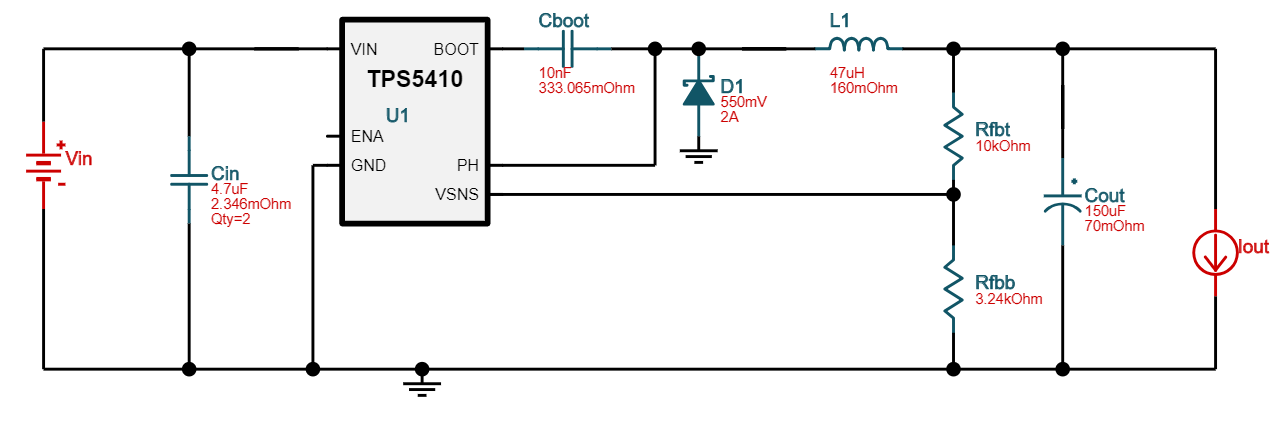
\includegraphics[width=0.7\textwidth]{./figurer/j4.png}
  \caption{WEBBENCH}
  \label{fig:j4}
\end{figure}

Værktøjet indeholder også et analyseværktøj. For at bekræfte, at kredsløbet giver den ønskede outputspænding, er  karakteristikken i steady state undersøgt.
\clearpage
\begin{figure}[h]
  \centering
  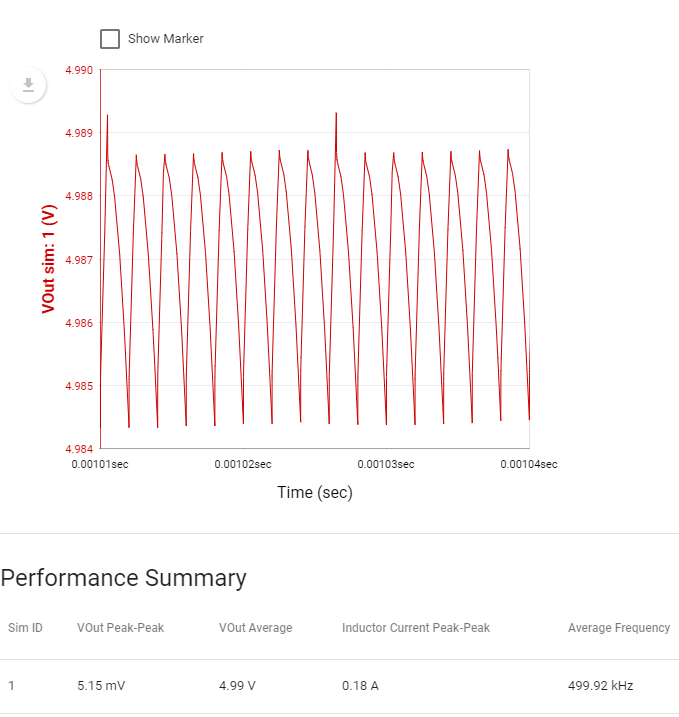
\includegraphics[width=0.7\textwidth]{./figurer/j5.png}
  \caption{Måling af spænding}
  \label{fig:j5}
\end{figure}

Som det ses af figur \ref{fig:j5}, opnås den ønskede spænding. Billedet viser en del ripple, men denne er underordnet, så længe den ikke har større udsving end det vises her. Effektiviteten for ovenstående konverter er på 86,1\%, og effekttabet i IC'en udregnes af programmet til 208 mW. Dette giver, i forhold til de i dataarket oplyste temperaturkarakteristika, en temperaturstigning på 22,02 grader, hvilket er acceptabelt, også uden heatsink. Endvidere er denne løsning væsentlig billigere da ét styk TPS5410DR kan erhverves for cirka 20 kr. 

Efter analysen kan det konkluderes, at LM78xx-serien er en ineffektiv og ringe løsning til HPP. På baggrund af analyse og simulering af LM317 og BUCK-konverteren kan det ikke afgøres, hvilken opsætning der er bedst i HPP. Derfor bygges begge systemer på breadboard, for at teste dem.

\subsection{Implementering af LM317}
\label{sec:impl-af-lm317}

I figur \ref{fig:j6} ses opstillingen realiseret. 
\clearpage
\begin{figure}[h]
  \centering
  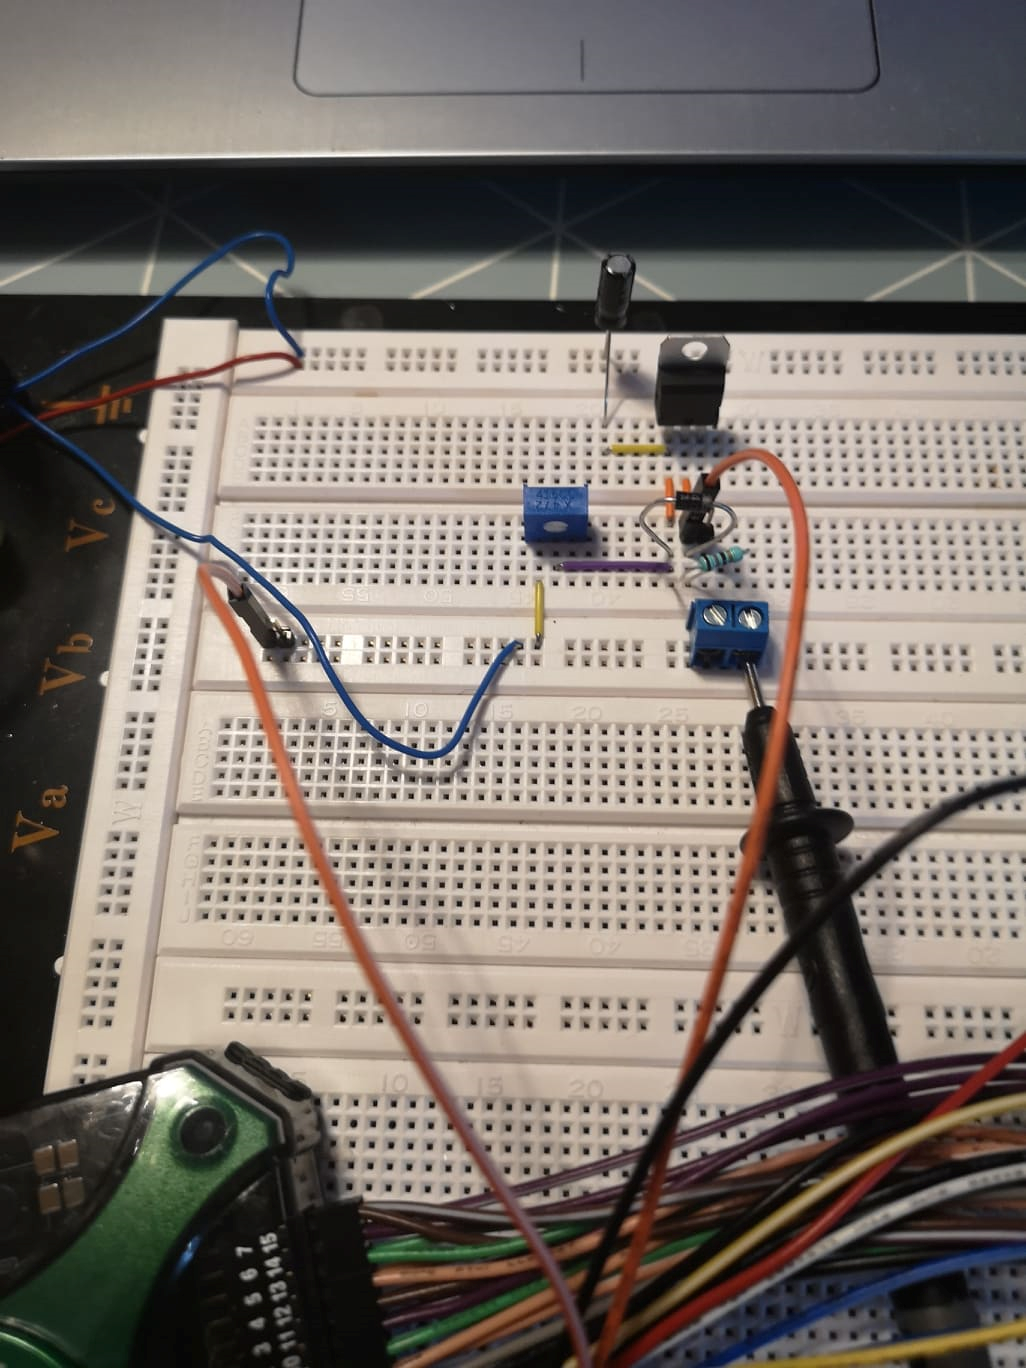
\includegraphics[width=0.35\textwidth]{./figurer/j6.png}
  \caption{Opstilling realiseret}
  \label{fig:j6}
\end{figure}


Som det også ses af billedet har opstillingen en meget beskeden størrelse og vægt, hvilket er en stor fordel for vores vedkommende, som det også fremgår af de overordnede krav for projektet. Prisen på alle komponenter er billig. Det dyreste er LM317 til cirka 11 kroner stykket. Samlet pris for hele systemet beløber sig til cirka 19 kroner. Efter første test, blev systemet udsat for varme, fra en lighter, for at se udsving.
\begin{figure}[h]
  \centering
  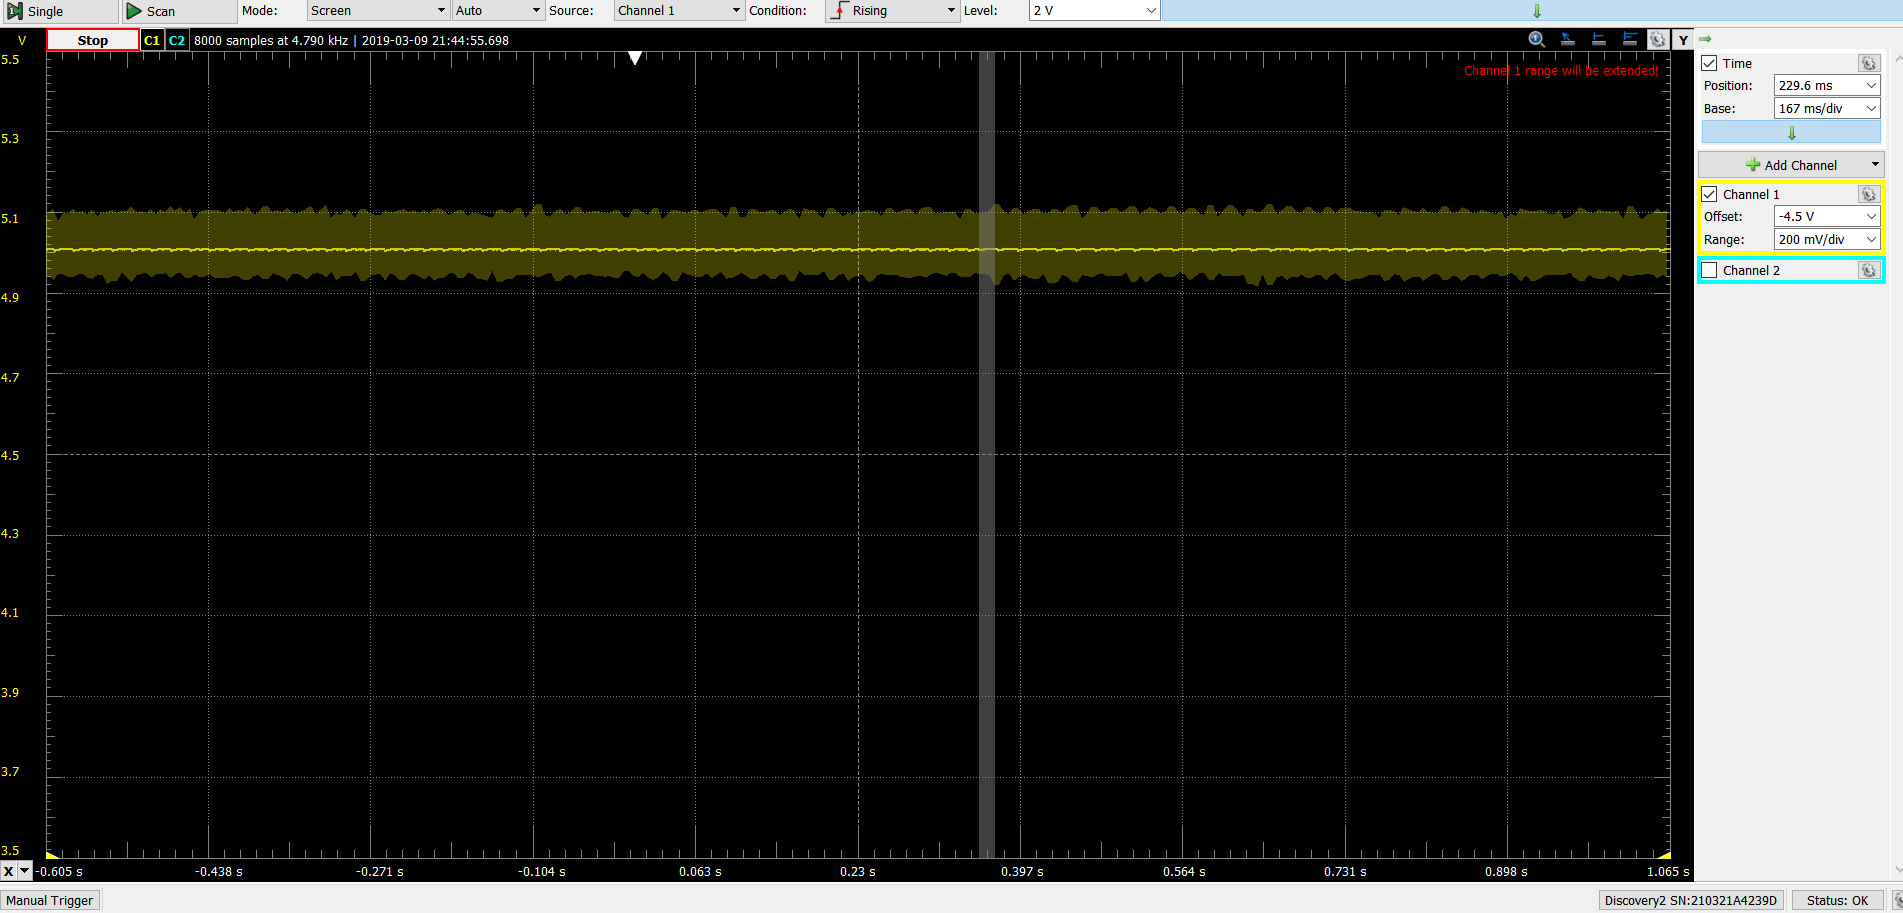
\includegraphics[width=0.7\textwidth]{./figurer/j7.png}
  \caption{LM317 output}
  \label{fig:j7}
\end{figure}

I figur \ref{fig:j7} ses outputtet fra LM317-systemet. Som vi kan se, ligger spændingen lige omkring 5 V som påkrævet. Selvom der ikke er zoomet voldsomt meget ind, ses også et acceptabelt niveau af ripple. Potentiometeret blev udmålt til 538 $\Omega$, hvilket også stemmer meget godt overens med vores simulering. Der blev målt en strøm på 1024 mA på systemet, hvilket kun er en smule over det krævede niveau. Efter datasheetet burde vi kunne opnå 1,5 A. Strømmen blev målt ved at forbinde regulatoren med en load-modstand.
\clearpage
\begin{figure}[h]
  \centering
  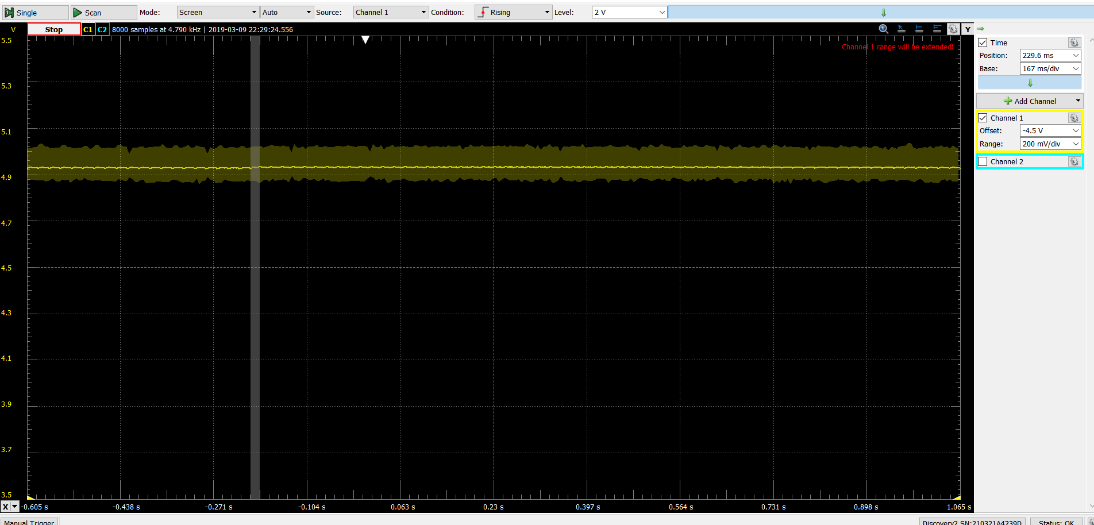
\includegraphics[width=0.7\textwidth]{./figurer/j8.png}
  \caption{Spænding efter varmeudsættelse}
  \label{fig:j8}
\end{figure}

I figur \ref{fig:j8} ses spændingen efter vi havde udsat systemet for lighteren i 30 sekunder. Spændingen falder en smule, men indenfor det acceptable, og ripple forøges ikke.

\subsection{Test af BUCK-konverteren}
\label{sec:test-af-buck}

I figur \ref{fig:j9} ses implementeringen af BUCK-konverteren. Ligesom med tidligere test, bliver systemet her også udsat for varme og en load-modstand. 

\begin{figure}[h]
  \centering
  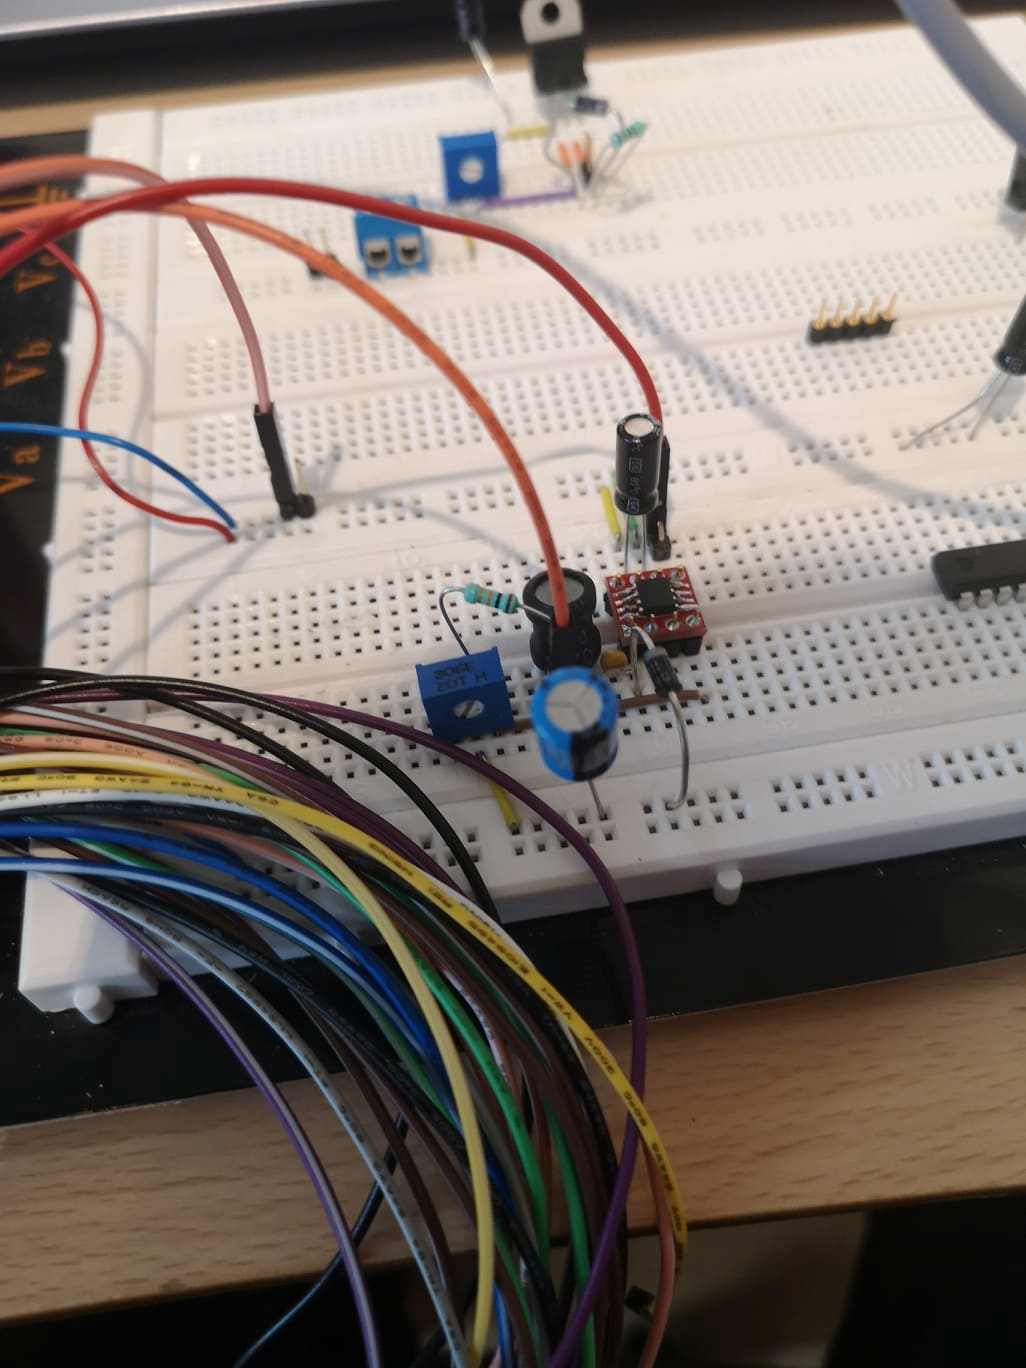
\includegraphics[width=0.35\textwidth]{./figurer/j9.png}
  \caption{Testopstilling af BUCK-konverter}
  \label{fig:j9}
\end{figure}
\clearpage
I figur \ref{fig:j10} ses resultater for testen. Først under almindelige omstændigheder.

\begin{figure}[h]
  \centering
  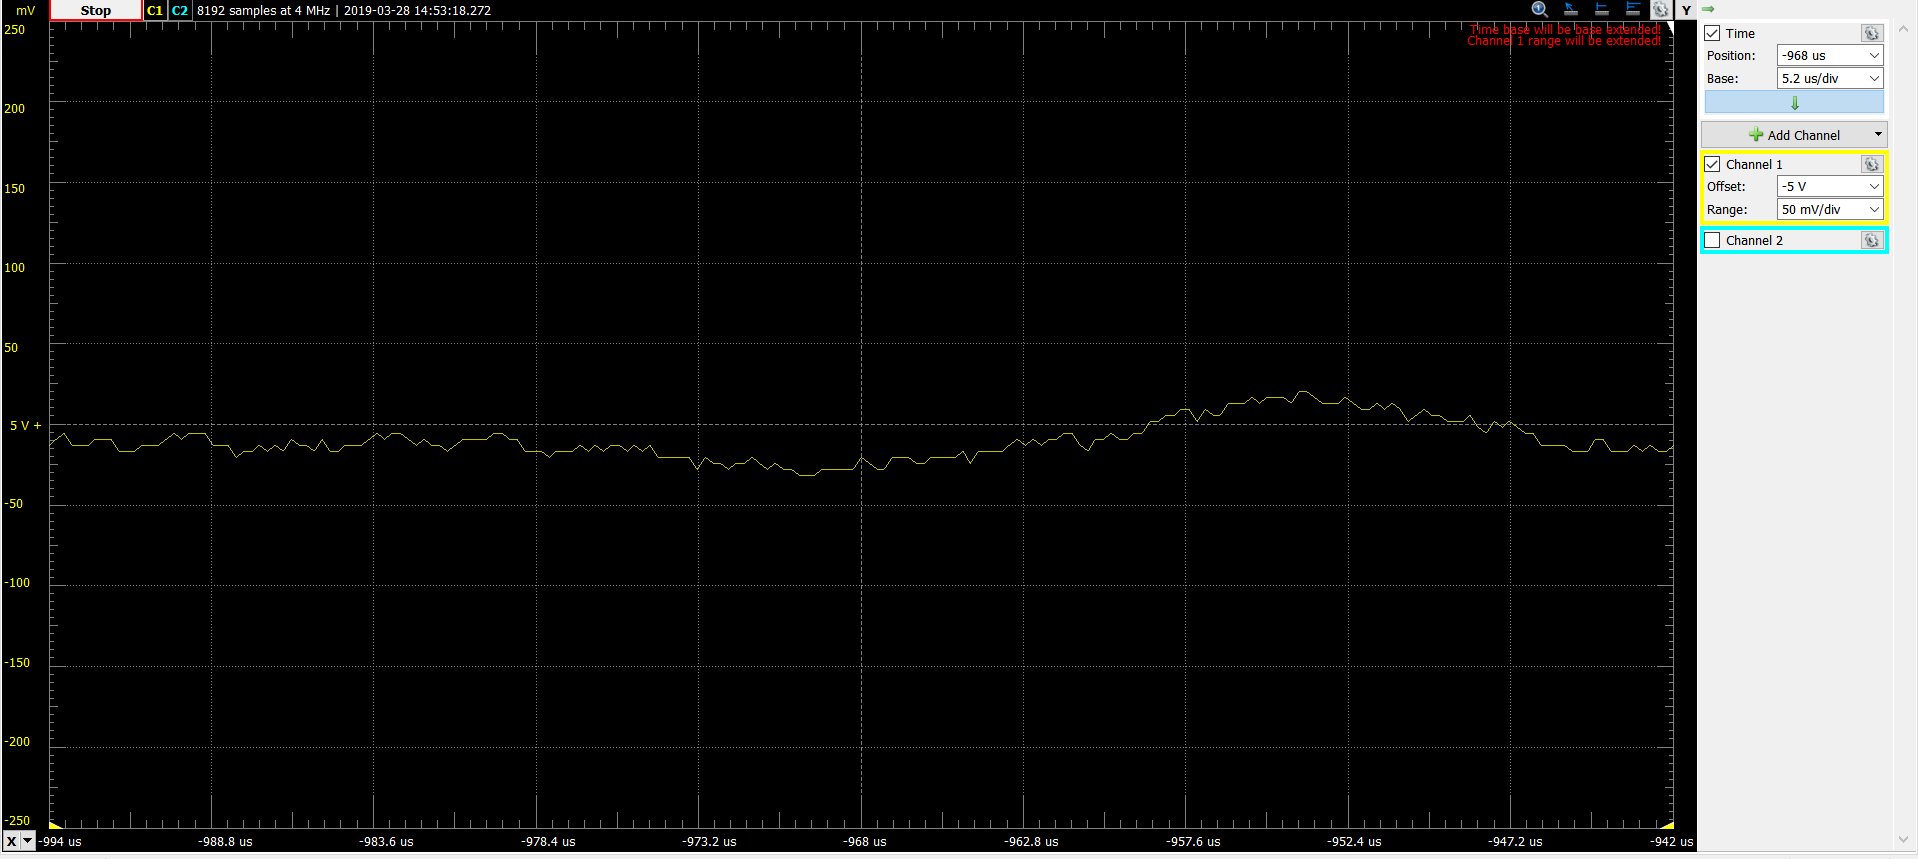
\includegraphics[width=0.5\textwidth]{./figurer/j10.png}
  \caption{Test af BUCK-konverter}
  \label{fig:j10}
\end{figure}

Som det ses, leveres en spænding omkring de 5 V. Denne spænding er acceptabel, om end vi ser en lille smule ripple. Denne kan skyldes den måde BUCK-konverteren virker på. Filteret der sidder efter konverteren, kan afvige en smule i praksis fra de teoretiske værdier. Det er dog stadig vigtigt at understrege, at dette output er acceptabelt. Strømmen måles til 1,3 A med loadmodstand.

Efter påvirkning af varme ændrede outputtet sig imidlertid ret dramatisk. Dette kan skyldes, at både dioden og TPS5410 er påvirkelige af varme, ligesom den induktive reaktans påvirkes i spolen. Her ses outputtet efter varmepåvirkningen har stået på i 30 sekunder. 

\begin{figure}[h]
  \centering
  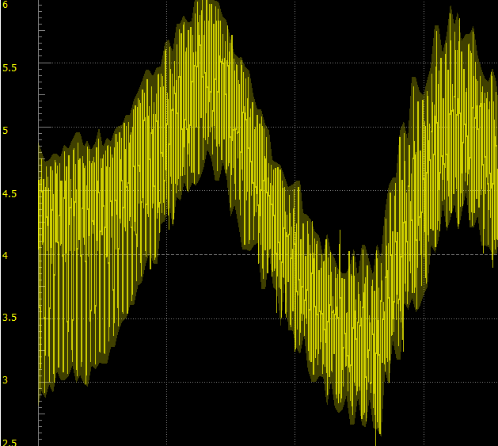
\includegraphics[width=0.5\textwidth]{./figurer/j11.png}
  \caption{Ændring af output}
  \label{fig:j11}
\end{figure}


Som det ses i figur \ref{fig:j11}, ændrer outputtet sig væsentligt! 

For at være sikker på, at komponenterne ikke var brændt af ved påvirkningen fra lighteren, køres en test cirka 15 minutter efter, hvor outputtet igen var standardiseret. 

For at kunne vælge endeligt imellem spændingsregulatorerne, opsættes følgende pointsystem
\begin{itemize}
\item Driftssikker, også ved påvirkning af varme - 2 P
\item Skal være den billigste, brugbare løsning - 2 P
\item Minimal ripple på output - 1 P
\item Minimal størrelse og vægt - 1 P
\end{itemize}

Pointfordelingen er som følger herunder, hvilket giver en klar sejr til LM317-systemet. Dette bygges på PCB og testes.
\begin{table}[h]
  \centering
% BEGIN RECEIVE ORGTBL jtab
\begin{tabular}{lrr}
\textbf{Kriterie} & \textbf{TPS5410} & \textbf{LM317-T} \\
\hline
Varmepåvirkning & 0 & 2 \\
Billigste løsning & 0 & 2 \\
Minimal ripple & 0 & 1 \\
Minimal størrelse & 1 & 0 \\
\hline
\textbf{Ialt} & \textbf{1} & \textbf{5} \\
\end{tabular}
% END RECEIVE ORGTBL jtab
  \caption{Point tabel}
  \label{tab:pointj}
\end{table}
\begin{comment}
#+ORGTBL: SEND jtab orgtbl-to-latex :splice nil :skip 0
| Kriterie          | TPS5410 | LM317-T |
|-------------------+---------+---------|
| Varmepåvirkning   |       0 |       2 |
| Billigste løsning |       0 |       2 |
| Minimal ripple    |       0 |       1 |
| Minimal størrelse |       1 |       0 |
|-------------------+---------+---------|
| Ialt              |       1 |       5 |
|-------------------+---------+---------|
\end{comment}

\subsection{Endelig test}
\label{sec:endelig-test}

Spændingsregulatoren blev meget enkelt testet ved at tilslutte en strømforsyning som input og tilslutte et voltmeter, for at måle udgangsspændingen. Opstillingen kan ses i figur \ref{fig:j12}. Som det fremgår af ovenstående billede, regulerer spændingsregulatoren fra 22 V til 5,3 V. Output spændingen er altså en smule højere end tilsigtet, men ikke mere end det accepteres. Da setuppet blev bygget på breadboard var outputspændingen på 5,1 V. Forskellen ligger i, at der er en større intern modstand på breadboardet end på PCB-printet, hvilket der ikke er blevet taget højde for. 

Efter spændingsregulatoren blev bygget på PCB burde vi have testet strømmen. Dette er en forglemmelse, og det må antages, at der stadig kan trækkes den fornødne strøm. 

\begin{figure}[h]
  \centering
  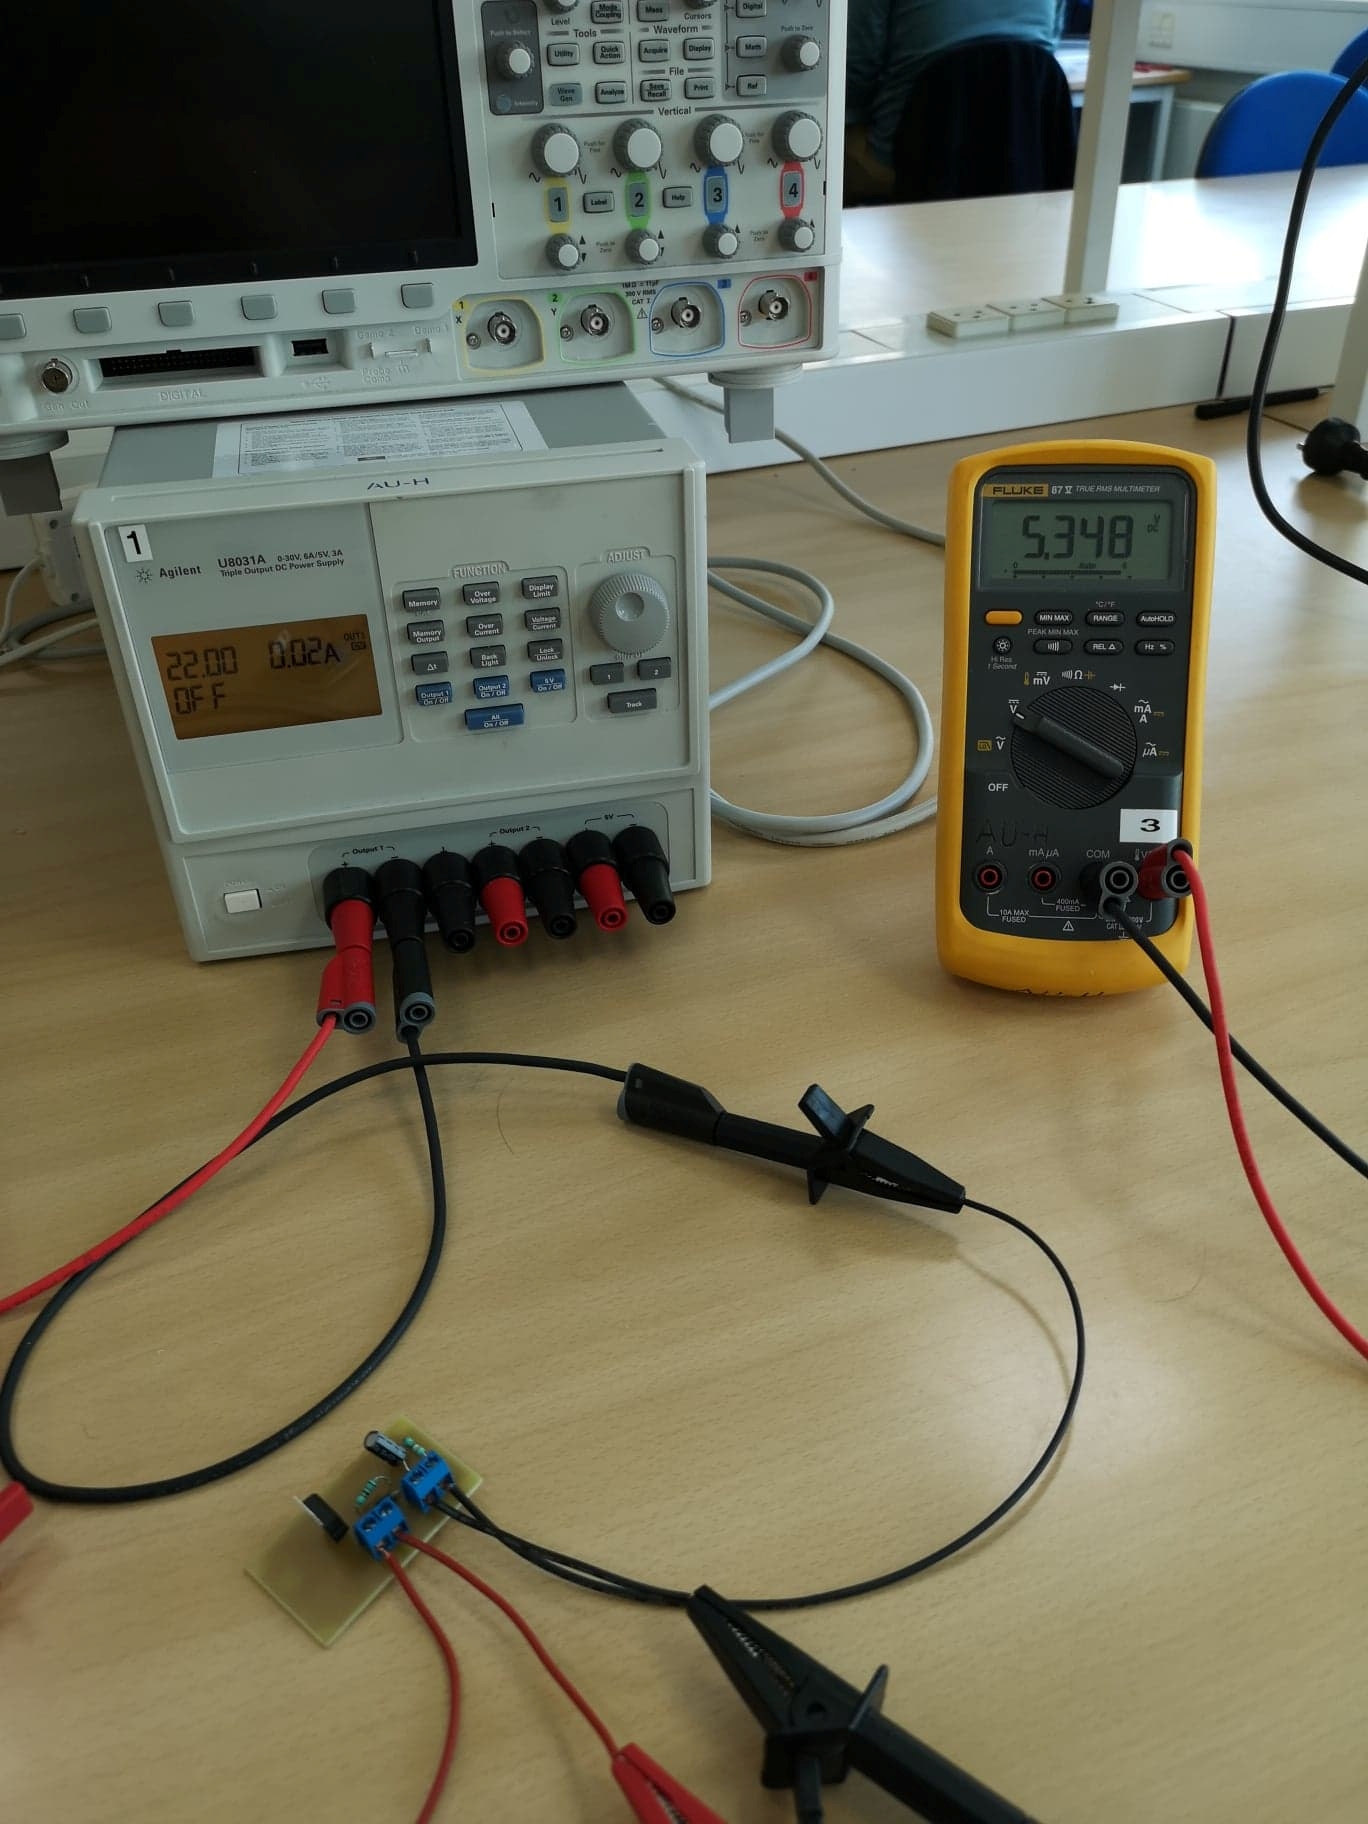
\includegraphics[width=0.4\textwidth]{./figurer/j12.png}
  \caption{Endelig test}
  \label{fig:j12}
\end{figure}

\clearpage
\section{Motorstyring}
\label{sec:motorstyring-1}

\subsection{Servo motor og ESC driver (Søren)}
\label{sec:servo-motor-og}

Servomotoren skal bruge et signal på 50 Hz for at fungere. Dette opnås ved at justere PWM mellem 1 ms til 2 ms aktiv høj, hvilket fremgår fra databladet på servomotoren (SG90 micro servo). Dette tillader at justere positionen på servomotoren fra 0 – 90 $^\circ$.

Dette signal bruges også til at justere hastigheden på BLDC-motor, via ESC'en. 1 ms blev brugt til stop af BLDC-motor og 1,3 ms, til at kunne starte motoren. 1,3 ms blev fundet via brug af et scope med et wavegen, hvor vi kom frem til at, at ved denne værdi, havde motoren nemt ved at starte. Følgende krav blev opsat, for at kunne verificere at det virkede efter hensigten

\begin{itemize}
\item 50 Hz signal, 20 ms periode (Krav nr. 2.1.3.8.1)
\item Skal kunne justere puls mellem 1 – 2 ms. (Krav nr. 2.1.3.8.2)
\end{itemize}

Ved at opsætte analog Discovery til på pin PTD3, se figur \ref{fig:mots4}, vises at init funktion (se figur \ref{fig:kodes1}) virker efter hensigten, med 50 Hz og 1 ms puls. Og hermed lever op til følgende krav 2.1.3.8.1 og 2.1.3.8.2, der er beskrevet tidligere.

\begin{figure}[h]
  \centering
  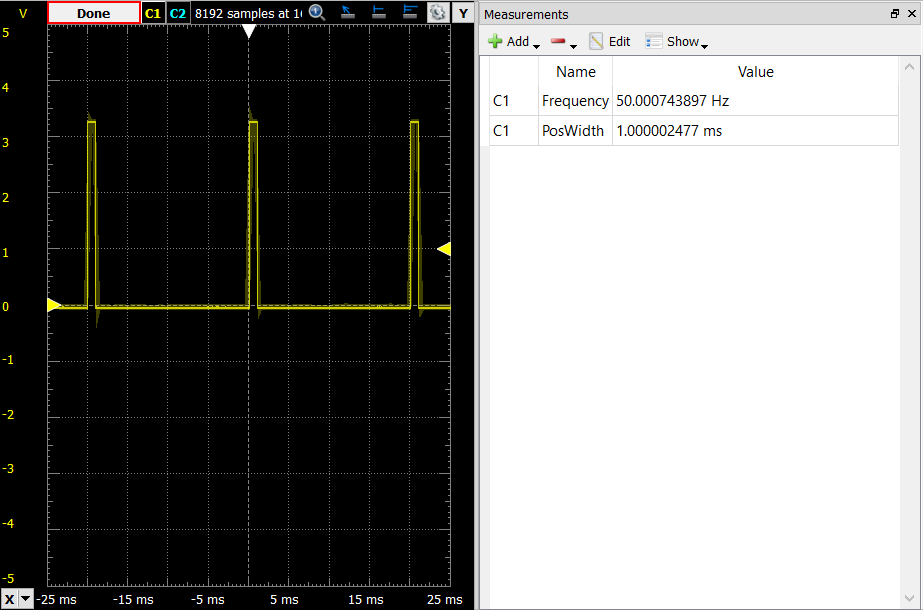
\includegraphics[width=0.8\textwidth]{./figurer/mots4.png}
  \caption{Test af init-funktion}
  \label{fig:mots4}
\end{figure}
\clearpage
\begin{figure}[h]
  \centering
  \lstinputlisting[language=c,firstline=39,lastline=101,basicstyle=\scriptsize\ttfamily]{./kode/servo-driver.cpp}  
  \caption{Opsætning af servo og ESC driver}
  \label{fig:kodes1}
\end{figure}
\clearpage

Herefter blev en funktion til at styre vores servomotor implementeret, se figur \ref{fig:kodes2}. Den tager et argument, som er en procentsats af hvor meget den skal dreje, i forhold til om den skal give fuld gas (100\%) eller køre i tomgang (0\%). Ved montering af servomotor (se evt. figur \ref{fig:mots5}), viste 1,4 ms signal til servomotoren sig at være fuldgas, hvilket blev tilpasset i koden. Såmax værdien der kunne sendes ud er 1,4 ms.

% \begin{figure}[!htb]
%     \centering
%     \begin{minipage}{.5\textwidth}
%         \centering
%   \lstinputlisting[language=c,firstline=102,lastline=107,basicstyle=\scriptsize\ttfamily]{./kode/servo-driver.cpp}
%   \label{fig:kodes2}
%     \end{minipage}%
%     \begin{minipage}{0.5\textwidth}
%         \centering
%         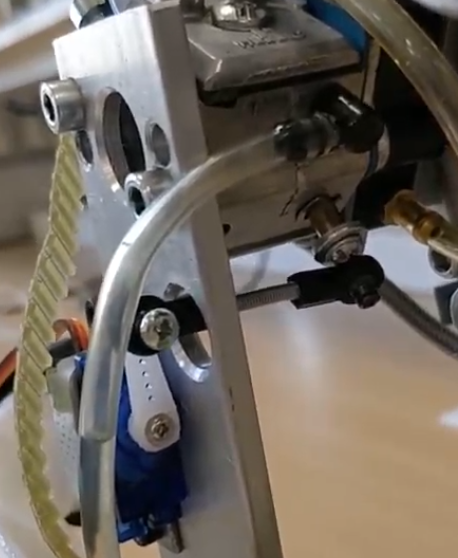
\includegraphics[width=0.5\linewidth]{./figurer/mots5.png}
%         \label{fig:mots5}
%     \end{minipage}
%     \caption{Kode til at styre gasspjældet}
%   \end{figure}

\begin{figure}[h]
  \centering
  \lstinputlisting[language=c,firstline=102,lastline=107,basicstyle=\scriptsize\ttfamily]{./kode/servo-driver.cpp}
  \caption{Servomotor monteret på gasspjæld}
  \label{fig:kodes2}
\end{figure}

  
\begin{figure}[h]
  \centering
  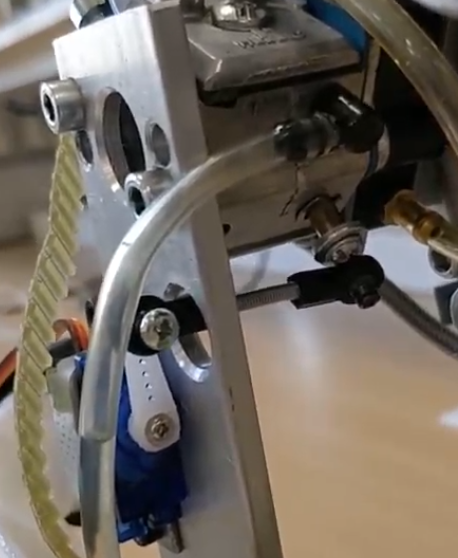
\includegraphics[width=0.5\textwidth]{./figurer/mots5.png}
  \caption{Servomotor monteret på gasspjæld}
  \label{fig:mots5}
\end{figure}

  
\subsection{Start af motoren}
\label{sec:start-af-motoren}

Driveren der bruges til at styre servomotoren var den samme, som skulle bruges for at kunne starte BLDC-motor, da den fungere som el-starter til motoren. Derfor blev der implementeret en pin ekstra, i driveren, der er vist i koden se figur \ref{fig:kodes3}. Herefter blev der lavet en start funktion, der skulle bruges til at starte motoren.

Flow for opstart af motor, ved funktionen \lstinline{start()}:

\begin{enumerate}
\item Startknap initialiseres.
\item Afventer at brugeren trykker på knappen.
\item En timer opsættes, som tæller vores ’i’ værdi op, når der er gået 500 ms.
\item Så prøver motoren at starte benzinmotoren, og det vil den gøre så længe start knappen er trykket ned (dog i maks. 15 sek).
\item Efter 15 sek vil opstartsprocessen afbrydes.
\end{enumerate}

\begin{figure}[h]
  \centering
  \lstinputlisting[language=c,firstline=132,lastline=154,basicstyle=\scriptsize\ttfamily]{./kode/servo-driver.cpp}
  \caption{Kode til \lstinline{start()}}
  \label{fig:kodes3}
\end{figure}

\begin{figure}[h]
  \centering
  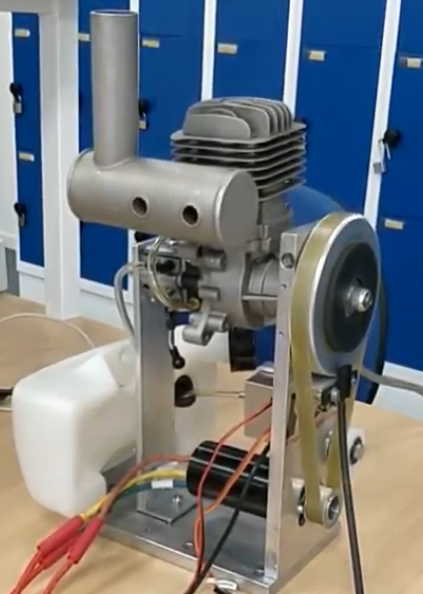
\includegraphics[width=0.3\textwidth]{./figurer/mots6.png}
  \caption{BLDC-motor forbundet til motoren med en tandrem}
  \label{fig:mots6}
\end{figure}
\clearpage
\subsection{RPM-detektering}
\label{sec:rpm-detektering}

Der er blevet udviklet kode til at aflæse rpm, se figur \ref{fig:kodes3}, som bruges til i forbindelse med PID-regulering. Der er taget udgangspunkt i at aflæse et tacho signal som kommer fra tændspolen. Dette signal lave en høj spænding ved hver omdrejning og går lav igen. For at afkode dette signal, bruges der input capture, der er implementeret i TPM periferenheden på KL25. Funktionen input capture, fungere ved at tælle op til hver ’rising edge’ og gemmer denne værdi. Når værdien og frekvensen der tælles op med er kendt, kan dette omregnes til RPM ved formlen:
\begin{equation}
  \label{eq:4}
 60 \mathrm{sek} \cdot \frac{\mathrm{frekvens}}{\mathrm{input\ capture\ værdien}}=\mathrm{RPM} 
\end{equation}

Selve koden er vist i figur \ref{fig:kodes3}. Der bruges interrupts til at opfange overflows og rising edge hvorved værdien gemmes i CNV-registeret. TPM1 modulet initialiseres og frekvensen der bruges til at tælle op med, bliver nedskaleret, til 375 kHz. Dvs. imellem hvert overflow går der 5,75 Hz, hvilket passer med måleområdet (17 - 167 Hz) som der arbejdes indenfor.

\begin{figure}[h]
  \centering
  \lstinputlisting[language=c,firstline=39,lastline=58,basicstyle=\scriptsize\ttfamily]{./kode/rpm-detect.cpp}  
  \caption{Kode til RPM-detektering}
  \label{fig:kodes3}
\end{figure}


\subsection{Stepinput og overføringsfunktion (Simon)}
\label{sec:tests}

PID-koefficienterne skal defineres udfra en overføringsfunktion for vores system som skal reguleres. For at udlede overføringsfunktionen blev et forsøg med optagelse af steprespons udarbejdet.

% Et testprogram kan køres via microcontroller som foretager PID-reguleringen og optage motorens omdrejninger ved forskellige skift mellem hastigheder. Disse gentages for forskellige værdier af $K_p$ og $K_i$.

Som udgangspunkt vil strømmen fra dronecopteren til batteri være variende.%skal forholdet mellem dronens hastighed og %skulle det interessante for dronecopteren være at % I en teststand vil formålet være at test forskellige værdier af koefficienterne og i forskellige kombinationer. Målet med PID-reguleringen er at
%strømmen fra batteri til dronens propelmotorer være konstant.

Tilgengæld skal spjældet til forbrændingsmotoren konstant reguleres. Derfor vil en teststand som udgangspunkt have følgende:
\begin{itemize}
\item input: strøm fra batteri til drone
\item output: regulering af spjæld via servomotor
\end{itemize}

Her vil $e(t)$ være et mål for forskellen mellem den ønskede strømstyrke og den faktiske.

Det var ikke muligt at måle strømmen fra batteri til drone. For at lave en teststand som kan tjene som demonstration af PID-regulering samt som skabelon for senere tests fremstilles istedet en teststand som skal justere spjældet i forhold til motorens omdrejninger. Dvs:

\begin{itemize}
\item input: motorens omdrejninger
\item output: regulering af spjæld via servomotor
\end{itemize}

I dette tilfælde vil $e(t)$ være et mål for forskellen mellem det ønskede omdrejningstal og det faktiske.

For at få en grov ide om niveauet af koefficienterne kan en simulink simulation være gunstig. I denne skal gøres en række antagelser af forholdet mellem spjældvinkel og omdrejningstallet. Når koefficienterne er tunet i simulink kan der laves en test.

% I testen skal der laves forskellige trinsvise ændringer af omdrejningstallet. Fjare\autocite{pid1} har beskrevet hvordan 4 forskellige trinmønstre (se figur\ref{fig:paths}) blev brugt til at justere en PID-algoritme som blev brugt til en forbrændingsenhed i en ubemandet flyvende enhed.

% \begin{figure}[h]
%   \centering
%   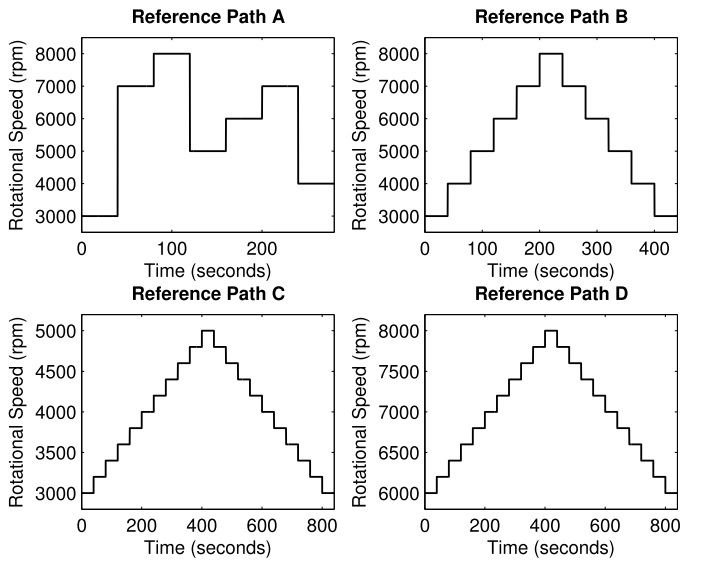
\includegraphics[width=0.7\textwidth]{refpaths.JPG}
%   \caption{Trinmønstre}
%   \label{fig:paths}
% \end{figure}

% På trods af at forbrændingsenheden altså ikke opladet batteri virker det relevant at tage udgangspunkt i lignende trinmønste til PID-kontrol af motoromdrejninger.

% KL25 vil tjene både som microcontroller og datalogger.

\subsubsection{Steprespons}
\label{sec:steprespons}

%For at simplificere PID-reguleringen forsøges forst med regulering af spjæld i forhold til motorens omdrejninger.
Der vil tages udgangspunkt i måling af et steprespons på motorens omdrejninger. Til målinger af omdrejninger anvendtes et oscilloskop som optog data fra Hall-sensoren. Optagelsen blev tricket fra KL25Z.% foreslås at bruge Pocketbeagle som vil kunne foretage måling af omdrejninger via Hall-sensor og lagre data i en fil som kan eksporteres til analyse i Matlab.

Data fra oscilloskopet bestod i 50000 målinger som bestod af Hall-sensorens spænding, spændingen fra servomotoren, der styrer spjældet, samt et tidsmål. Nedenfor ses et udsnit af de 50000 målinger:

\begin{table}[h]
  \centering
% BEGIN RECEIVE ORGTBL tabel4
\begin{tabular}{r|r|r}
\hline
\textbf{second} & \textbf{Volt} & \textbf{Volt1} \\
\hline
-1 & 0.215206000000000 & 4.98492460000000 \\
-0.999900000000000 & 0.215206000000000 & 4.90452260000000 \\
-0.999800000000000 & 0.134804000000000 & 4.90452260000000 \\
-0.999700000000000 & 0.215206000000000 & 4.98492460000000 \\
-0.999600000000000 & 0.215206000000000 & 4.90452260000000 \\
-0.999500000000000 & 0.215206000000000 & 4.90452260000000 \\
-0.999400000000000 & 0.215206000000000 & 4.90452260000000 \\
-0.999300000000000 & 0.215206000000000 & 4.82412060000000 \\
-0.999200000000000 & 0.215206000000000 & 4.90452260000000 \\
\hline
\end{tabular}
% END RECEIVE ORGTBL tabel4
  \caption{}
  \label{tab:komp3}
\end{table}
\begin{comment}
#+ORGTBL: SEND tabel4 orgtbl-to-latex :splice nil :skip 0
|--------------------+-------------------+------------------|
|             second |              Volt |            Volt1 |
|--------------------+-------------------+------------------|
|                 -1 | 0.215206000000000 | 4.98492460000000 |
| -0.999900000000000 | 0.215206000000000 | 4.90452260000000 |
| -0.999800000000000 | 0.134804000000000 | 4.90452260000000 |
| -0.999700000000000 | 0.215206000000000 | 4.98492460000000 |
| -0.999600000000000 | 0.215206000000000 | 4.90452260000000 |
| -0.999500000000000 | 0.215206000000000 | 4.90452260000000 |
| -0.999400000000000 | 0.215206000000000 | 4.90452260000000 |
| -0.999300000000000 | 0.215206000000000 | 4.82412060000000 |
| -0.999200000000000 | 0.215206000000000 | 4.90452260000000 |
|--------------------+-------------------+------------------|
\end{comment}

Spændingen fra Hall-sensoren, Volt1, anvendes.
Når data plottes for et kort tidsrum ses støj omkring 5 volt

\begin{figure}[h]
  \centering
  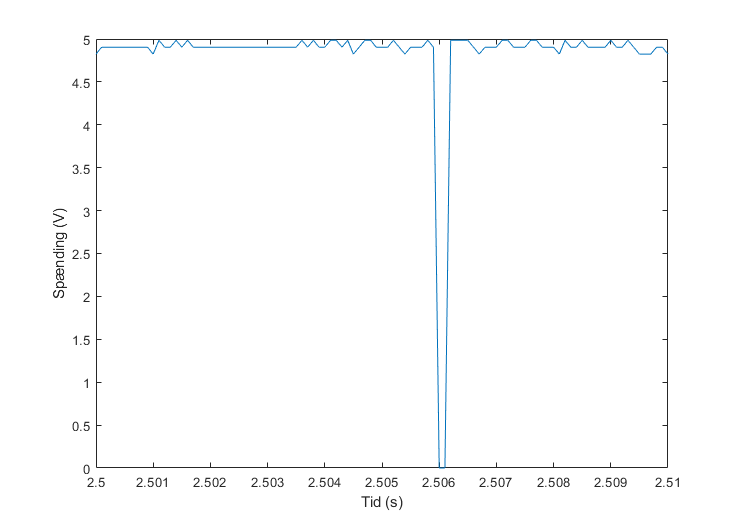
\includegraphics[width=0.6\textwidth]{./figurer/mo1.png}
  \caption{}
  \label{fig:mo1}
\end{figure}
\clearpage
Data processeres nu med følgende Matlab-script:
\begin{lstlisting}[language=Matlab]
close all
data = stepdata5;
t = data.second;
v = data.Volt1;
border1 = 4.5;
border2 = 0.1;
v2 = data.Volt;
b = 0;
stop = 0;
tp = [];
tpt = [];
vpt0 = [];
i = 1;
nyv = [];
while (i <= length(t))
    if (v(i)>border1)
        vn = 5;
    else
        vn = 0;
    end
    nyv = [nyv vn];
    i = i + 1;
end
i = 1;


while (i < length(t))
    if ((nyv(i+1)>border1 & nyv(i)<border2) & b == 0)
        t1 = t(i+1);
        stop = 1;
        b = 1;
    end
    i = i + 1;
    vpt0 = [vpt0 0];
    while (stop ~= 2 & b == 1 & i < length(t))
        if (stop == 1)
            while (stop ~= 2 & i < length(t))
                if (nyv(i+1)>border1 & nyv(i)<border2)
                    t2 = t(i+1);
                    stop = 2;
                end
                i = i + 1;
                vpt0 = [vpt0 0];
            end
        end
        if (stop == 2)
            period = t2-t1;
            tpt = [tpt t2];
            vpt0(i) = nyv(i);
            tp = [tp period];
            t1 = t2;
            stop = 1;
        end
    end
end  
\end{lstlisting}

I scriptet fortolkes spænding over 4,5 V som 5 V. Markering af periodegrænser ved 5 Volt kan ses her (de røde prikker øverst):

\begin{figure}[h]
  \centering
  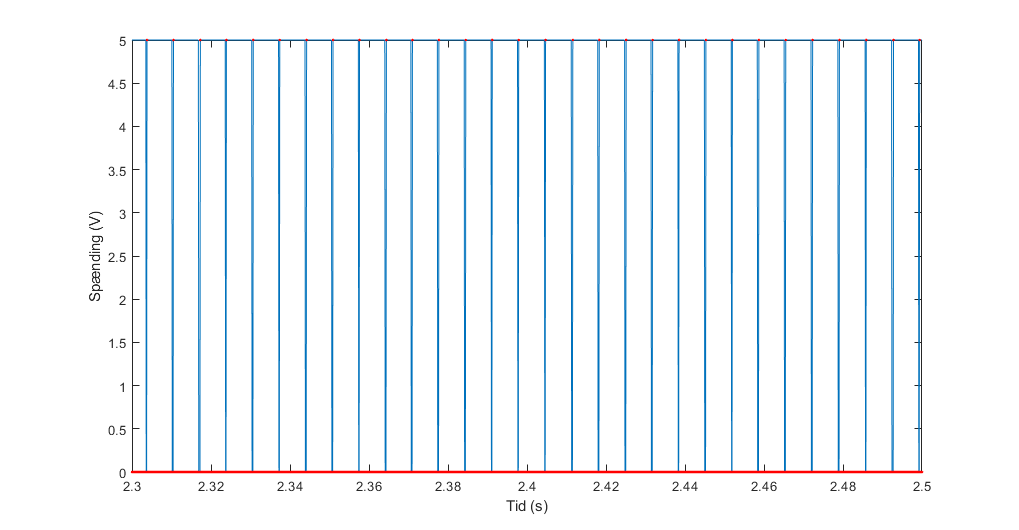
\includegraphics[width=0.6\textwidth]{./figurer/mo2.png}
  \caption{}
  \label{fig:mo2}
\end{figure}

Herudover udregnes tiden for hver omdrejningsperiode og gemmes i vektoren ”tp”.
Ved plot at tp givet ved rpm overfor tid fås:

\begin{figure}[h]
  \centering
  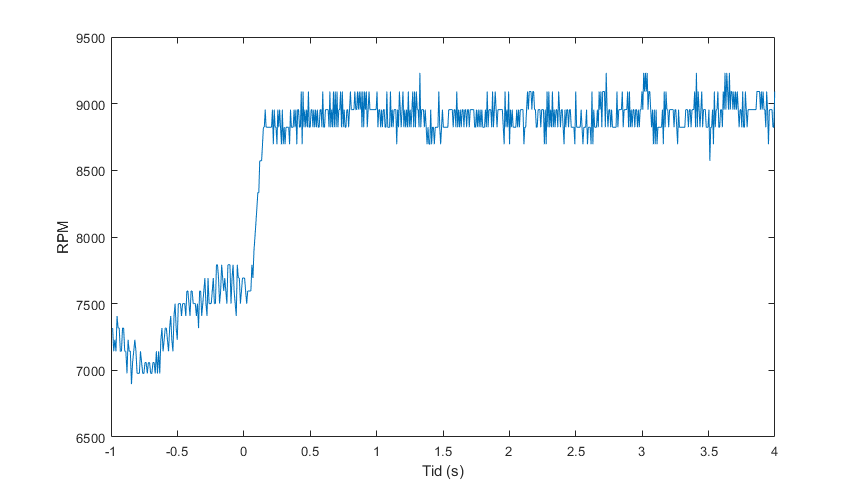
\includegraphics[width=0.6\textwidth]{./figurer/mo3.png}
  \caption{}
  \label{fig:mo3}
\end{figure}

\subsubsection{Overføringsfunktion}

\label{sec:overforingsfunktion}
Udfra stepresponset skal følgende identificeres:

\begin{itemize}
\item Rise time, $t_r$
\item Settling time, $t_s$
\item Overshoot, $M_p$
% \item Peak time, $t_p$
\end{itemize}

Scopet der har målt data gemmer også data op til stepresponset. Stepresponset ses ved tiden 0.
Ved at applicere et midlingsfilter på 200 fås et indtryk af et steady-state niveau ved 8900, med start fra 7600, dvs 1300. 

\begin{figure}[h]
  \centering
  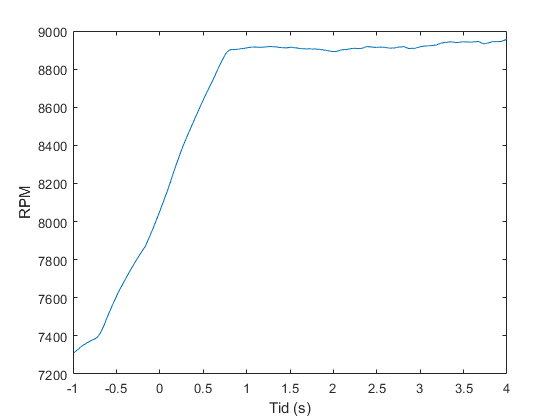
\includegraphics[width=0.5\textwidth]{./figurer/mo4.png}
  \caption{}
  \label{fig:mo4}
\end{figure}

Ved at applicere et midlingsfilter på 10 fås et indtryk af en 1. grads overføringsfunktion.

\begin{figure}[h]
  \centering
  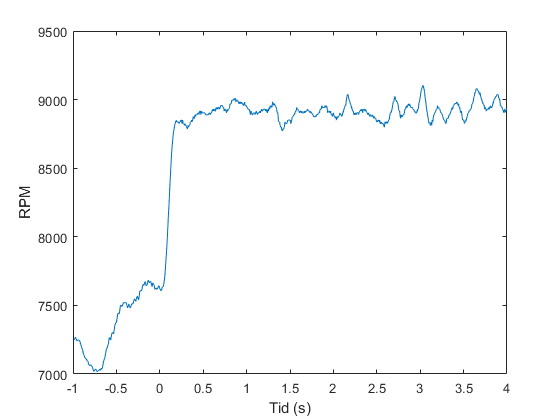
\includegraphics[width=0.5\textwidth]{./figurer/mo5.png}
  \caption{}
  \label{fig:mo5}
\end{figure}

Det måles at steady-state er opnået ved 0,19 sekunder. Dvs. $0.19 = 5\tau \Leftrightarrow \frac{0,19}{5}=\tau=0,04$.

Hermed kan overføringsfunktionen sættes som
\begin{equation}
  \label{eq:1}
G(s) = \frac{1300}{0,04s+1}  
\end{equation}

% I sidste timebox fandtes overføringsfunktionen
% \begin{equation}
%   \label{eq:1}
% G(s) = \frac{8900}{0,04s+1}  
% \end{equation}

I Simulink oprettes følgende:

\begin{figure}[h]
  \centering
  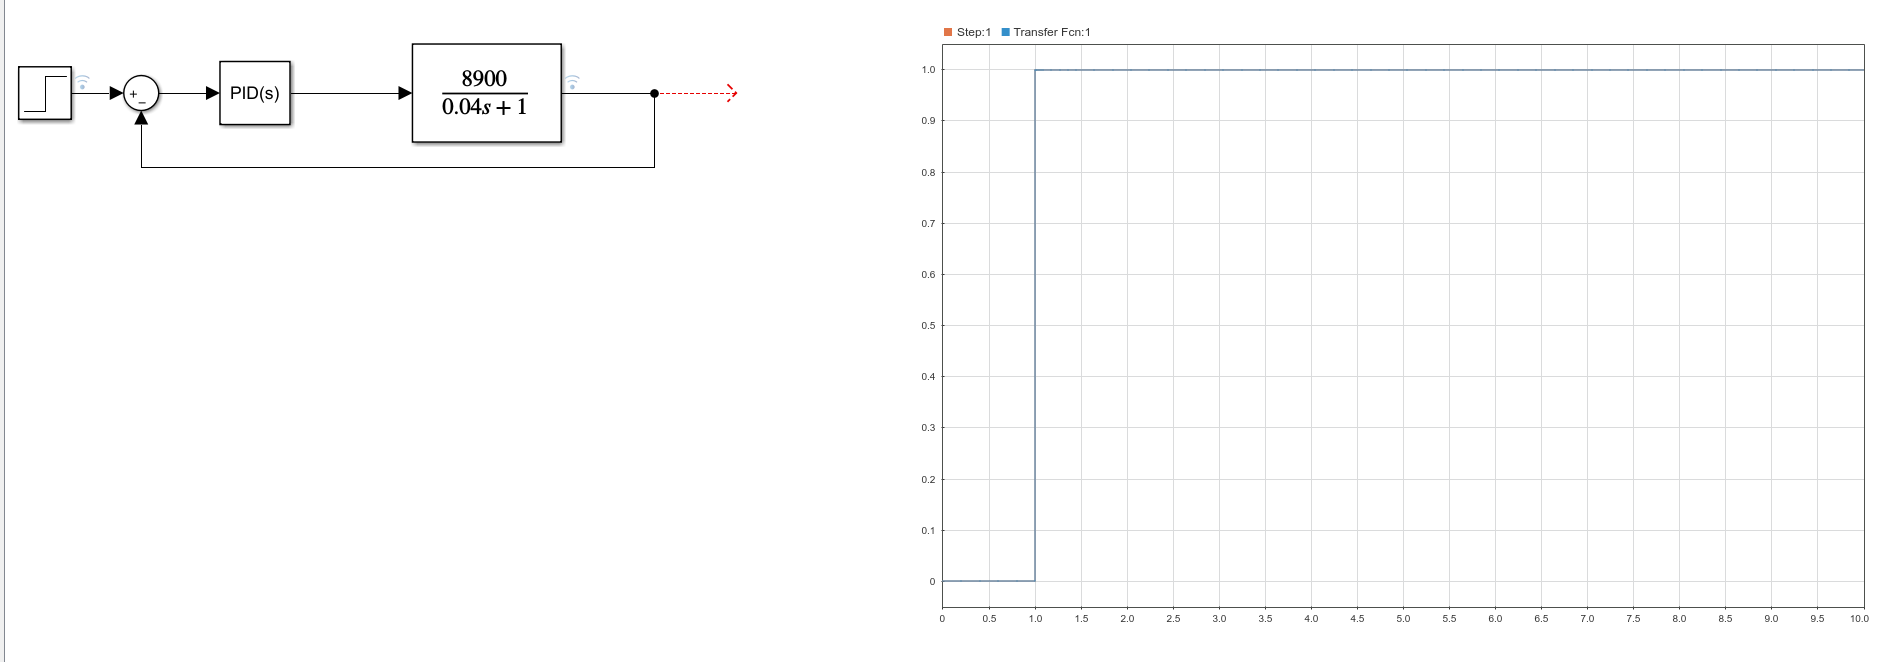
\includegraphics[width=0.6\textwidth]{./figurer/sbil1.png}
  \caption{Simulink - diagram}
  \label{fig:sbil1}
\end{figure}

Herefter laves autotuning i PID-modulet. Der findes koefficienter svarende til $P=0,0010$, $I=0,0514$, $D=-1,4946$ og følgende respons:

\begin{figure}[h]
  \centering
  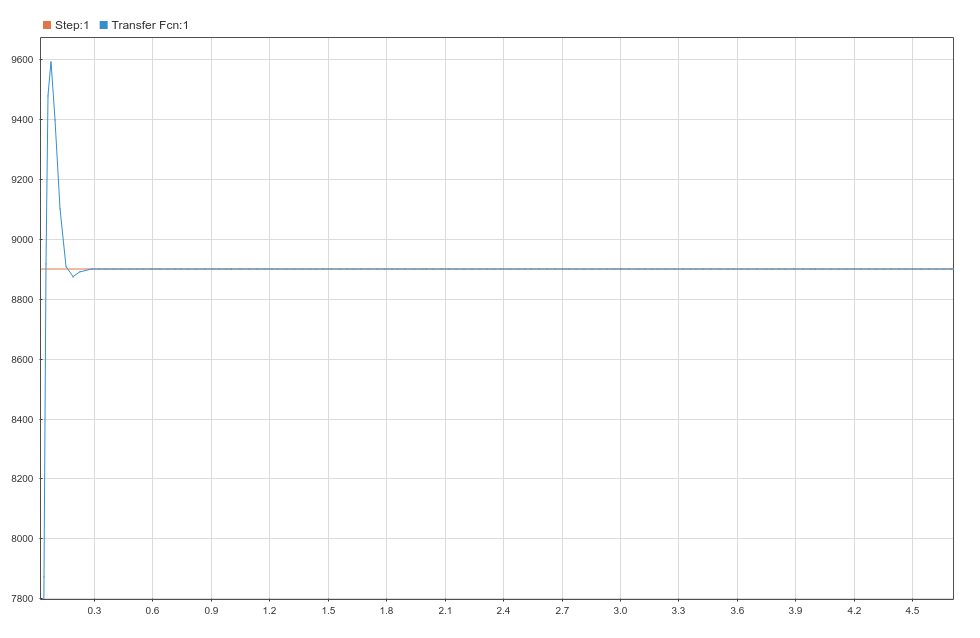
\includegraphics[width=0.6\textwidth]{./figurer/sbil2.png}
  \caption{Simulink - diagram 2}
  \label{fig:sbil1}
\end{figure}

\subsection{Software (Simon)}
\label{sec:software-1}

Der udarbejdes nu et udkast til PID-kontrol software som også benytter sig af software til kontrol af servomotor samt aflæsning af motorens omdrejninger (se afsnit \ref{sec:rpm-detektering}).

\begin{lstlisting}[language=C,basicstyle=\scriptsize\ttfamily]
#include <stdio.h>
#include "board.h"
#include "peripherals.h"
#include "pin_mux.h"
#include "clock_config.h"
#include "MKL25Z4.h"
#include "fsl_debug_console.h"
#include "rpm-detect.h"
#include "servo_driver.h"

// Filtrering
double alpha = 0.2;
double measuredSpeed = 0 ;

// Koefficienter
double kp = 0.001;
double ki = 0.0514;
double kd = -1.4946;
double K1;
double K2;
double K3;

// Vægtning af koefficienter
double setpointWeight = 0.2;
double lowpassSpeed;
double setpointSpeed;

// Diverse
double output;
double throttleopen = 1.0;
float throttlePos;

int rpmch;
int MAX_RPM = 9000;

// Initialiering
double lastSetpointSpeed = 0;
double lastMeasuredSpeed = 0;
double lastLowpassSpeed = 0;
double lastOutput = 0;
double lastLastMeasuredSpeed = 0;

void velPID (int setpointSpeed, int measuredSpeed) {
    lowpassSpeed = alpha * lastLowpassSpeed + (1-alpha ) * measuredSpeed;
    K1 = kp * setpointWeight * (setpointSpeed-lastSetpointSpeed) + kp * (lastMeasuredSpeed-lowpassSpeed);
    K2 = ki * (setpointSpeed-lowpassSpeed);
    K3 = kd * (2 * lastMeasuredSpeed-lowpassSpeed-lastLastMeasuredSpeed);
    output = lastOutput-K1-K2-K3;
    if (output < 0) {
      output = 0;
    }
    throttlePos = output/MAX_RPM;
    lastLowpassSpeed = lowpassSpeed;
    lastLastMeasuredSpeed = lastMeasuredSpeed;
    lastMeasuredSpeed = lowpassSpeed;
    lastSetpointSpeed = setpointSpeed;
    lastOutput = output;
    angle_throttle(throttlePos);
}

init_read_rpm()

int main(void) {
  /* Init board hardware. */
  BOARD_InitBootPins();
  BOARD_InitBootClocks();
  BOARD_InitBootPeripherals();
  /* Init FSL debug console. */
  BOARD_InitDebugConsole();
  rpmch = 7000;
  init_pwm();
  start();
  velPID(rpmch, measuredSpeed);
  return 0 ;
}

\end{lstlisting}


% Udfra disse mål kan der gives et bud på en overføringsfunktion. I matlab kan der via simulink og en overføringsfunktion findes PID-koefficienter og laves tuning. I slutningen af arbejdet undersøges om følgende kravene overholdes:
% \begin{itemize}
% \item Overshoot skal ikke være mere en 197 rpm.
% \item Justeringstiden må max være 8,8 sekunder.
% \item Ifm. et step respons skal 90 \% af målet være opnået i mindre end 3 sekunder.
% \end{itemize}

% Der er tidligere blevet lavet målinger ved steprespons af forbrændingsmotor. 

\clearpage
\chapter{Resultater}
\label{sec:resultater}

\section{Aktiv ensretter}
\label{sec:aktiv-ensretter}

Ud fra den nedskalerede funktionalitetstest af den aktive ensretter, hvor inputspænding vs. outputspænding plottes og spændingsfaldet beregnes i Matlab, kan det konkluderes, at kredsløbet indledningsvist levede op til kravet om ikke at have et spændingsfald på udgangen på mere end 0.7 volt i forhold til indgangen. 

Det viste sig dog, at kredsløbet begyndte at reagere uhensigtsmæssigt, når det blev belastet med en større load. Vi indledte fejlsøgning på kredsløbet og konstaterede, at spændingsniveauerne på MOSFET transistorernes gates varierede meget, hvorefter vi måtte stoppe udviklingen på grund af manglende tid.  

\section{Spændingsregulator}
\label{sec:spandingsregulator}





\section{Motorstyring}
\label{sec:motorstyring-2} 

Der blev lavet implementering af PID-koden. Resultatet var desværre at der ved øgning af mindskning af omdrejningstal blev lavet en stigning i omdrejningstal og omvendt.


% \bibliographystyle{unsrt}

\clearpage
% \appendix
% \addcontentsline{toc}{section}{Bilag}
% \vspace*{\fill}
% \begin{center}
% \Huge{  \textbf{BILAG}}
% \end{center}
% \vspace*{\fill}

% % \appendixpage
% % \addappheadtotoc

% \addcontentsline{toc}{section}{Timebox 1}
% \label{sec:timebox-1}
% 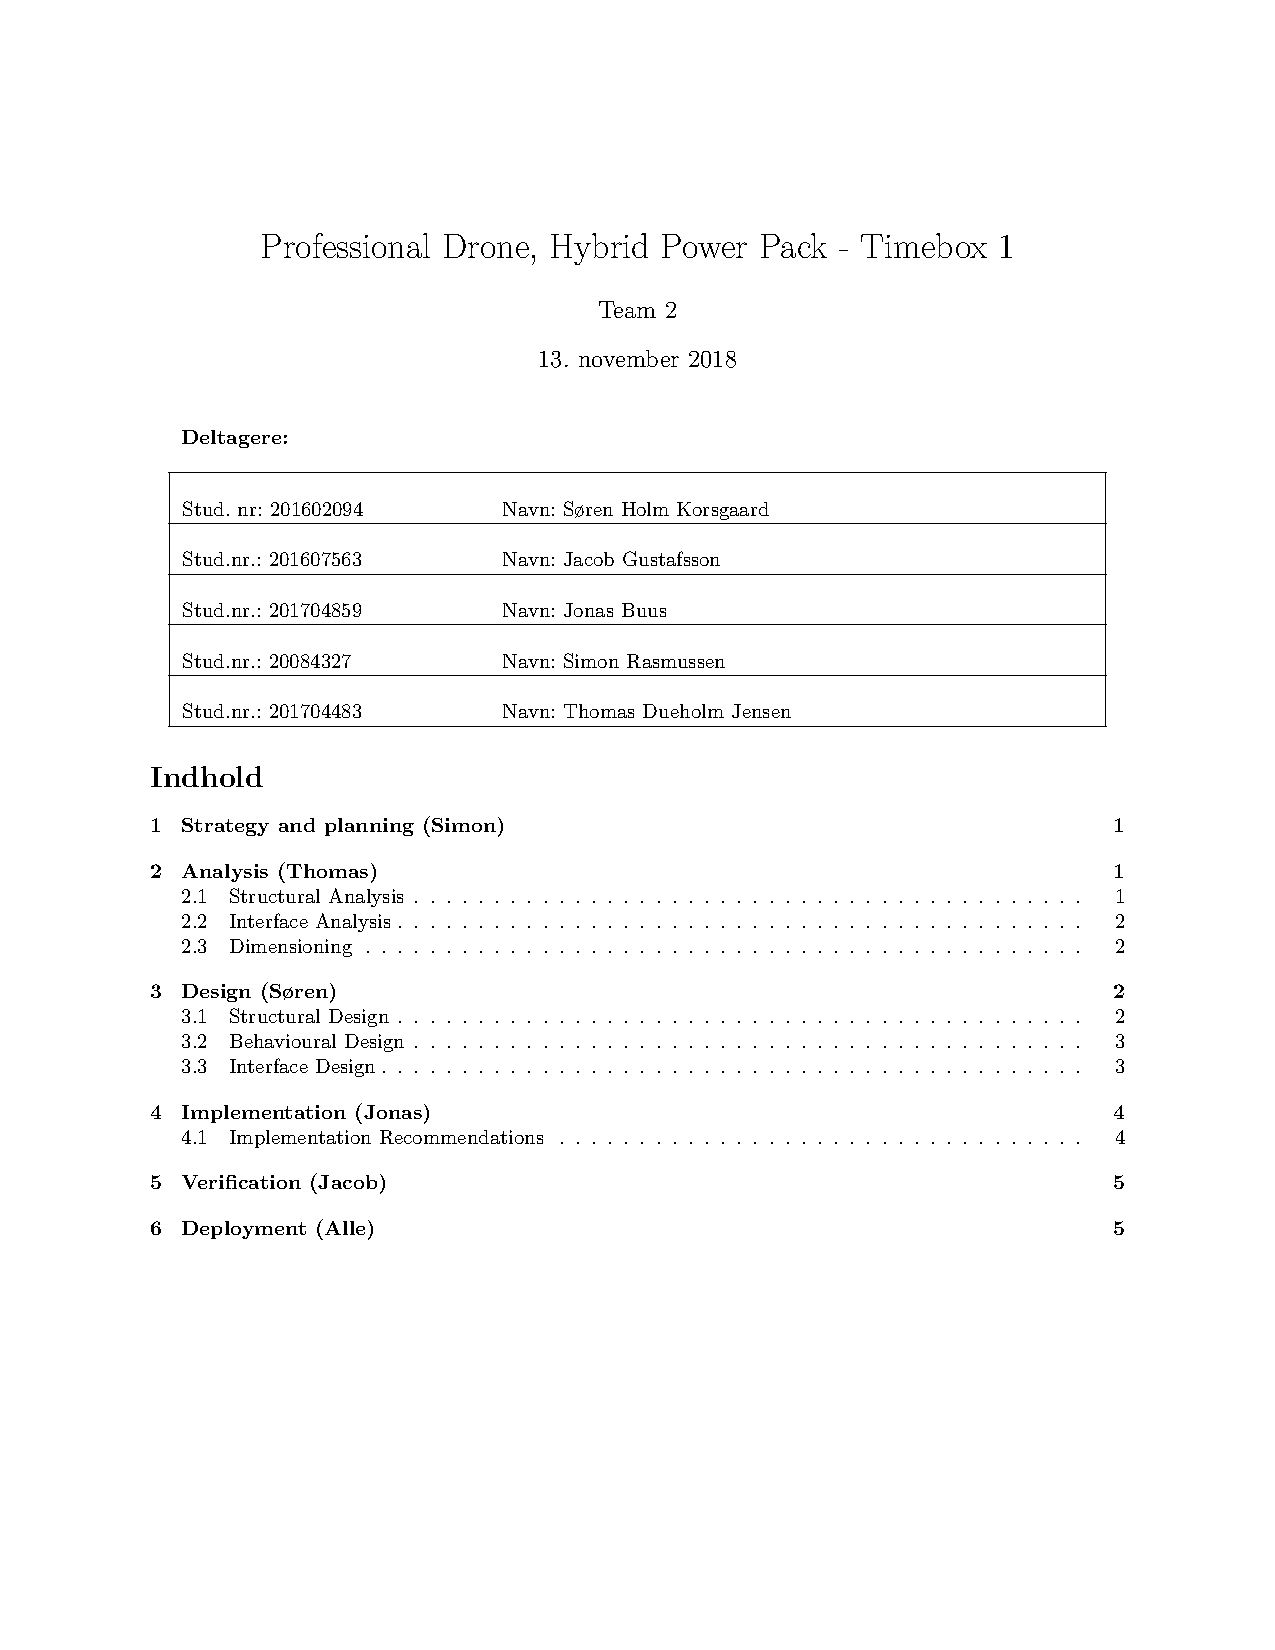
\includepdf[pages={-}]{timebox1-131118}
% \clearpage

% \addcontentsline{toc}{section}{Timebox 2}
% \label{sec:timebox-2}
% 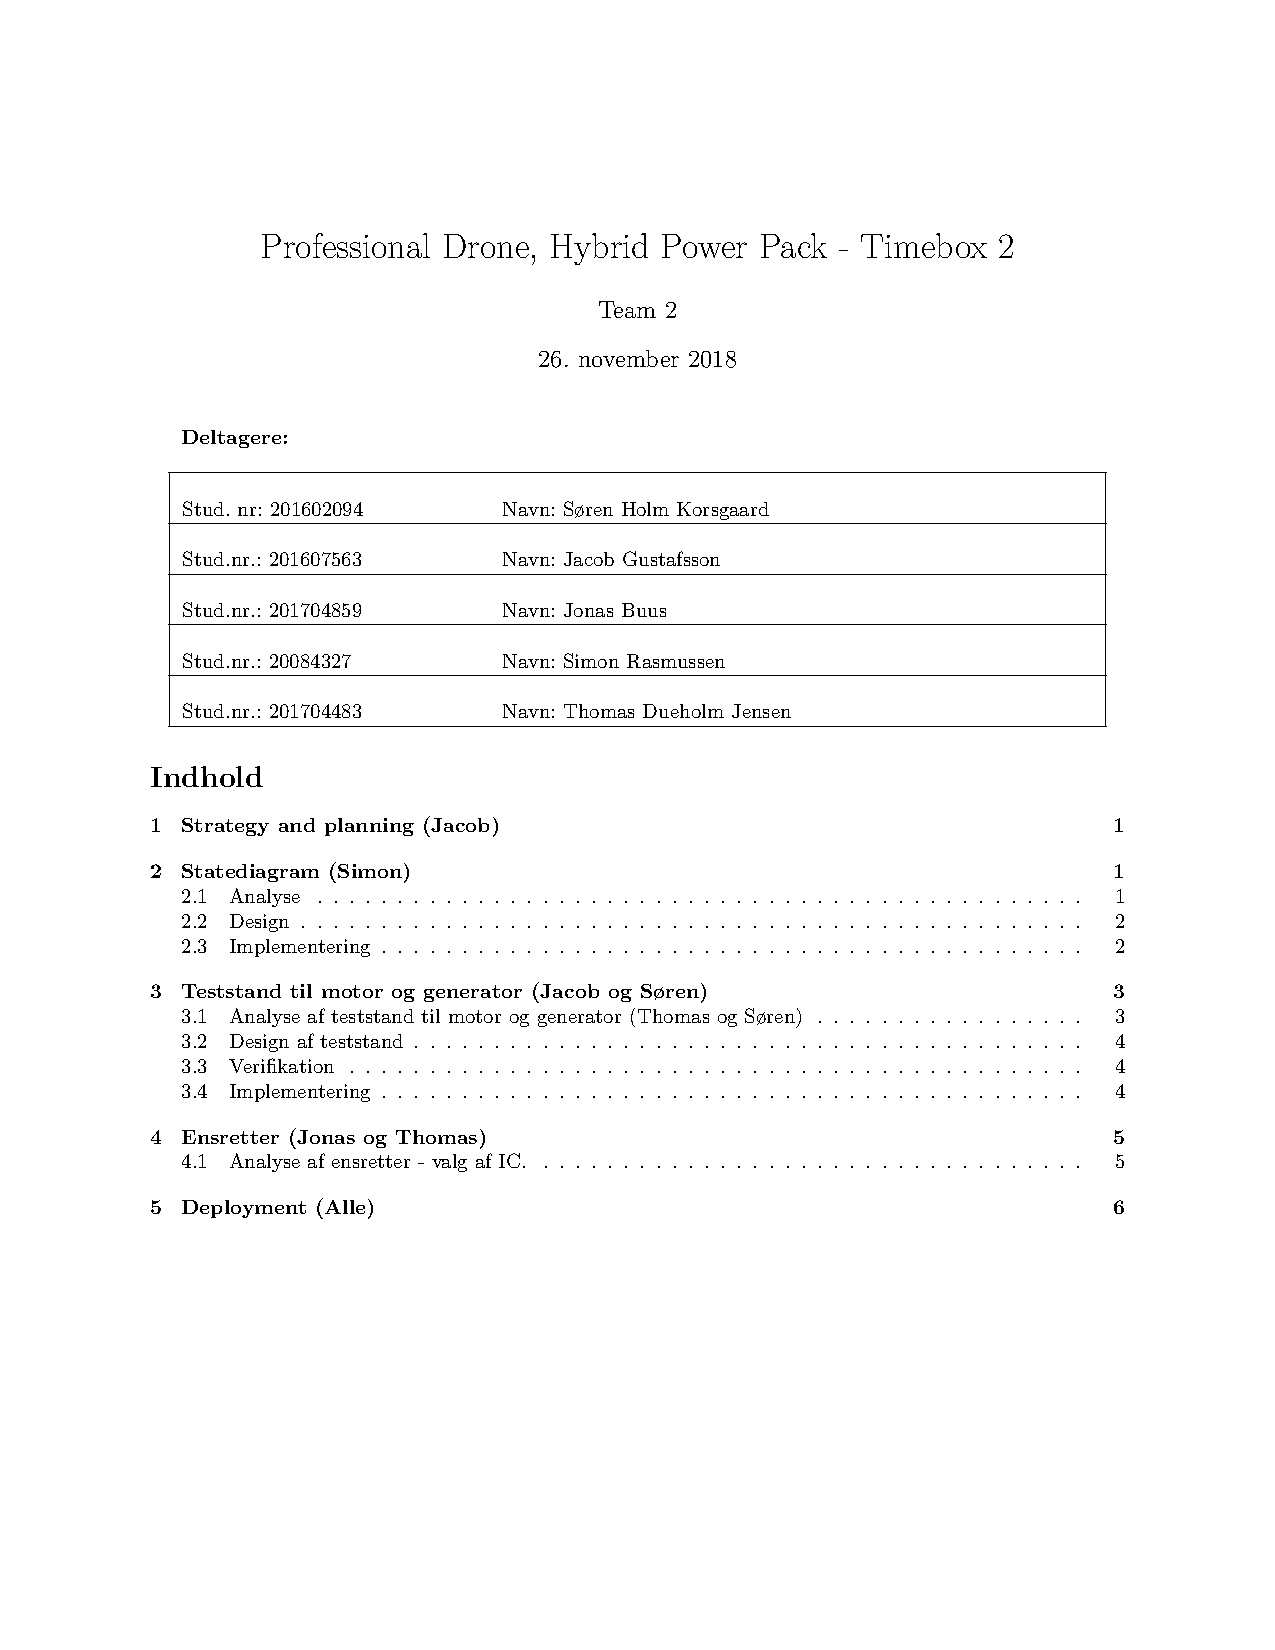
\includepdf[pages={-}]{timebox2-rettelse-fra-klaus(031218)}
% \clearpage

% \addcontentsline{toc}{section}{Timebox 3}
% \label{sec:timebox-3}
% 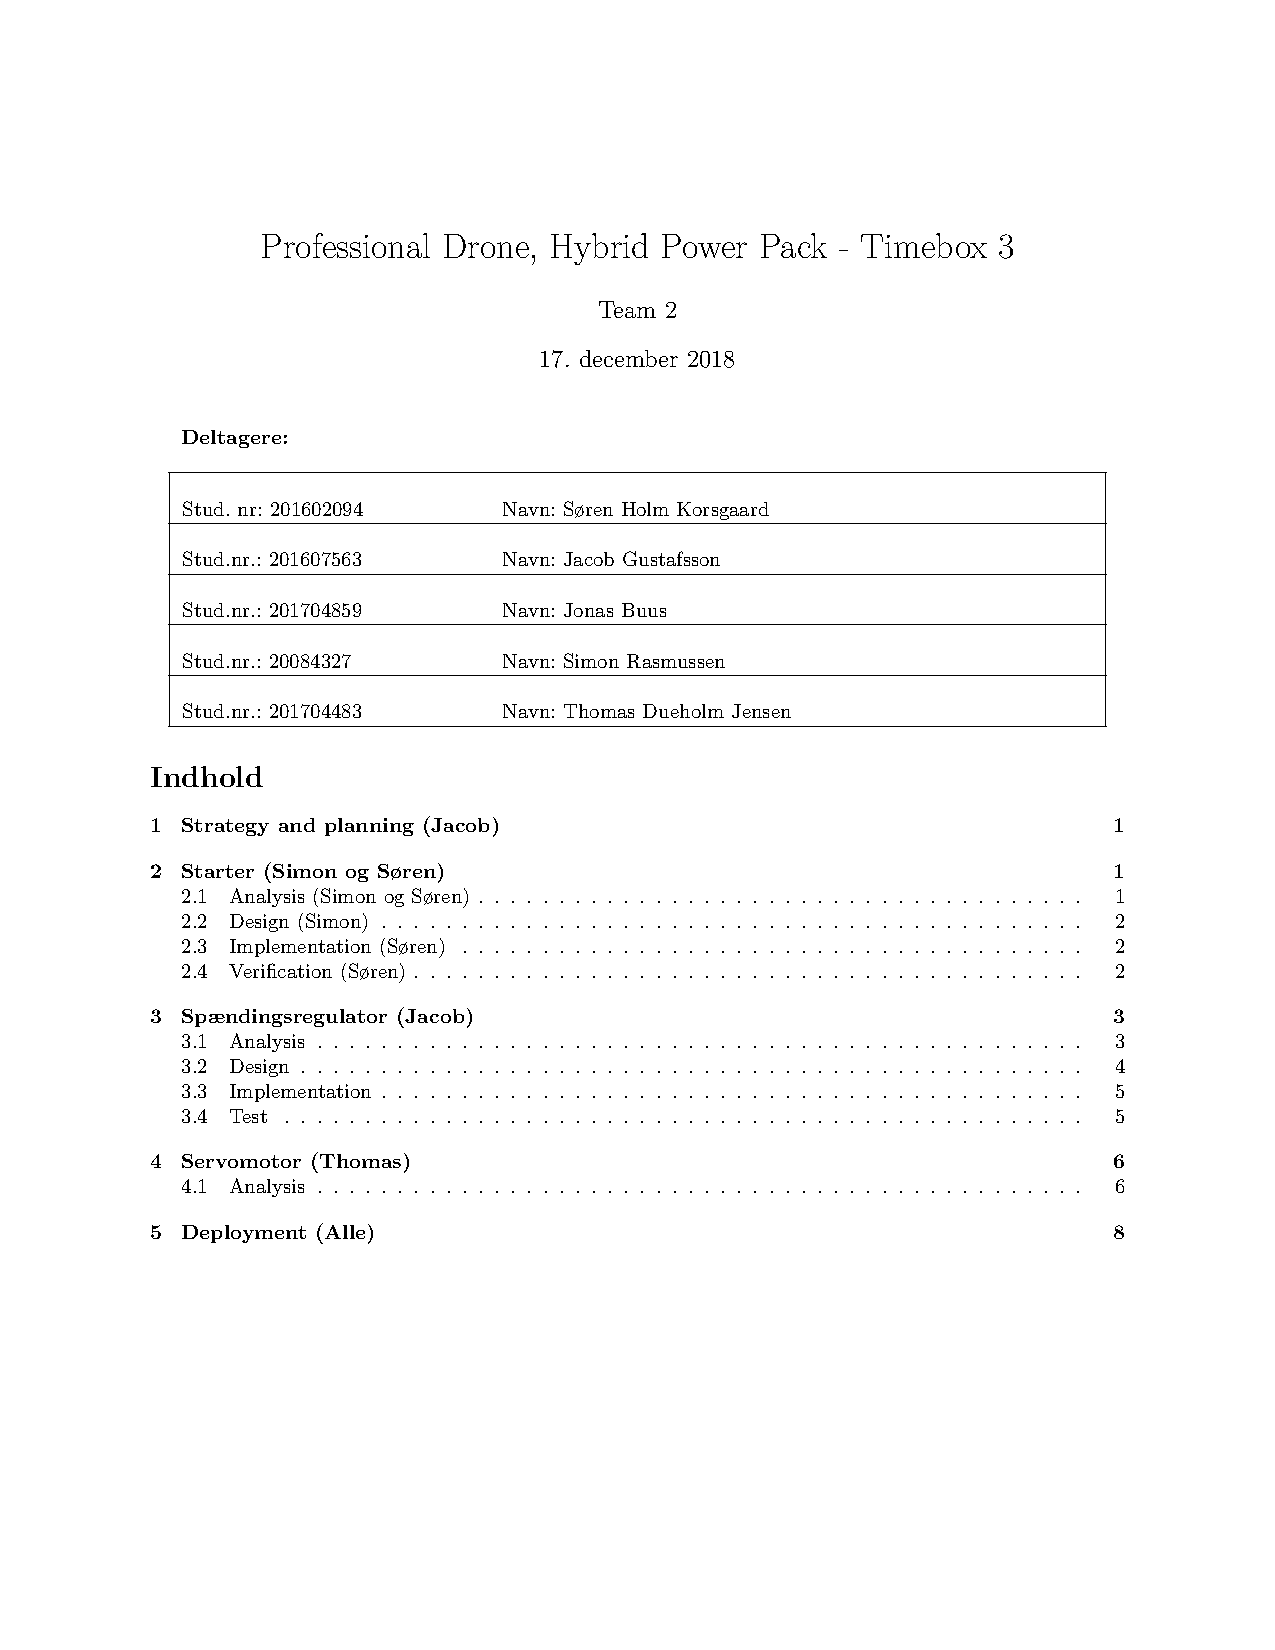
\includepdf[pages={-}]{timebox3-171218}
% \clearpage

% \addcontentsline{toc}{section}{Timebox 4}
% \label{sec:timebox-4-1}
% 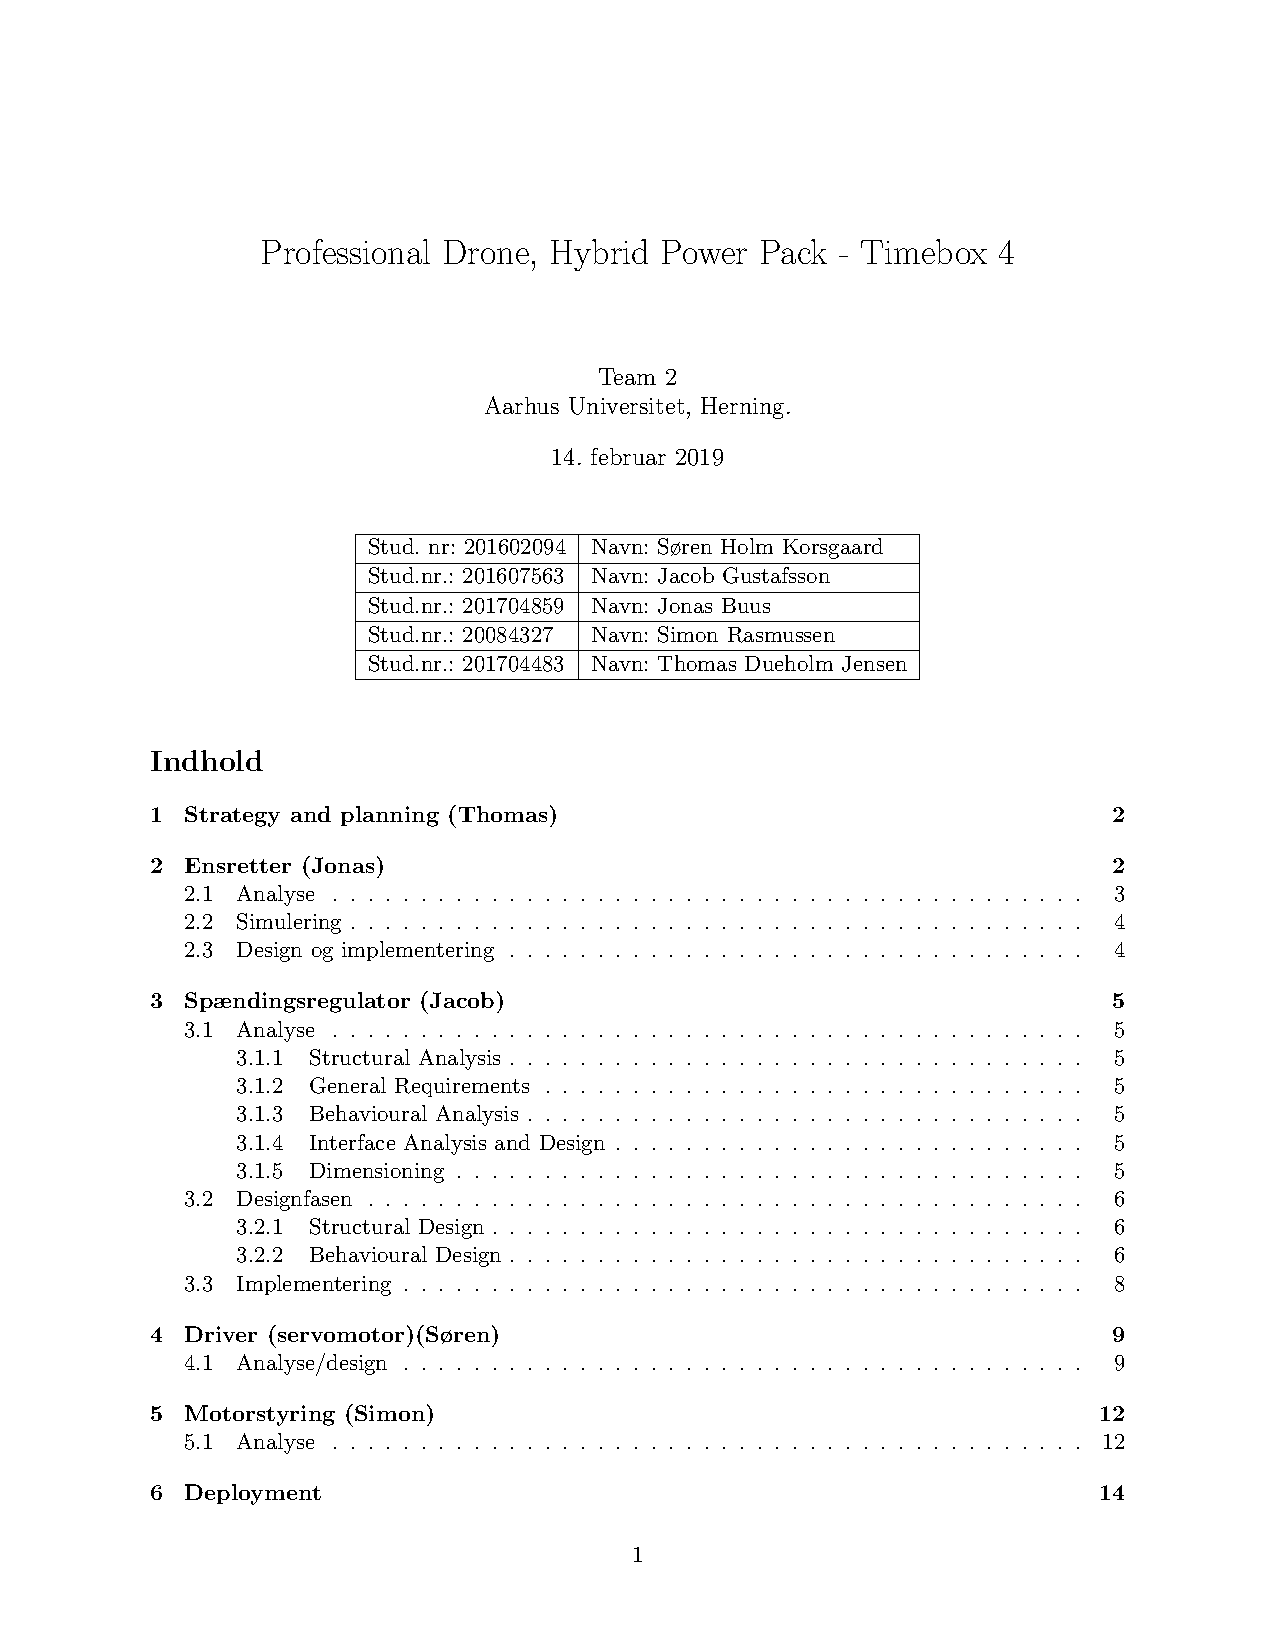
\includepdf[pages={-}]{timebox4-140219}
% \clearpage

% \addcontentsline{toc}{section}{Timebox 5}
% \label{sec:timebox-5}
% \includepdf[pages={-}]{timebox5-280219}
% \clearpage

% \addcontentsline{toc}{section}{Timebox 6}
% \label{sec:timebox-6}
% \includepdf[pages={-}]{timebox6}
% \clearpage

% \addcontentsline{toc}{section}{Timebox 7}
% \label{sec:timebox-7}
% \includepdf[pages={-}]{timebox7}
% \clearpage

% \addcontentsline{toc}{section}{Timebox 8}
% \label{sec:timebox-8}
% \includepdf[pages={-}]{timebox8}
% \clearpage

% \addcontentsline{toc}{section}{Timebox 9}
% \label{sec:timebox-9}
% \includepdf[pages={-}]{timebox9}
% \clearpage

\chapter{Procesevaluering}
\label{cha:procesevaluering}

\section{Indledning}
\label{sec:indledning}

I dette afsnit vil vi beskrive vores proces gennem projektet. Vi kommer ind på arbejdsfordeling, roller, planlægning og hvordan det har været at skabe en struktur for projektet.

\section{Gruppedannelse, samarbejdsaftale og udviklingsforløb}
\label{sec:gruppe-dannelse:-}

Sammensætning af vores gruppe, er ud fra vores insights personlighedsprofiler, vi fik lavet i starten af uddannelsen. Vi er en blanding af forskellige profiler, hvilket skaber en dynamik og til tider en anderledes tilgang til tingene. Det giver mulighed for at belyse hver opgave med et bredt perspektiv.  

% \section{Samarbejdsaftale}
% \label{sec:samarbejdsaftale:-}

Vi lavede i starten en psykologisk kontrakt, hvori vi har beskrevet vores forventninger til hinanden og til gruppen. Der er opsat kriterier, man skal opfylde for at kunne blive i gruppen. % I tilfælde af hvis der var en i gruppen som ikke levede op til disse kriterier. Og hvordan dette skulle tackles, disse kriterier er vi alle enige i, og har underskrevet dette.
Kontrakten kan ses i bilag ()

% \section{Udviklingsforløb}
% \label{sec:udviklingsforlob}

Vi har anvendt EUDP værktøjet til vores udvikling. Se fodnote http://eudp.dk/index.php/Main_Page

\section{Projektledelsen}
\label{sec:projektledelsen}

I starten af projektet valgte vi at give hinanden en rolle i vores projekt, så man havde et ansvarsområde. Rolleinddelingen kan ses i tabel \ref{tab:rolle}.
\begin{table}[h]
  \centering
% BEGIN RECEIVE ORGTBL rolle
\begin{tabular}{ll}
\textbf{Navn} & \textbf{Rolle} \\
\hline
Søren & Projektleder \\
Simon & Ordstyrer til møder samt sammensætning af rapporter \\
Thomas & Holder styr på deadlines og indkaldelse til vejledningsmøder og kundemøder \\
Jacob & Referent til ugentlige møder \\
\end{tabular}
% END RECEIVE ORGTBL rolle    
  \caption{Rollefordeling}
  \label{tab:rolle}
\end{table}
\begin{comment}
#+ORGTBL: SEND rolle orgtbl-to-latex :splice nil :skip 0
| Navn:  | Rolle:                                                                     |
|--------+----------------------------------------------------------------------------|
| Søren  | Projektleder                                                               |
| Simon  | Ordstyrer til møder samt sammensætning af rapporter                        |
| Thomas | Holder styr på deadlines og indkaldelse til vejledningsmøder og kundemøder |
| Jacob  | Referent til ugentlige møder                                               |
\end{comment}

\section{Arbejdsfordeling og planlægning}
\label{sec:arbejdsfordeling:-}

Arbejdsopgaver blev uddelt udfra hvad man havde interesse for og lyst til. Da Søren er uddannet mekaniker, var det naturligt at han skulle stå for mekanikken. 

% \section{Planlægning}
% \label{sec:planlagning:-}


Som det ses i figur \ref{fig:p1} og i launch fase, se bilag, har vi lavet et Gantt-skema. Så vi fik tildelt hver en opgave, som vi skulle arbejde med og gøre færdigt og hvis der opstod problemer eller man skulle have hjælp, kunne man bare spørge tilrådes ved hinanden, så opgaven bedre kunne løses, hvilket også er beskrevet i vores psykologiske kontrakt.

\begin{figure}[h]
  \centering
  \includegraphics[width=0.6\textwidth]{./figurer/p1.png}
  \caption{Development plan}
  \label{fig:p1}
\end{figure}

%Gantt-skemaet i figur \ref{fig:p1} viser planlægningen af vores projekt. %Men forbehold for at der er ting som kan tage længere tid end forventet, derfor er dette kun et udgangspunkt og bliver muligvis rettet under udviklingen i projektet.

\section{Projektadministration}
\label{sec:proj-}

Deling af materiale foregik på GitHub.% Og ellers Facebook gruppe og telefon kontakt.
Da vores gruppe består af onliner og campusstuderende havde vi et fast video-møde hver mandag kl. 20. hvor vi har haft en opsamling og diskuteret udfordringer.

\section{Konflikthåndtering og udfordringer}
\label{sec:konfl-}

I det første halve år, af vores projekt, gik det hele efter planen. Men da vi kom i gang igen i det nye år, meldte Jonas ud, at han er i samtale med studievejledningen om at få forlænget sit studie, hvilket medførte, at han ikke forsatte. 

Derfor gik Søren fra timebox 7, med i arbejdte med ensretteren. Dette betød, at vi kun havde en mand på motorstyringen i stedet for to. Denne rokering betød at vores tidsplan blev rykket. Alle realiseringer tog meget længere tid end beregnet. Ensretteren virkede ikke som forventet og vi brugte meget tid på at prøve at finde en løsning på dette. De  gange vi brugte på at lave en test på vores motor, brugte vi ofte bare en time på at opstille det og ofte havde onlinere også det problem, at de ikke havde sufficient hardware, for at kunne teste og verificere deres opgaver.
I timebox 6, var vi nødt til at stoppe arbejdet på ensretteren, fordi vi var nødt til at teste spændingerne fra BLDC-motor, for at kunne forsætte.

\chapter{Konklusion og diskussion}
\label{cha:konkl-og-disk}

% \addcontentsline{toc}{chapter}{\protect\numberline{\thesection}Diskussion}
\section{Diskussion}
\label{sec:diskussion}

% \addcontentsline{toc}{chapter}{\protect\numberline{\thesection}Konklusion}

\section{Konklusion}
\label{sec:konklusion}


\end{document}